\documentclass[12pt]{article}

% =======================================================================
% Variables
% =======================================================================
% \title{Hàbits de lectura en un centre educatiu de l'Hospitalet de Llobregat. \\[3.5ex]
%     \large Anàlisi dels hàbits de lectura per oci de l'alumnat des de 3r d'ESO fins a 2n de Batxillerat i dels factors relacionats en un centre educatiu de l'Hospitalet de Llobregat.}
% \author{Alejandro Campos Almazán}
% \date{Maig, 2026}

\newcommand{\HeaderTitle}{Universitat Oberta de Catalunya -- Treball Final de Màster}
\newcommand{\ReferencesFile}{references}
\newcommand{\Language}{catalan}

\newif\ifstartwithtitle
\startwithtitletrue % Uncomment to start with just title

\newif\ifshowheader
\showheadertrue % Uncomment to have header

\newif\ifshowfooter
% \showfootertrue % Uncomment to have footer

% =======================================================================
% / Variables
% =======================================================================

% =======================================================================
% Main Config
% =======================================================================
% --- How text input is interpreted ---
\usepackage[utf8]{inputenc}
\usepackage[T1]{fontenc}

% --- Language ---
\usepackage[\Language]{babel} 

% --- Automatic language quotation ---
\usepackage{csquotes}

% --- Squares ---
\usepackage{amsfonts}

% --- Math ---
\usepackage{amsmath}

% --- Pictures ---
\usepackage{graphicx}
\usepackage{float}
% Fix caption spacing for figures and tables
\usepackage[justification=centering]{caption}   % centrado de los captions
\captionsetup{skip=0.1pt}

% --- Tables alignment ---
\usepackage{array}

% --- Layout and formatting for title and sections ---
\usepackage{titling}
\usepackage{titlesec}
\usepackage[a4paper]{geometry}
\setlength{\parindent}{0ex}
\setlength{\parskip}{6pt}
\geometry{top=2.5cm, bottom=2.5cm,left=3cm, right=3cm}

% --- Add one more depth degree with paragraph ---
\setcounter{secnumdepth}{5} % Enable numbering for paragraph and subparagraph
\setcounter{tocdepth}{5} % Enable paragraph and subparagraph in the table of contents
\titleformat{\paragraph}
{\normalfont\normalsize\bfseries}{\theparagraph}{1em}{}
\titlespacing*{\paragraph}
{0pt}{3.25ex plus 1ex minus .2ex}{1.5ex plus .2ex}

% =======================================================================
% / Main Config
% =======================================================================

% =======================================================================
% Bibliography
% =======================================================================
% --- APA7 Bibliography ---
\usepackage[style=apa, backend=biber]{biblatex}
%\DeclareLanguageMapping{catalan}{catalan-apa}
\addbibresource{\ReferencesFile}

% --- French layout in Bibliography---
\setlength{\bibhang}{1.27cm}     % sangría francesa (~0.5 pulgadas)
\setlength{\bibitemsep}{0.8\baselineskip}  % separación entre entradas
\setlength{\bibnamesep}{0.8\baselineskip}  % separación adicional entre autores distintos (opcional)

% --- Define nested cites ---
% Freud \nestedtextcite{2025}{perinat}
\newcommand{\nestedtextcite}[2]{%
  (#1, citat a \citeauthor{#2}, \citeyear{#2})%
}

% \nestedparencite{Freud}{2025}{perinat}
\newcommand{\nestedparencite}[3]{%
  (#1, #2, citat a \citeauthor{#3}, \citeyear{#3})%
}

% \nesteddoubleparencite{Freud}{1920}{Erikson}{1960}{perinat}
\newcommand{\nesteddoubleparencite}[5]{%
  (#1, #2; #3, #4, citats a \citeauthor{#5}, \citeyear{#5})%
}

% \nestedparenpagcite{Freud}{2025}{perinat}{p. 33}
\newcommand{\nestedparencitepag}[4]{%
  (#1, #2, citat a \citeauthor{#3}, \citeyear{#3}, #4)%
}

% =======================================================================
% / Bibliography
% =======================================================================

% =======================================================================
% Header | Footer
% =======================================================================
\usepackage{fancyhdr}
\pagestyle{fancy}

% --- Footer ---
\ifshowfooter
  \fancyhf{} % remove previous config
  \fancyfoot[L]{\textit{\HeaderTitle}} % left footer
  \fancyfoot[R]{\thepage} % right footer set to number

  % --- Footer instead of header ---
  \renewcommand{\footrulewidth}{0.4pt}
  \renewcommand{\headrulewidth}{0pt}

  % --- By default first page has the footer ---
  \fancypagestyle{plain}{
    \fancyhf{}
    \fancyfoot[L]{\textit{\HeaderTitle}}
    \fancyfoot[R]{\thepage}
    \renewcommand{\footrulewidth}{0.4pt}
  }
\fi

% --- Header ---
\ifshowheader
  \fancyhf{} % remove previous config
  \fancyhead[L]{\textit{\HeaderTitle}}
  \fancyhead[R]{\thepage}
  \renewcommand{\headrulewidth}{0.4pt}
  \setlength{\headheight}{14pt}

  % --- By default first page has the header ---
  \fancypagestyle{plain}{
    \fancyhf{}
    \fancyhead[L]{\textit{\HeaderTitle}}
    \fancyhead[R]{\thepage}
    \renewcommand{\headrulewidth}{0.4pt}
  }
\fi

% =======================================================================
% / Header | Footer
% =======================================================================

% =======================================================================
% Block templates
% =======================================================================
\usepackage[dvipsnames]{xcolor}
\definecolor{LightGreen}{rgb}{0.56,0.93,0.56} % RGB aproximado
\usepackage{tcolorbox}
\tcbuselibrary{skins,breakable}

\newenvironment{note_blue}[1]{%
    \tcolorbox[beamer,%
    noparskip,breakable,
    colframe=Blue,%
    colbacklower=LimeGreen!75!LightGreen,%
    title=#1]}%
    {\endtcolorbox}

\newenvironment{note_violet}[1]{%
    \tcolorbox[beamer,%
    noparskip,breakable,
    colframe=Violet,%
    colbacklower=Black,%
    title=#1]}%
    {\endtcolorbox}

\newenvironment{note_green}[1]{%
    \tcolorbox[beamer,%
    noparskip,breakable,
    colframe=Green,%
    colbacklower=LimeGreen!75!LightGreen,%
    title=#1]}%
    {\endtcolorbox}

\newenvironment{warning}[1]{%
    \tcolorbox[beamer,%
    noparskip,breakable,
    ,colframe=Red,%
    colbacklower=LimeGreen!75!LightGreen,%
    title=#1]}%
    {\endtcolorbox}
% =======================================================================
% / Block templates
% =======================================================================

% =======================================================================
% No number sections
% =======================================================================
\newcommand{\sectiononumber}[1]{%
  \section*{#1}
  \phantomsection
  \addcontentsline{toc}{section}{#1}
}

\newcommand{\subsectiononumber}[1]{%
  \subsection*{#1}
  \phantomsection
  \addcontentsline{toc}{subsection}{#1}
}

\newcommand{\subsubsectiononumber}[1]{%
  \subsubsection*{#1}
  \phantomsection
  \addcontentsline{toc}{subsubsection}{#1}
}
% =======================================================================
% / No number sections
% =======================================================================

% =======================================================================
% Secondary Config
% =======================================================================
% --- Mainly unused ---
% \usepackage{graphicx}
% \usepackage{amsmath}
% \PassOptionsToPackage{svgnames}{xcolor}
% \usepackage{lipsum}
% \usepackage{verbatim}
% \tcbuselibrary{skins,breakable}
% \usetikzlibrary{shadings,shadows}
% \usepackage{listings}
% \usepackage{amssymb}
% \usepackage{multirow} % for Tables
% \usepackage{fancyvrb} % for "\Verb" macro
% \VerbatimFootnotes % enable use of \Verb in footnotes
% \usepackage{listings}
% \lstset{basicstyle=\ttfamily,
%   showstringspaces=false,
%   commentstyle=\color{green},
%   keywordstyle=\color{blue}
% }

% --- Black Hyperlinks ---
\usepackage[
    colorlinks=true,
    linkcolor=black,
    citecolor=black,
    urlcolor=black
]{hyperref}

% =======================================================================
% / Secondary Config
% =======================================================================

% =======================================================================
% Examples
% =======================================================================
% --- Pictures ---
% \begin{figure}[h]
%     \centering
%     \includegraphics[width=0.8\textwidth]{pictures/organigrama-tecla-sala.png}
%     \caption{Organigrama Tecla Sala.}
%     \label{fig:organigrama-tecla-sala}
% \end{figure}

% --- Tables ---
% \begin{tabular}{|p{2.7cm}|p{6.5cm}|p{5.7cm}|} 
% \hline
% \textbf{Component} & \textbf{Dibuix} & \textbf{Funció} \\[6pt] 
% \hline
% \raggedright\arraybackslash Placa Base Smart Cutebot & blabla & blabla \\
% \hline
% \raggedright\arraybackslash Micro:bit & 
% \vspace{0.5px}
% \centering
% \includegraphics[width=6cm]{pictures//micro-bit.jpeg}
% & Microcontrolador dissenyat per a l'aprenentatge que es pot integrar amb diferents perifèrics. \\
% \hline
% \end{tabular}

% --- Blocks ---
% \begin{warning}{Warning!}
% Comproba que el teu kit d'Smart Cutebot conté tots els elements de la taula anterior. 
% \end{warning}
% \begin{note_violet}{Note}
% Comproba que el teu kit d'Smart Cutebot conté tots els elements de la taula anterior. 
% \end{note:violet}
% =======================================================================
% / Examples
% =======================================================================

% =======================================================================
% Document
% =======================================================================
\begin{document}

\begin{titlepage}
    \centering
    
    % Nombre del centro o universidad
    {\scshape\Large Universitat Oberta de Catalunya \par}
    \vspace{2cm}
    
    % Título
    {\Huge
    Hàbits de lectura en un centre educatiu de l'Hospitalet de Llobregat\par
    % \vspace{0.5cm}
    }

    \vspace{1cm}
    
    % Subtítulo
    {\Large
    Anàlisi dels hàbits de lectura de l'alumnat adolescent i dels factors relacionats en un centre educatiu de l'Hospitalet de Llobregat.
    \par}

    \vspace{3cm}
    
    % Autor
    {\Large
    Assignatura: Treball Final de Màster\par}
    
    \vspace{4cm}
    
    % Autor
    {\Large
    Alejandro Campos Almazán\par}
    
    \vspace{0.5cm}
    
    % Tutor/a
    {\large Tutor: David Hugas Germa}

    \vspace{0.5cm}

    % Rectora/a
    {\large Rectora: Àngels Fitó Bertran}
    
    \vspace{2cm}
    
    % Información adicional
    {\large
    Curs 2025--2026}
    
    \vspace{0.5cm}

    % Fecha
    {\large
    2 de Juny de 2026}
\end{titlepage}

\thispagestyle{empty}   % suppress page number 
\setcounter{page}{0}  % start content on the next page
\newpage
% =======================================================================

\section{Abstract}
% =======================================================================

//WIP: Pendent per l'entrega final.

\textbf{Keywords:} hàbits de lectura, adolescència, context educatiu, dispositius digitals, entorn familiar pro-lector, lectura activitat social.

\newpage
\tableofcontents
\listoffigures
\listoftables
\newpage

% \ifstartwithtitle
%   \thispagestyle{empty}   % suppress page number 
%   \setcounter{page}{0}  % start content on the next page
%   \newpage
%   \tableofcontents
%   \newpage
% \fi

\newpage
\section{Introducció}
% =======================================================================
% La introducció ha de presentar l’orientació i les motivacions generals que han conduït al desenvolupament del treball, així com argumentar de manera coherent la pertinència i l’interès de la recerca que es proposa. També ha de contenir l’estructura del treball que es presenta, posant en relleu els apartats més importants que s’hi tractaran. Abans d’escriure la introducció del TFM us recomanem llegir l’apartat «5.1.2 Introducció» del material L’informe d’investigació que us donarà una pauta sobre com fer-la.
\label{intro}

\subsection{Context}

Llegir és una activitat que ens defineix com a espècie, que ens ha permès durant mil·lennis transmetre el coneixement entre persones, generacions i cultures \parencite{shutaleva}. La lectura és una activitat que implica tots els tipus de raonament: lògic, crític, creatiu, analític, imaginatiu, empàtic i reflexiu \parencite{chiweta_sm}; i és utilitzada globalment com a eina per a l'aprenentatge, la creativitat, l'entreteniment, l'expressió d'emocions, la reflexió, la transmissió d'històries i experiències, la preparació d'estratègies, entre d'altres.

Entre el mite i la realitat, es diu que Alexandre Magne dormia amb una còpia de la Ilíada sota el coixí en les seves campanyes militars \parencite{plutarc}, que Juli Cèsar preparava estratègies militars a través de la lectura i l'escriptura mentre la resta de generals descansaven, que Cleopatra va créixer jugant entre llibres a la gran biblioteca d'Alexandria \parencite{posteguillo_maldita}, que Napoleó viatjava a les seves campanyes militars amb una biblioteca portàtil amb centenars de llibres i que Winston Churchill es va negar a reduir el pressupost de cultura dels Estats Units per destinar-ho al finançament de la Segona Guerra Mundial \parencite{posteguillo_tertulia}, entre molts d'altres.

\subsection{Beneficis de la lectura}

Segons estudis recents, la lectura és una activitat que comporta nombrosos beneficis cognitius, emocionals, socials i educatius. Ja des de ben petits, tal com expliquen \textcite{goikoetxea_lectura}, la lectura compartida afavoreix el desenvolupament del llenguatge, la comprensió i el coneixement. La lectura és una activitat que estimula el creixement cerebral, la profunditat emocional i les habilitats comunicatives; alhora que afavoreix la retenció de coneixement, la reflexió, el pensament crític i el coneixement profund \parencite{ataniyazova}. 

Llegir per plaer durant la infància s'associa amb una millor memòria, desenvolupament cognitiu, desenvolupament del llenguatge, hàbits de son, habilitats comunicatives i salut mental \parencite{sun_childhood}. Altres estudis com \textcite{billington_reading} conclouen que la pràctica de la lectura per plaer està vinculada a una major autoestima, autoacceptació, creativitat, habilitats socials i empatia. La lectura freqüent es relaciona amb un menor risc de deteriorament de les funcions cognitives en persones grans i millors resultats en tots els nivells educatius \parencite{chang_reading}. \textcite{banas_biblio} conclouen que la participació en clubs de lectura es correlaciona amb millors habilitats psicosocials i un major benestar.

D'altra banda, la lectura és considerada una activitat en la que es practica l’atenció plena o \emph{mindfulness}, ja que requereix focalitzar l’atenció de manera sostinguda, reduir les distraccions i estar activament en el moment present per comprendre el text i endinsar-se en la narració \parencite{gorsy}. En aquest sentit, la pràctica de l'atenció plena s’ha relacionat àmpliament amb una millora del benestar, tant físic com psicològic, la salut i la regulació de les emocions \parencite{baena}.

Finalment, el marc normatiu català actual sustenta que la lectura, com a base d’altres aprenentatges, esdevé un factor fonamental per a l’adquisició i el desenvolupament de les competències bàsiques. També subratlla que saber llegir ens permet créixer com a persones, desenvolupar el coneixement i interactuar en la nostra societat. Per aquest motiu, fomentar i treballar la lectura ha de ser una prioritat en els centres educatius i en la tasca de tot docent, independentment de l'àrea o matèria que s'imparteixi \parencite{generalitatPLEC}.

\subsection{La lectura com activitat sociocultural}

Les pràctiques culturals constitueixen un pilar fonamental del comportament humà, comprenent un ventall ampli d'activitats com costums socials, rituals, tradicions, normes, valors, formes d'expressar-se, etc. \parencite{shutaleva}. Aquestes pràctiques proporcionen un marc per a la interacció entre individus i defineixen la identitat d'una societat, donant lloc a patrons culturals que no són fixes ni immutables, sinó que evolucionen constantment en resposta a canvis socials, polítics, econòmics i tecnològics del context històric \nesteddoubleparencite{Kirillova et al.}{2022}{Hofstede et al.}{2009}{shutaleva}.

La lectura és una pràctica cultural que depèn del context històric concret, però que alhora contribueix a modelar-lo i transformar-lo. Sovint entenem el llenguatge, i per tant la lectura, com a mera eina per transmetre la informació que ja hi és a la nostra ment (metàfora de la conducció; Michel Reddy, 1979, citat a Gil Juárez i Vitores González, 2009). Res més allunyat de la realitat, ja que el llenguatge, i en conseqüència la lectura, construeixen i modelen la interpretació individual i col·lectiva de la realitat \parencite{gil_comu}. <<Els límits del nostre llenguatge són els límits del nostre món>> \nestedparencite{Wittgenstein}{1922}{lanza_wittgenstein}. D'aquesta manera, la lectura és causa i alhora conseqüència del context sociocultural d'una època. 

En aquest estudi analitzarem la lectura des d'un punt de vista transversal, com una activitat que s'integra en el context sociocultural d'un centre de l'Hospitalet de Llobregat, però que alhora contribueix a modelar-lo i transformar-lo. D'aquesta manera, no s'entén la lectura com una activitat aïllada, sinó com una pràctica cultural influenciada per múltiples factors, però que alhora té un paper actiu en la conformació d'aquest context.

\textcite{shutaleva} assenyalen que factors com el nivell d'estudis dels pares, la disponibilitat d'una biblioteca a casa, la implicació paternal en la lectura dels joves i el fet de tenir amb qui compartir les experiències lectores són factors que es correlacionen positivament amb la dedicació a la lectura.

\subsection{Lectura, adolescència i actualitat}

La irrupció en les últimes dècades de les tecnologies digitals està transformant la forma en com les persones accedim a la informació, produïm dades, ens comuniquem, ens relacionem, ens entretenim, etc.

Internet, els buscadors, les plataformes multimèdia, les xarxes socials, les plataformes de vídeos curts, les eines d'IA, entre d'altres ocupen moltes hores en el dia a dia dels joves i adolescents \parencite{shutaleva} ---i també en adults---. Però són aquestes eines competidores directes de l'activitat lectora? No hi ha un consens clar al respecte en la literatura científica existent, ja que alguns estudis conclouen que l'ús de xarxes socials es correlaciona negativament amb el temps dedicat a la lectura de forma significativa \parencite{owusu_sm}, mentre que altres estudis no troben prou significació per sostenir aquesta afirmació \parencite{shutaleva}. 

Parlant amb diferents adolescents del meu entorn i alumnes del centre de pràctiques he tingut la sensació que, una gran majoria, no llegeix llibres o còmics per oci mai o quasi mai i que no tenen hàbits de lectura, ni a casa ni a l'escola. Quan els hi he preguntat per què no llegeixen, molts d'ells m'han dit que no els agrada, que és avorrit, que prefereixen altres activitats, que no els aporta res o que no tenen temps. D'altra banda, una gran majoria d'ells i elles dediquen una quantitat considerable d'hores al dia a l'ús d'eines digitals, xarxes socials i plataformes de contingut audiovisual.

També he observat que molts d'ells presenten dificultats a l'hora de comprendre diferents textos que se'ls proposa, com enunciats d'exercicis, textos informatius, guies de treball, etc.; i que els costa extreure la informació rellevant d'un text o mantenir l'atenció i el fil de la lectura quan aquesta és llarga. 

Tot i que principalment he observat i co-impartit assignatures de ciències, he percebut que molts dels errors que acostumen a cometre els alumnes no són per no conèixer els conceptes de l'assignatura, sinó per errors de comprensió dels enunciats, per no llegir amb prou atenció, per no saber extreure la informació rellevant o per no saber interpretar dades o gràfics.

Tanmateix, em fa l'efecte que en l'àmbit educatiu, cada vegada es treballen menys les competències relacionades amb la lectura i la comprensió escrita en general, i que la tendència sembla orientar-se cap a la fragmentació i simplificació de la informació per convertir-la en contingut de comprensió immediata i accessible per a tothom, especialment a través de formats audiovisuals, interactius i ràpids, cognitivament més assequibles.

\newpage
\section{Definició del problema, preguntes i objectius de la recerca}
% =======================================================================
% Aquest apartat del TFM ha de contenir el problema que s’ha detectat i que es vol investigar, la pregunta que serveix de base per al disseny de la investigació i els objectius (general i específics). L’objectiu general de la recerca es desplegarà en un conjunt d’objectius específics prou concrets i operatius (avaluables).
Partint del context descrit en l'apartat \nameref{intro}, he volgut enfocar la meva investigació en la composició d'una fotografia completa dels hàbits de lectura de l'alumnat adolescent en el meu centre de pràctiques. En concret, es pretén descriure variables com el temps dedicat a la lectura per oci, les preferències temàtiques, els formats més utilitzats, la quantitat de lectures realitzades anualment i la percepció de l’alumnat envers la lectura, així com el grau de seguiment de les lectures obligatòries, l’ús de recursos com resums o eines d’IA generativa, la freqüència de visites a la bilblioteca, etc.

D'altra banda, també es pretén analitzar factors potencialment associats a aquests hàbits, com l’ús de tecnologies digitals i xarxes socials, el consum de continguts audiovisuals, l’entorn familiar i social, la percepció i discurs adolescent sobre la lectura, la participació en activitats lectores compartides, el gust per les lectures obligatòries i la relació amb altres pràctiques d’oci.

D'aquesta manera, la pregunta de recerca que guia aquest estudi és: quins són els hàbits de lectura de l’alumnat adolescent del centre educatiu estudiat i quins factors es troben associats al seu desenvolupament?

En coherència amb aquesta pregunta, l’objectiu general de la recerca és descriure de forma detallada i exhaustiva els hàbits de lectura de l’alumnat adolescent en el centre d'estudi, així com de les possibles variables que hi poden estar relacionades.

Aquest objectiu general es concreta en els següents objectius específics:

\begin{itemize}
    \item Descriure la freqüència, formats i preferències temàtiques de lectura per oci de l’alumnat.
    \item Caracteritzar les sessions de lectura de l'alumnat i explorar les visites a la biblioteca per a agafar llibres o còmics en préstec.
    \item Analitzar el grau de compromís i gust per les lectures obligatòries del centre i la seva relació amb el desenvolupament de l’hàbit lector.
    \item Analitzar l’ús de tecnologies digitals i xarxes socials en relació amb els hàbits lectors.
    \item Analitzar altres activitats d'oci realitzades per l'alumnat i la seva relació amb els hàbits de lectura per oci.
    \item Explorar la relació entre els hàbits de lectura de l’alumnat i el seu entorn social i familiar.
\end{itemize}

A partir d’aquesta diagnosi, es pretén disposar de bases sòlides per a plantejar estratègies educatives que fomentin la motivació, l’interès i el desenvolupament de la lectura en el context acadèmic.

\newpage
\section{Estat de la qüestió, marc teòric i normatiu}
% =======================================================================
% En aquest apartat s’ha d’exposar el marc teòric en el qual es fonamenta la recerca: les teories i conceptes que es troben directament vinculats amb l’estudi i l’estat de la qüestió, és a dir, la presentació breu d’estudis similars, amb els seus resultats més destacats i la connexió amb la recerca que es proposa al TFM. El marc normatiu existent que sustenta la recerca fa referència a les lleis o polítiques públiques educatives (espanyoles i catalanes) i a altres documents normatius del centre, relacionats amb la temàtica de la recerca.
Analitzant la literatura existent, diversos estudis han analitzat els hàbits de lectura dels joves i com aquests es veuen influenciats per factors tecnològics, socials i familiars. Tanmateix, es poden identificar tendències comunes i resultats divergents.

En primer lloc, segons l'Informe de resultados de Hábitos de lectura y compra de libros en España \nestedtextcite{2018}{sanches}, el 44.7\% dels joves entre 15 i 18 anys és lector freqüent, mentre que el 22.7\% és lector ocasional i el 32.6\% es declara no lector. Per aquest motiu, \textcite{sanches} suggereixen que la lectura s'està convertint en una activitat obligada per qüestions pràctiques, oblidant la forta relació entre el rendiment acadèmic i el gaudir per la lectura.

D'altra banda, l’estudi de \textcite{shutaleva} conclou que la lectura continua sent una activitat present en l’oci juvenil, tot i la creixent presència de les tecnologies digitals. L’estudi destaca la importància del context familiar, ja que factors com el nivell educatiu dels pares, la disponibilitat de llibres a casa o la implicació parental en la lectura durant la infància es correlacionen positivament amb la dedicació lectora en etapes posteriors. Així mateix, es posa de manifest que les noies tendeixen a compartir més les seves experiències lectores, mentre que no es troben diferències significatives en la quantitat de lectura entre gèneres. Aquest estudi també suggereix que el format de lectura predominant continua sent el llibre físic, tot i l’augment progressiu dels formats digitals i els audiollibres.

En una línia complementària, \textcite{akande_library} analitzen la relació entre l’ús de xarxes socials i els hàbits de lectura en estudiants de secundària a Nigèria. Els resultats mostren una correlació negativa significativa entre el temps dedicat a les xarxes socials i el temps dedicat a la lectura per oci, suggerint una possible competència temporal entre ambdues activitats.

Tanmateix, l’estudi longitudinal de \textcite{johnsson_bookreading} aporta una perspectiva dels hàbits lectors al llarg de 25 anys. Els resultats mostren que, malgrat l’augment significatiu de l’ús de tecnologies digitals, el temps dedicat a la lectura no ha disminuït de manera proporcional, i fins i tot ha augmentat en determinats grups. En aquest sentit, no es troba una correlació clara entre l’ús de tecnologies i la lectura per oci, qüestionant la idea d’una competència directa entre ambdues activitats. L’estudi sí que identifica una lleugera correlació negativa entre el temps dedicat a veure televisió i la lectura.

Una altra conclusió interessant d'aquest estudi és que la lectura s'ha polaritzat lleugerament amb el pas del temps: s'ha incrementat el nombre d'adolescents que no llegeixen mai per oci, mentre que els que ja llegien han augmentat el temps de lectura. Quant al gènere, els resultats de l'estudi mostren que hi ha molts més nois que no llegeixen mai per oci que noies. Finalment, els autors conclouen que els hàbits de lectura estan més condicionats pel context familiar i social que no pas per l’ús de tecnologies digitals.

Des del marc normatiu català, es destaca la gran importància de la lectura en l'adquisició del coneixement, el desenvolupament personal i la interacció social \parencite{generalitatPLEC}. En aquest sentit, es subratlla la necessitat de tenir un PLEC (Pla de Lectura de Centre), per aconseguir una coordinació pedagògica entre els diferents agents educatius que promogui el gust per la lectura i el saber llegir des de totes les àrees del currículum.

\newpage
\section{Metodologia}
% =======================================================================
% El TFM ha de contenir informació clara i coherent sobre la perspectiva metodològica de l’estudi, així com la justificació de l’elecció del mètode que segueix la investigació per aconseguir els objectius plantejats. Aquest apartat també ha d’incloure els següents subapartats:

\subsection{Disseny de recerca i mostra}
% ---------------------------------------------------
El present estudi adopta un disseny d'investigació no experimental, de caràcter descriptiu i transversal de tipus estudi de cas. És a dir, la recollida de dades s'ha realitzat en un únic moment temporal, i per tant, els resultats no poden afirmar relacions de causalitat direccional entre les variables analitzades.

D'altra banda, el disseny de cas no pretén generalitzar els resultats a altres contextos o la població general, sinó que se centra en l'anàlisi exhaustiva i detallada d'un cas concret, en aquest cas, un centre educatiu de l'Hospitalet de Llobregat.

L’enfocament metodològic d'aquesta recerca ha estat mixt de tipus convergent o concurrent, recollint de manera paral·lela dades quantitatives i qualitatives. Posteriorment, els resultats d'ambdues aproximacions s'han comparat, contrastat i integrat mitjançant triangulació per interpretar de forma global els hàbits de lectura de l'alumnat adolescent i els diferents factors associats al seu desenvolupament.

Per tal de mantenir la coherència d'exhaustivitat, la mostra d'anàlisi quantitativa (alumnes als quals se’ls ha subministrat el qüestionari) s'ha conformat mitjançant la tècnica de mostreig no probabilística per conglomerats, seleccionant com a unitats d’anàlisi els grups-classe corresponents als cursos des de 3r d’ESO fins a 2n de Batxillerat del centre en qüestió.

Després de 3 setmanes de reunions, coordinació i acords amb el centre i els diferents docents implicats, tanquem la recollida de dades quantitatives com un èxit: s'ha subministrat el qüestionari a tots els alumnes de totes les classes a excepció d'un grup de 4t d'ESO, que no ha pogut participar per motius organitzatius i de coordinació. En total, s'ha subministrat el qüestionari a 343 alumnes.

No s'ha estès l'estudi a altres cursos (com per exemple, 1r i 2n d'ESO) a causa de les limitacions temporals i de recursos disponibles per a la realització d'aquesta recerca, així com per mantenir la coherència amb els objectius plantejats, que se centren en l'anàlisi dels hàbits de lectura en l'etapa adolescent.

La mostra qualitativa de l’estudi s'ha conformat mitjançant mostreig no probabilístic per conveniència, seleccionant alumnes i professors que, voluntàriament, han acceptat participar en les entrevistes semiestructurades. A partir d'aquest mètode s'han entrevistat 3 docents de les assignatures de Llengua i Literatura Castellana i Catalana i 2 alumnes de 1r i 2n de Batxillerat.


\subsection{Tècniques i instruments de recollida de dades}
% ---------------------------------------------------

Per a la recollida de dades quantitatives s'ha fet ús del mètode d'enquestes, mitjançant l'aplicació d'un qüestionari \emph{ad hoc} dissenyat específicament per aquest estudi, que integra ítems de diferents qüestionaris validats en la literatura existent, adaptats al context i als objectius d'aquesta recerca.

Per a l’anàlisi dels hàbits de lectura i de la influència de l’entorn familiar pro-lector, s’han adaptat ítems dels qüestionaris PIRLS (Progress in International Reading Literacy Study) \parencite{pirls} i HLEQ (Home Literacy Environment Questionnaire) \parencite{hleq}, àmpliament utilitzats per avaluar els hàbits lectors i l’entorn d’alfabetització familiar.

D'altra banda, per analitzar l'ús de les TRIC, s’han adaptat ítems dels qüestionaris EU Kids \parencite{eukids} i ICILS \parencite{icils}, utilitzats a nivell internacional per a l’anàlisi de l’ús de les tecnologies digitals i les xarxes socials.

Finalment, s’inclouen també ítems específics dissenyats per al context concret de l’estudi, com ara analitzar la narrativa i la percepció social sobre la lectura o conèixer les preferències lectores.

% El qüestionari està majoritàriament compost per ítems d'autoclassificació estructurats en escales ordinals graduades, especialment escales tipus Likert, escales de freqüència i escales de resposta categòrica ordenada. Així mateix, s'han inclòs també alguns ítems amb escala de mesura nominal (respostes categòriques dicotòmiques: sí / no, masculí / femení).

La via d’administració del qüestionari ha estat en línia, fent ús de la plataforma Google Forms, per al disseny, la distribució i la recollida de dades; les quals, posteriorment, s'han descarregat en format CSV per tractar-les amb el programari Python 3. Per aquest motiu, el qüestionari s'ha subministrat durant l’horari lectiu amb ordinadors i connexió a internet facilitats pel centre educatiu.

Per a la recollida de dades qualitatives, s'ha optat per utilitzar entrevistes semiestructurades, que han permès obtenir informació detallada i profunda sobre les percepcions, experiències, discursos i narratives dels participants en relació amb els hàbits de lectura i els factors associats, complementant així els resultats obtinguts a partir de la fase quantitativa.

% \subsubsection{Tècniques i instruments de recollida de dades qualitatives}

% Per a la recollida de dades qualitatives, s'ha optat per utilitzar entrevistes semiestructurades amb un grup reduït d'estudiants i professors. Aquest mètode m'ha permès obtenir informació detallada i profunda sobre les percepcions, experiències, discursos i narratives dels participants en relació amb els hàbits de lectura i els factors associats, complementant així els resultats obtinguts a partir de la fase quantitativa.

% Aquestes entrevistes semiestructurades s'han portat a terme de manera presencial al centre educatiu, i han estat enregistrades en format d'àudio per facilitar-ne la posterior transcripció i anàlisi.

\subsection{Aspectes ètics}
% ---------------------------------------------------

En el present estudi s'han garantit els principis ètics fonamentals, com la confidencialitat, l’anonimat i el consentiment informat dels participants. Abans d’iniciar la recollida de dades, s’han explicat de manera clara i detallada els objectius i les finalitats de l’estudi i el seu caràcter voluntari, així com l’ús de les dades i els criteris ètics que se seguirien en el seu tractament.

Quant a les dades, s'han recollit de forma anònima, han estat accessibles únicament per l’investigador principal, s'han tractat de manera confidencial i s'ha garantint que no es pogués identificar cap participant a partir de les respostes proporcionades.

D'igual manera, per a la realització de les entrevistes semiestructurades, s'ha obtingut el consentiment informat dels participants ---en el cas dels adults--- i dels pares o tutors legals ---en el cas dels menors---. Abans de realitzar les entrevistes, s'han explicat els objectius d'aquestes, la voluntarietat de la participació, la possibilitat de retirada en qualsevol moment i la completa confidencialitat de les respostes. També s'ha fet saber l'ús ètic que es faria de les dades recollides, utilitzant-les exclusivament per a les finalitats de la recerca i mantenint l'anonimat dels participants en la presentació dels resultats.

D'altra banda, s'ha procurat que les entrevistes semiestructurades es realitzessin en un entorn còmode i segur per als participants, fomentant un clima de confiança i respecte que permetés una expressió lliure i sincera de les seves opinions i experiències relacionades amb la lectura.

\subsection{Estratègia analítica}
% ---------------------------------------------------
\subsubsection{Estratègia analítica de les dades quantitatives}

S'han exportat les dades recollides al qüestionari en format CSV i, posteriorment, han estat tractades amb el programari Python 3; utilitzant principalment les llibreries \emph{pandas}, \emph{scipy}, \emph{numpy} i \emph{matplotlib}. Si es vol consultar el codi utilitzat per a l'anàlisi de les dades quantitatives, es pot accedir al \href{https://github.com/titocampis/tfm-habits-lectura.git}{\textcolor{blue}{repositori de GitHub de la recerca}}.

En una primera fase, s'ha realitzat una anàlisi descriptiva de les dades, amb l'objectiu de conèixer les característiques generals de la mostra i descriure els hàbits de lectura de l'alumnat a partir del temps mitjà setmanal dedicat a la lectura de llibres o còmics per oci i el nombre de llibres o còmics llegits en els últims 12 mesos per oci. També s'han analitzat descriptivament altres variables relacionades amb la lectura, com les preferències temàtiques i de format, les sessions de lectura, les visites a la biblioteca, etc.

\paragraph{Construcció de la variable nombre de pàgines anuals}

Per tal d’obtenir una aproximació quantitativa del volum total de lectura anual de llibres o còmics per oci, s’ha construït una variable discreta que estima el nombre de pàgines llegides de llibres o còmics en els últims 12 mesos per oci. Aquesta variable s’ha calculat a partir de la combinació de dues variables recollides en el qüestionari: el nombre de llibres o còmics llegits en els últims 12 mesos per oci i el nombre mitjà de pàgines per llibre (ambdues agrupades en categories ordinals d'interval).

Per transformar aquestes variables categòriques en una estimació discreta, s’han assignat valors representatius a cada interval mitjançant el punt mitjà de cada categoria. Posteriorment, s’ha calculat el producte entre el nombre estimat de llibres llegits en l'últim any i la mitjana estimada de pàgines per llibre, obtenint així una aproximació del nombre total de pàgines llegides de llibres o còmics en els últims 12 mesos per oci per cada estudiant.

\[
\text{\emph{Pàgines estimades}} = \text{\emph{Mitjana estimada de llibres}} \cdot \text{\emph{Mitjana estimada de pàgines per llibre}}
\]

Aquesta aproximació permet disposar d’una variable discreta que sintetitza el volum de lectura, facilitant l’anàlisi quantitativa i la comparació entre grups. Tot i això, s'assumeix la limitació derivada de la utilització de valors intermedis estimats a partir de categories ordinals d'interval.

S'ha calculat la correlació de Spearman entre la variable estimada pàgines anuals de llibres o còmics llegits per oci i el temps mitjà setmanal dedicat a aquesta activitat. Els resultats obtinguts ($\rho =$ .823, p < .001) reforcen l'ús d'aquesta variable com a descriptiu dels hàbits de lectura per oci de llibres o còmics de l'alumnat de la mostra.

\paragraph{Construcció de la variable de classificació segons els hàbits de lectura per oci}

Per tal de sintetitzar els hàbits lectors de llibres o còmics per oci de l’alumnat en una única variable interpretable visual i descriptivament, s’ha construït la variable categòrica anomenada \emph{classificació lectora per oci}, que agrupa els participants en tres perfils segons els hàbits de lectura per oci: \emph{no lector / lector molt ocasional}, \emph{lector ocasional} i \emph{lector habitual}. 

La construcció d’aquesta variable de classificació s’ha basat en la combinació de dos indicadors complementaris dels hàbits lectors de llibres o còmics per oci: el temps mitjà setmanal dedicat a aquesta activitat i el volum anual estimat de pàgines llegides. Aquesta aproximació permet integrar tant la freqüència com la intensitat de l’activitat lectora per oci, evitant així dependre exclusivament d’una única mesura parcial del comportament lector.

La categoria de \emph{no lector / lector molt ocasional} s’ha assignat a l’alumnat que no dedica, o dedica poc temps, de mitjana, a la lectura de llibres o còmics per oci ($<$ 30 minuts setmanals), o que presenta un volum anual molt reduït de pàgines estimades llegides de llibres o còmics per oci ($\leq$ 300 pàgines anuals).

\[
\left.
\begin{array}{l}
\text{\emph{Temps de lectura setmanal}} < 30 \text{ minuts} \\\\
\text{\emph{Pàgines estimades llegides anualment}} \leq 300
\end{array}
\right\}
\textit{ No lector / lector molt ocasional}
\]

D'altra banda, la categoria de \emph{lector habitual} s’ha reservat als estudiants que combinen una dedicació considerable de temps mitjà de lectura setmanal de llibres o còmics per oci ($\geq$ 1 hora) amb un volum anual considerable de pàgines estimades llegides de llibres o còmics per oci ($\geq$ 1200).

\[
\left.
\begin{array}{l}
\text{\emph{Temps de lectura setmanal}} \geq 1 \text{ hora} \\\\
\text{\emph{Pàgines estimades llegides anualment}} \geq 1200
\end{array}
\right\}
\textit{ Lector habitual}
\]

Finalment, la categoria de \emph{lector ocasional} agrupa els casos intermedis que no compleixen cap dels criteris extrems anteriors.

Metodològicament, aquesta estratègia permet construir una variable ordinal simplificada capaç de representar diferents nivells d’hàbits lectors per oci, facilitant la interpretació descriptiva dels resultats i la comparació entre grups. Tot i això, cal considerar que es tracta d’una classificació aproximada basada en llindars operatius definits específicament per a aquesta investigació.

Tanmateix, els resultats obtinguts mostren correlacions positives elevades entre la classificació lectora i els principals indicadors utilitzats per a la seva construcció, tant pel que fa al temps mitjà setmanal dedicat a la lectura per oci ($\rho = .864$, $p < .001$), com al nombre de llibres llegits anualment ($\rho = .776$, $p < .001$), com al nombre estimat de pàgines ($\rho = .787$, $p < .001$). Aquestes associacions suggereixen una elevada coherència interna entre la classificació lectora i les diferents dimensions dels hàbits lectors per oci, aportant evidència addicional de consistència i validesa convergent de la variable construïda.

\paragraph{Anàlisi inferencial}

Finalment, s'ha realitzat una anàlisi inferencial amb la finalitat d’explorar la relació entre les diferents variables estudiades i les variables indicadores d'hàbits de lectura per oci. Per a això, s'han utilitzat diferents proves estadístiques segons el tipus de variables analitzades i la seva distribució. En concret, s'han realitzat proves de correlació de Spearman per estudiar la correlació entre variables categòriques ordenades i proves de $\chi^2$ quadrat per analitzar la correlació entre variables categòriques dicotòmiques i ordenades.

Finalment, s'ha elaborat un \emph{heatmap} de correlacions d'Spearman entre les variables indicadores d’hàbit lector per oci i la resta de variables analitzades, amb l'objectiu de tenir una referència visual clara i sintètica d'aquestes associacions.

\subsubsection{Estratègia analítica de les dades qualitatives}

A partir dels enregistraments obtinguts en les entrevistes semiestructurades, s'ha portat a terme un procés de transcripció parcial o selectiva, en què s'han transcrit de manera literal exclusivament aquells fragments de les entrevistes més rellevants. Aquest enfocament ha permès optimitzar el procés de neteja i anàlisi de dades qualitatives sense perdre informació important per als objectius de la recerca.

Finalment, aquestes transcripcions s'han segmentat i categoritzat fent ús d'un sistema de categories que ha permès agrupar els diferents fragments amb l’objectiu d'identificar patrons, recurrències, similituds i divergències en els discursos dels diferents participants.

\subsection{Planificació i implementació del treball de camp}
% ---------------------------------------------------

El treball de camp es va planificar entre els mesos d’abril i maig, estructurant-se en diferents fases relacionades amb la coordinació amb el centre, la validació dels instruments, la recollida de dades i la preparació de l’anàlisi quantitativa i qualitativa.

En una primera fase, es van establir les dates per a l’administració dels qüestionaris als diferents cursos d’ESO i Batxillerat, coordinant amb els responsables de departament i els diferents tutors la compatibilitat amb el calendari escolar i l’accés als ordinadors necessaris per respondre el qüestionari en línia.

Paral·lelament, es van mantenir reunions amb el professorat de llengua i literatura amb l’objectiu de recollir suggeriments de millora del qüestionari i de les entrevistes semiestructurades. Durant aquesta fase també es van acordar les entrevistes amb el professorat participant i es van facilitar els corresponents consentiments informats.

Pel que fa a la recollida de dades qualitatives, es va seleccionar la mostra d’alumnes participants en les entrevistes semiestructurades, es va coordinar amb ells i els seus tutors les hores en les quals es realitzarien aquestes entrevistes i es van gestionar els consentiments informats per part dels pares o tutors legals.

Finalment, entre finals d’abril i principis de maig, es van administrar els qüestionaris als diferents grups participants i es van realitzar les entrevistes semiestructurades a alumnat i professorat, deixant les dades preparades per a la seva posterior anàlisi i triangulació.

\newpage
\section{Resultats del procés d'anàlisi}
% =======================================================================

\subsection{Característiques generals de la mostra}
% ---------------------------------------------------
El qüestionari ha estat subministrat a un total de 343 alumnes de 3r d'ESO fins a 2n de Batxillerat del centre seleccionat, seguint el procediment de mostreig per conglomerats. Del total de la mostra, el 51.9\% ($n =$ 178) són noies, el 45.5\% ($n =$ 156) són nois i el 2.6\% ($n =$ 9) han preferit no respondre. 

\begin{figure}[H]
    \centering
    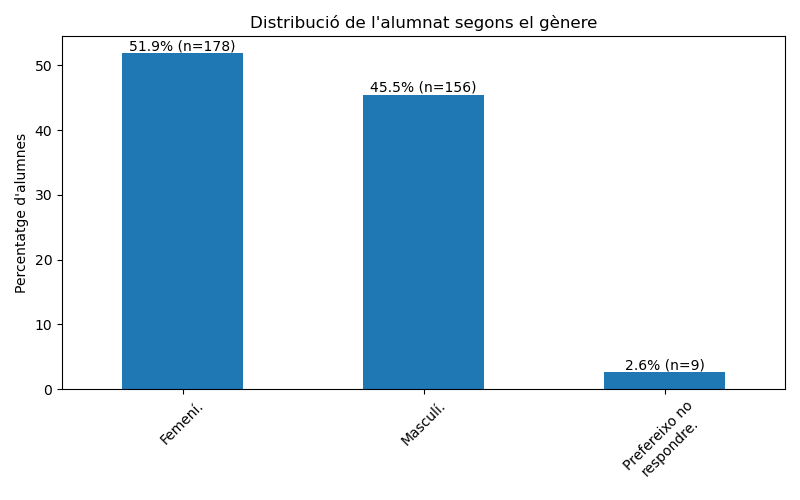
\includegraphics[width=0.85\textwidth]{pictures/1_descriptive_genere.png}
    \caption{Distribució de l'alumnat segons el gènere.}
    \label{fig:descriptive_genere}
\end{figure}

La distribució detallada de la mostra per cursos i modalitat de batxillerat es pot consultar a la \autoref{graf:descript_mostra}

\subsection{Temps de lectura setmanal i llibres o còmics llegits en els últims 12 mesos per oci per grups}
% ---------------------------------------------------

\subsubsection{Resultats generals} \label{sec:results_gen}
Els resultats obtinguts mostren que el 51.3\% ($n =$ 176) de l'alumnat no dedica cap minut setmanal, de mitjana, a la lectura de llibres o còmics per oci; que el 67.9\% ($n = 233$) de la mostra dedica, de mitjana, menys de 30 minuts setmanals a la lectura de llibres o còmics per oci, i el 78.4\% ($n =$ 269) menys d'1 hora. Tanmateix, únicament el 13.4\% ($n =$ 46) dedica més de dues hores setmanals, de mitjana, a aquesta activitat.

\begin{figure}[H]
    \centering
    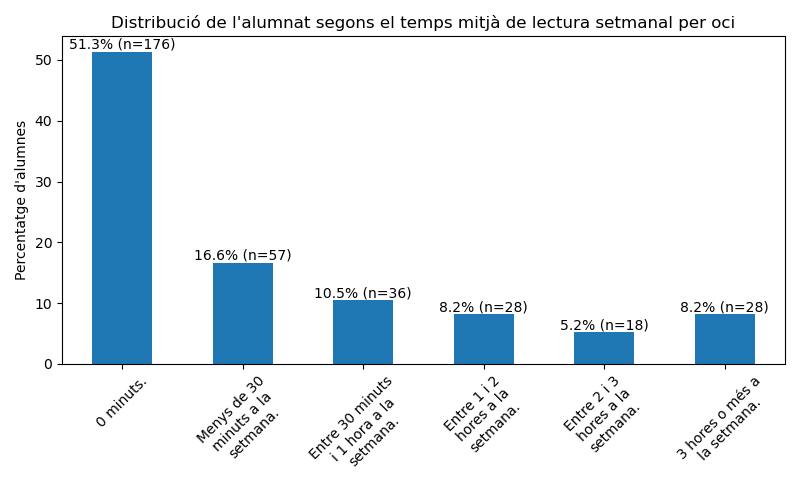
\includegraphics[width=0.85\textwidth]{pictures/2_temps.png}
    \caption{Distribució de l'alumnat segons el temps mitjà de lectura setmanal de llibres o còmics per oci.}
    \label{fig:temps}
\end{figure}

Pel que fa al nombre de llibres o còmics llegits durant els darrers 12 mesos (\autoref{fig:llibres}), observem que el 35.3\% ($n =$ 121) de l’alumnat no n’ha llegit cap, i el 61.2\% ($n = 210$) n’ha llegit com a màxim dos. En canvi, només el 19.5\% ($n =$ 67) afirma haver llegit més de cinc llibres o còmics durant aquest període.

\begin{figure}[H]
    \centering
    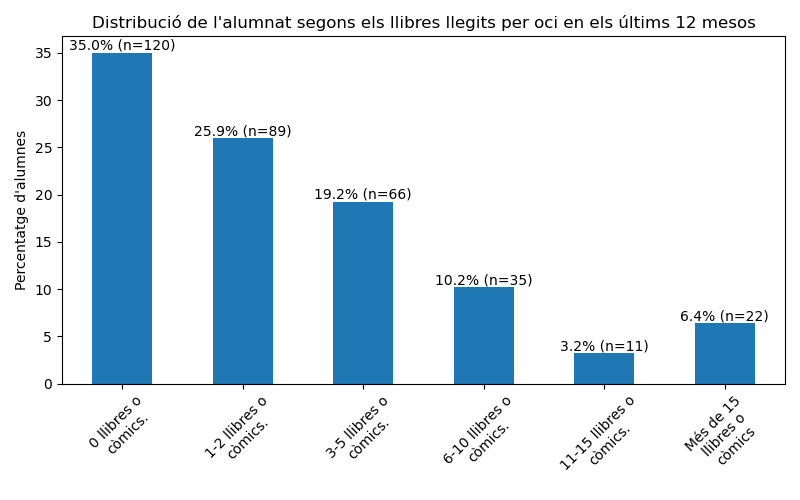
\includegraphics[width=0.85\textwidth]{pictures/2_llibres.png}
    \caption{Distribució de l'alumnat segons el nombre de llibres o còmics llegits en els últims 12 mesos per oci.}
    \label{fig:llibres}
\end{figure}

La distribució observada tant en el temps mitjà dedicat a la lectura de llibres o còmics setmanalment per oci, com en el nombre de llibres o còmics llegits durant els darrers 12 mesos per oci, presenta una tendència similar. Aquest fet és coherent amb l’elevada correlació de Spearman observada entre ambdues variables ($\rho =$ .0.860, p < .001).

\subsubsection{Resultats temps mitjà de lectura setmanal i llibres o còmics llegits en els últims 12 mesos per oci per gènere} \label{sec:resus_genere}
Per a les anàlisis inferencials relacionades amb el gènere, s’ha exclòs la categoria ``prefereixo no respondre'' a causa del reduït nombre de casos ($n =$ 9, 2.6\%) presents en aquesta categoria, tal com s'observa a la \autoref{fig:descriptive_genere}.

Els resultats obtinguts en funció del gènere ens mostren diferències clares entre nois i noies. Tal com s'observa a la \autoref{fig:temps_genere}, els nois presenten una proporció més elevada d’alumnes que no dedica, o dedica poc temps, de mitjana, a la lectura de llibres o còmics per oci setmanalment: un 55.8\% dels nois no dedica, de mitjana, cap minut setmanal a aquesta activitat, i un 73.7\% li dedica menys de 30 minuts, enfront del 47.2\% i 61.8\% de les noies, respectivament.

D’altra banda, les noies mostren una major presència en les categories de lectura més freqüent: el 7.9\% de les noies dedica entre 2 i 3 hores setmanals, de mitjana, a la lectura de llibres o còmics per oci (en comparació amb el 2.6\% dels nois), i el 12.4\% de les noies dedica més de 3 hores setmanals, de mitjana, a aquesta activitat (en comparació amb el 3.8\% dels nois).

\begin{figure}[H]
    \centering
    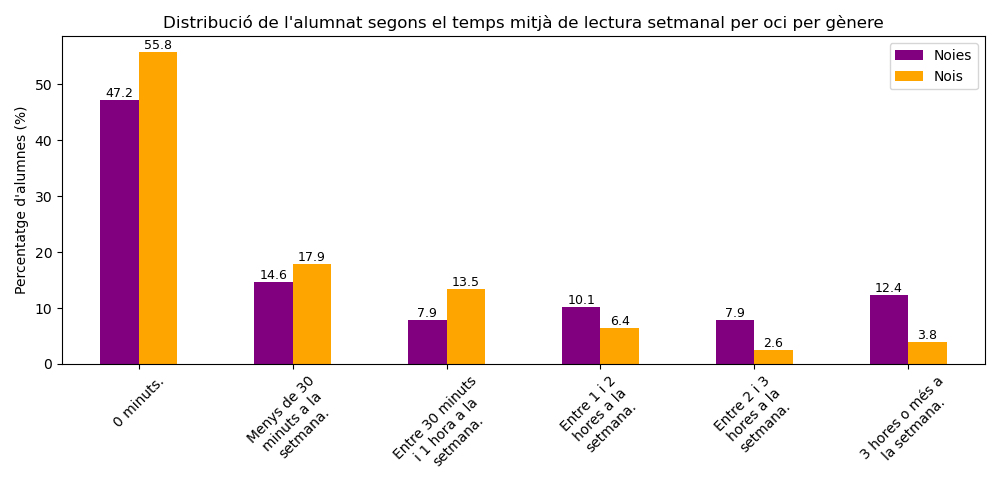
\includegraphics[width=\textwidth]{pictures/2_temps_genere.png}
    \caption{Distribució de l'alumnat segons el temps mitjà setmanal dedicat a la lectura de llibres o còmics per oci per gènere.}
    \label{fig:temps_genere}
\end{figure}

Aquesta tendència també s’observa a la \autoref{fig:llibres_genere}, que representa el nombre de llibres o còmics llegits durant els darrers 12 mesos per oci en funció del gènere. Un 42.9\% dels nois no ha llegit cap llibre o còmic per oci en l'últim any, respecte d'un 28.1\% de les noies. Tanmateix, les noies concentren percentatges superiors en les categories de lectura més elevades, especialment entre 6 i 10 llibres o còmics anuals (13.5\% envers el 7.1\% dels nois) i en més de 10 llibres (12.4\% envers el 6.4\% dels nois).

\begin{figure}[H]
    \centering
    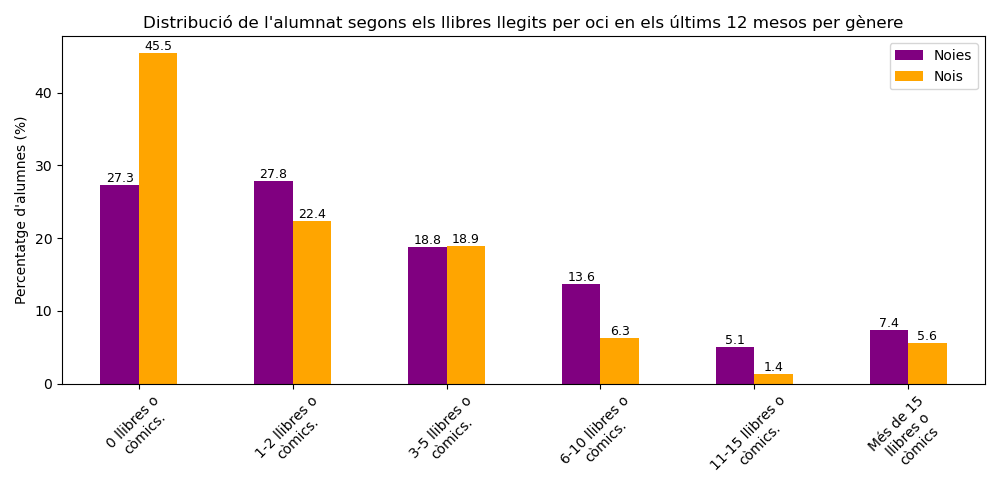
\includegraphics[width=\textwidth]{pictures/2_llibres_genere.png}
    \caption{Distribució de l'alumnat segons el nombre de llibres o còmics llegits en els últims 12 mesos per oci per gènere.}
    \label{fig:llibres_genere}
\end{figure}

La prova $\chi^2$ d’independència confirma una associació estadísticament significativa entre el gènere i tant el temps setmanal dedicat a la lectura per oci ($\chi^2 = 17.136$, $p = .004$) com el nombre de llibres o còmics llegits durant els darrers 12 mesos ($\chi^2 = 13.289$, $p = .021$). Tanmateix, els valors del coeficient V de Cramér indiquen que aquestes associacions són de baixa intensitat (V = .227 i V = .199, respectivament).

\subsubsection{Resultats temps mitjà de lectura setmanal i llibres o còmics llegits en els últims 12 mesos per oci per curs i per itinerari de batxillerat} \label{sec:lec_curs}
Quant al curs acadèmic i a l’itinerari de batxillerat, no s’observen diferències clares ni consistents en els hàbits de lectura per oci. En el cas del curs, no es detecta una tendència evolutiva entre nivells educatius, tot i que 4t d’ESO concentra els percentatges més elevats d’alumnat amb menor dedicació a la lectura, tant en temps setmanal com en nombre de llibres llegits. Pel que fa a l’itinerari, no s’identifiquen diferències rellevants entre l’alumnat de Ciències Socials i el de Ciències i Tecnologia.

Les distribucions completes es poden consultar a la \autoref{graf:descript_llibres_temps}.

\subsection{Nombre estimat de pàgines anuals llegides per oci per grups} \label{sec:pagines_grups}
% ---------------------------------------------------
\subsubsection{Resultats generals de pàgines anuals estimades llegides per oci}
Pel que fa a la distribució de la variable de pàgines estimades llegides anualment de llibres o còmics per oci (\autoref{tab:estadistiques_descriptives}), s’observa una forta asimetria positiva, deguda, com s’ha evidenciat anteriorment, a l’elevada proporció d’alumnes que no ha llegit cap llibre o còmic per oci durant els darrers 12 mesos. Aquest fet es reflecteix en la discrepància notable entre la mitjana ($\bar{x}$ = 1190.60 pàgines) i la mediana ($Q_2$ = 300 pàgines), indicant que la major part de l’alumnat ha llegit molt poques pàgines de llibres o còmics per oci aquest últim any, mentre que un petit grup d’estudiants ha llegit un volum considerable.

\begin{table}[H]
\centering
\begin{tabular}{lr}
\hline
\textbf{Estadístics} & \textbf{Valor} \\
\hline
$n$ & 343 \\
$\bar{x}$ & 1190.60 \\
$s$ & 2143.86 \\
$\min(x)$ & 0 \\
$Q_1$ & 0 \\
$Q_2$ (mediana) & 300 \\
$Q_3$ & 800 \\
$\max(x)$ & 12600 \\
\hline
\end{tabular}
\vspace{0.5em}
\caption{Estadístics de la variable nombre de pàgines estimades llegides de llibres o còmics per oci en els últims 12 mesos.}
\label{tab:estadistiques_descriptives}
\end{table}

Aquesta asimetria es posa també de manifest en la gran quantitat d'\emph{outliers} (valors atípics) en el rang superior de la distribució que s'observen en el \emph{boxplot} de la \autoref{fig:pagines_boxplot}. Aquests valors extrems contribueixen a ampliar la dispersió global de la variable ($s$ = 2143.86), la qual concentra un gran nombre de casos en el rang baix de pàgines estimades llegides, alhora que uns pocs casos presenten valors molt elevats, arribant fins a un màxim de 12.600 pàgines anuals.

\begin{figure}[H]
    \centering
    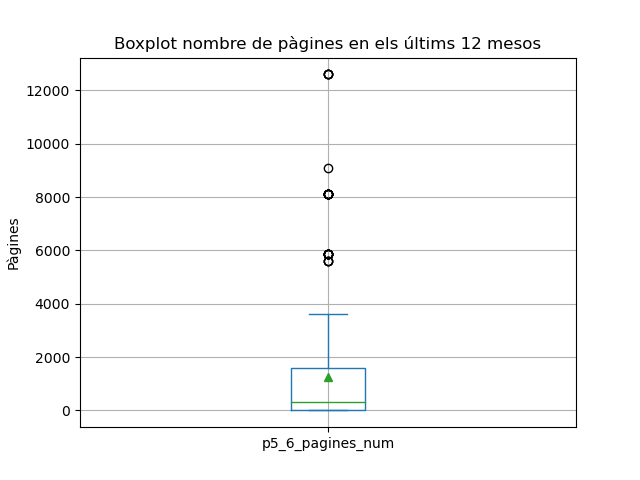
\includegraphics[width=0.7\textwidth]{pictures/3_pagines_boxplot.png}
    \caption{\emph{Boxplot} de la variable nombre de pàgines estimades llegides de llibres o còmics per oci en els últims 12 mesos.}
    \label{fig:pagines_boxplot}
\end{figure}

\subsubsection{Resultats de pàgines anuals estimades llegides per oci per gènere} \label{sec:pagines_genere}

Considerant la distribució de la variable de pàgines estimades llegides anualment per oci en funció del gènere (\autoref{tab:estadistics_pagines_genere}), s’observen diferències clares i consistents entre ambdós grups dominants. En primer lloc, les noies presenten valors substancialment superiors en tots els estadístics de tendència central, amb una mitjana $\bar{x}$ = 1632.30 pàgines, envers $\bar{x}$ = 727.88 en el cas dels nois. La mediana de pàgines estimades llegides també és notablement més elevada per les noies $Q_2$ = 675, que pels nois $Q_2$ = 250. 

\begin{table}[H]
\centering
\begin{tabular}{lrr}
\hline
\textbf{Estadístics} & \textbf{Femení} & \textbf{Masculí} \\
\hline
$n$ & 178 & 156 \\
$\bar{x}$ & 1632.30 & 727.88 \\
$s$ & 2564.33 & 1456.02 \\
$\min(x)$ & 0 & 0 \\
$Q_1$ & 0 & 0 \\
$Q_2$ (mediana) & 675 & 250 \\
$Q_3$ & 1800 & 800 \\
$\max(x)$ & 12600 & 8100 \\
\hline
\end{tabular}
\vspace{0.5em}
\caption{Estadístics descriptius de la variable pàgines estimades llegides anualment per oci en funció del gènere.}
\label{tab:estadistics_pagines_genere}
\end{table}

Aquestes diferències estadístiques ens mostren com el volum de lectura per oci és considerablement més elevat en les noies que en els nois, resultat que concorda amb l'esmentat en l'apartat anterior: \nameref{sec:resus_genere}.

Per ambdós gèneres s’observa una marcada asimetria positiva en la distribució del nombre de pàgines llegides, la qual indica que la majoria d’estudiants llegeix poc o molt poc per oci, mentre que un petit grup concentra valors molt elevats. Aquesta dispersió és més pronunciada en el cas de les noies, que presenten mesures de dispersió més elevades ($s$ = 2564.33, envers $s$ = 1456.02 els nois) i una major quantitat d'\emph{outliers} (\autoref{fig:pagines_boxplot_genere}).

\begin{figure}[H]
    \centering
    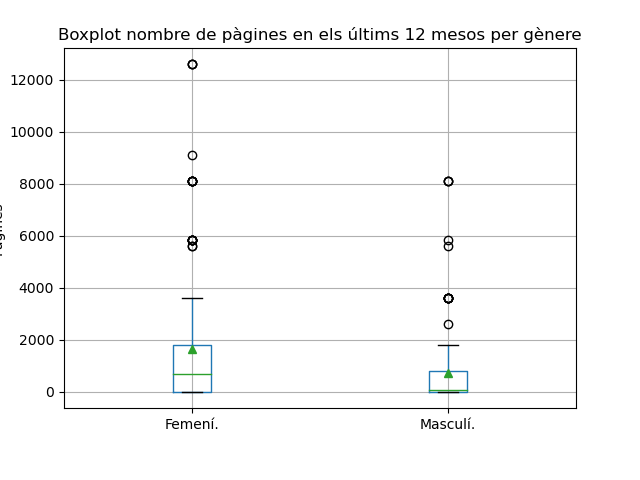
\includegraphics[width=0.8\textwidth]{pictures/3_pagines_boxplot_genere.png}
    \caption{\emph{Boxplots} de la variable nombre de pàgines estimades llegides de llibres o còmics per oci en els últims 12 mesos en funció del gènere.}
    \label{fig:pagines_boxplot_genere}
\end{figure}

\subsubsection{Resultats de pàgines anuals llegides per oci per curs}\label{sec:pagines_curs}
En relació amb la distribució de la variable de pàgines estimades llegides anualment per oci en funció del curs acadèmic, no s’observa un patró lineal clar de variació a mesura que s’avança en l’etapa educativa.

En aquest sentit, els estadístics descriptius de la \autoref{tab:estadistics_pagines_curs} mostren valors relativament similars entre la majoria dels cursos, fet que suggereix una variabilitat limitada en el volum de lectura entre nivells educatius. L’única excepció destacable és 4t d’ESO, que presenta els valors més baixos, tant en termes de mitjana ($\bar{x}$ = 437.16 pàgines), com de mediana ($Q_2$ = 250 pàgines), indicant un volum de lectura especialment reduït. En aquest curs, tampoc hi ha estudiants que presentin volums de pàgines tan elevats com en altres cursos, fet que es reflecteix en la menor dispersió de la variable ($s$ = 664.19).

\begin{table}[H]
\centering
\begin{tabular}{lrrrrrrrr}
\hline
\textbf{Estadístics} & \textbf{3r ESO} & \textbf{4t ESO} & \textbf{1r Batx.} & \textbf{2n Batx.} \\
\hline
$n$ & 110 & 74 & 86 & 73 \\
$\bar{x}$ & 1535.00 & 437.16 & 1158.43 & 1473.29 \\
$s$ & 2667.76 & 664.19 & 1913.62 & 2332.41 \\
$\min(x)$ & 0 & 0 & 0 & 0 \\
$Q_1$ & 0 & 0 & 0 & 0 \\
$Q_2$ (mediana) & 300 & 250 & 300 & 300 \\
$Q_3$ & 1600 & 675 & 800 & 1800 \\
$\max(x)$ & 12600 & 3600 & 8100 & 12600 \\
\hline
\end{tabular}
\vspace{0.5em}
\caption{Estadístics descriptius de la variable pàgines estimades llegides anualment per oci en funció del curs acadèmic.}
\label{tab:estadistics_pagines_curs}
\end{table}

Quant a l'itinerari de batxillerat, no s'observen diferències rellevants entre l'alumnat de Ciències Socials i el de Ciències i Tecnologia. La taula completa es troba a la \autoref{graf:descript_pag}.

\subsection{Classificació lectora per oci}
% ---------------------------------------------------

La distribució de la variable \emph{classificació lectora per oci} (\autoref{fig:classificacio}) mostra que la major part de l’alumnat es concentra en la categoria de \emph{no lector / lector molt ocasional} (69.1\%), mentre que només un 17.2\% pertany a la categoria \emph{lector habitual}. Aquest patró és coherent amb els resultats descriptius presentats en l'apartat \nameref{sec:results_gen}, que evidencien una elevada proporció d’alumnes amb nivells baixos o nuls de lectura de llibres o còmics per oci.

\begin{figure}[H]
    \centering
    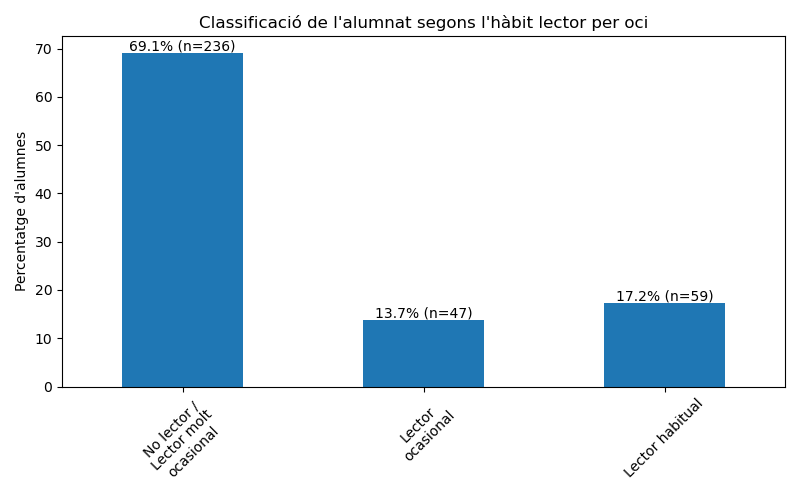
\includegraphics[width=0.8\textwidth]{pictures/4_class.png}
    \caption{Classificació de l'alumnat segons l'hàbit lector per oci.}
    \label{fig:classificacio}
\end{figure}

Respecte al gènere (\autoref{fig:classificacio_genere}), els resultats mantenen la tendència observada en les anàlisis prèvies (\nameref{sec:resus_genere}; \nameref{sec:pagines_genere}): els nois presenten un percentatge superior en la categoria de \emph{no lector / lector molt ocasional} (75.0\%) en comparació amb les noies (62.9\%), mentre que les noies concentren una major proporció de \emph{lectores habituals} per oci (25.3\% davant del 9.0\% en els nois).

\begin{figure}[H]
    \centering
    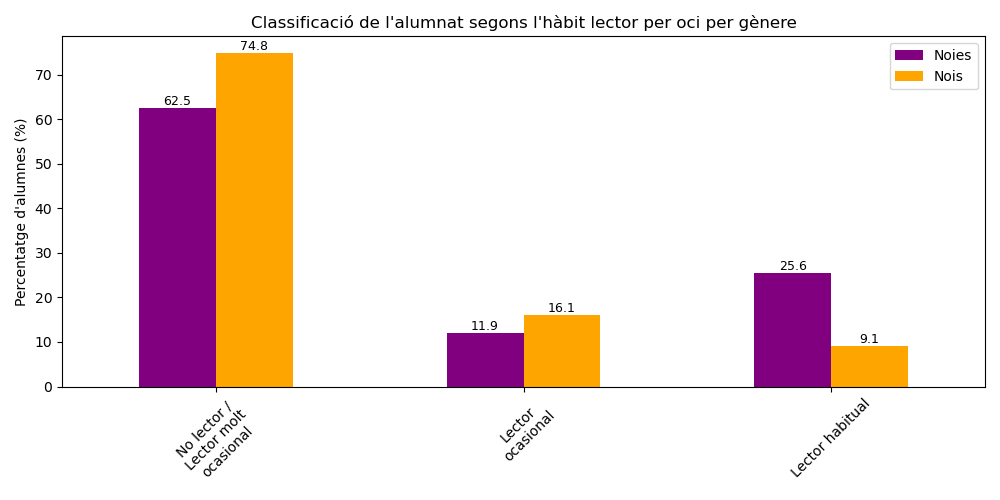
\includegraphics[width=\textwidth]{pictures/4_class_genere.png}
    \caption{Classificació de l'alumnat segons l'hàbit lector per oci per gènere.}
    \label{fig:classificacio_genere}
\end{figure}

En funció del curs acadèmic (\autoref{fig:classificacio_curs}), tampoc no s’observa una tendència lineal clara, tot i que 4t d’ESO destaca novament com el curs amb una major concentració d’alumnat en la categoria de \emph{no lector / lector molt ocasional} (82.4\%) i una menor proporció de \emph{lectors habituals} (5.4\%), reforçant els patrons observats en els apartats \nameref{sec:lec_curs}, i \nameref{sec:pagines_curs}.

\begin{figure}[H]
    \centering
    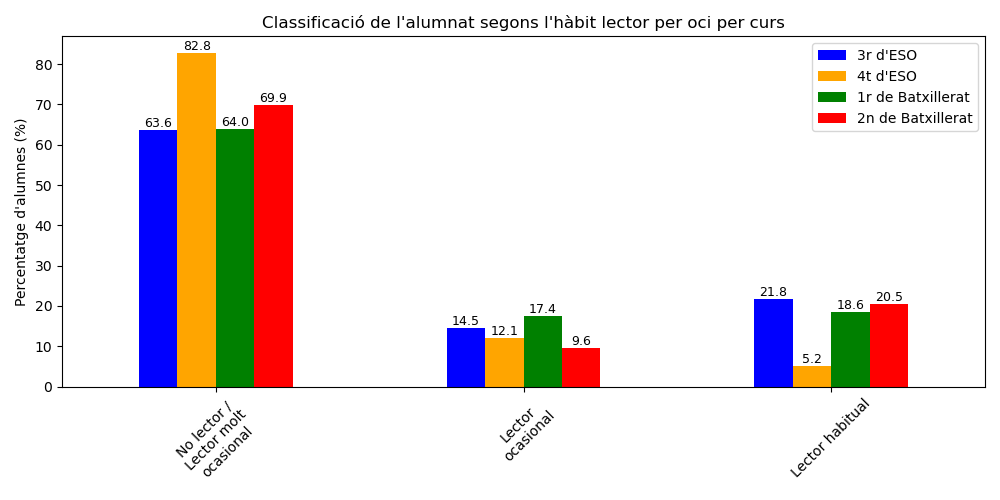
\includegraphics[width=\textwidth]{pictures/4_class_curs.png}
    \caption{Classificació de l'alumnat segons l'hàbit lector per oci per curs.}
    \label{fig:classificacio_curs}
\end{figure}

\subsection{Temàtica i format preferits per a la lectura per oci}
% ---------------------------------------------------

Observant els resultats obtinguts pel conjunt de la mostra (\autoref{fig:ranking_thematic}), la novel·la romàntica, la novel·la fantàstica i el còmic són les categories que més es llegeixen per oci; i poesia i teatre les que menys. Tanmateix, hi ha diferències considerables en funció del gènere (\autoref{fig:ranking_thematic_girls} i \autoref{fig:ranking_thematic_boys}): les noies presenten una preferència especialment marcada per la novel·la romàntica, seguida de la novel·la fantàstica i el còmic, mentre que els nois mostren una distribució més equilibrada entre diferents gèneres, amb una presència destacable del còmic, la novel·la fantàstica i la ciència-ficció.

\begin{figure}[H]
    \centering
    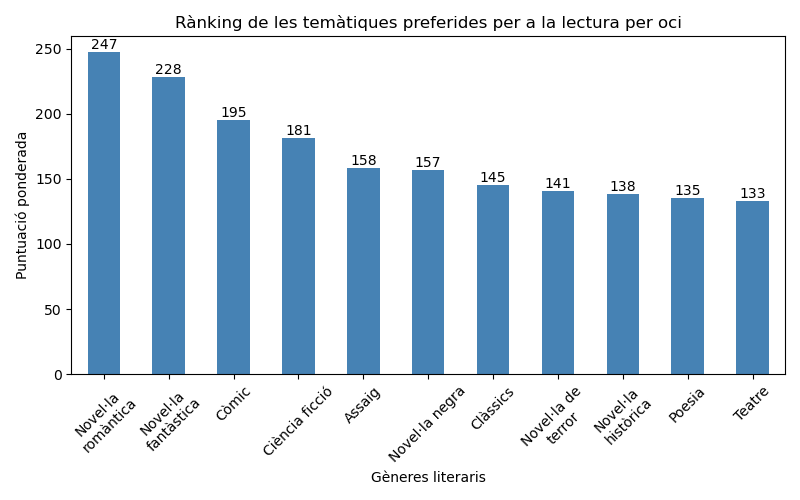
\includegraphics[width=\textwidth]{pictures/5_thematic.png}
    \caption{Rànking de les temàtiques preferides per a la lectura per oci.}
    \label{fig:ranking_thematic}
\end{figure}

\begin{figure}[H]
    \centering
    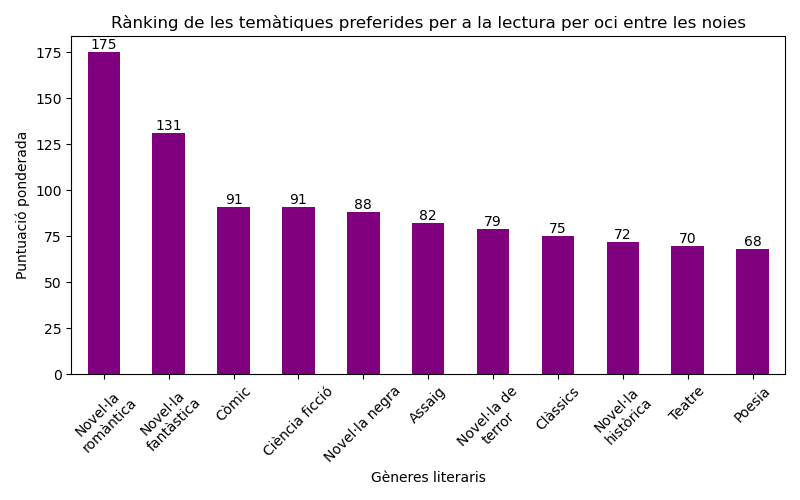
\includegraphics[width=\textwidth]{pictures/5_thematic_girls.png}
    \caption{Rànking de les temàtiques preferides per a la lectura per oci entre les noies.}
    \label{fig:ranking_thematic_girls}
\end{figure}

\begin{figure}[H]
    \centering
    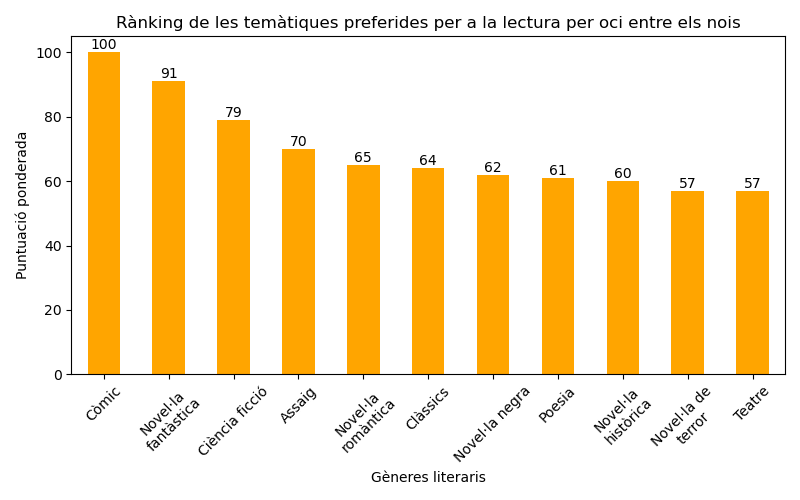
\includegraphics[width=\textwidth]{pictures/5_thematic_boys.png}
    \caption{Rànking de les temàtiques preferides per a la lectura per oci entre els nois.}
    \label{fig:ranking_thematic_boys}
\end{figure}

Pel que fa al format de lectura (\autoref{fig:ranking_format}), s’observa un predomini molt clar del format físic o en paper, utilitzat pel 88.4\% de l’alumnat que llegeix per oci. En comparació, els formats digitals presenten una presència considerablement menor, tant en dispositius web o PDF (8.2\%) com en format \emph{ebook} (3.4\%).

\begin{figure}[H]
    \centering
    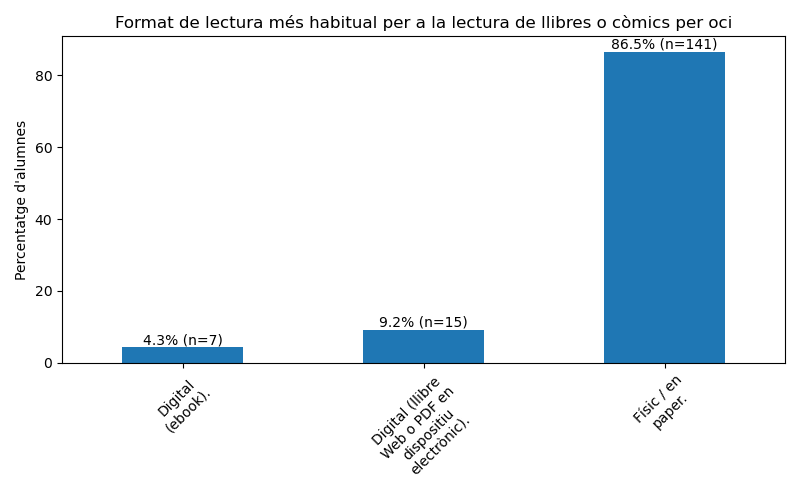
\includegraphics[width=0.85\textwidth]{pictures/5_format.png}
    \caption{Format de lectura preferit per a la lectura per oci de llibres o còmics.}
    \label{fig:ranking_format}
\end{figure}

\subsection{Lectura per oci i sessions de lectura}
% ---------------------------------------------------

\subsubsection{Resultats durada sessions de lectura}
Quant a la durada de les sessions de lectura per oci (\autoref{fig:tipologia_sessions}), s’observa com una part important de l’alumnat que llegeix per oci afirma no seguir un patró clar o estable de lectura (35.9\%, $n = 84$), mentre que només una minoria declara realitzar sessions gairebé sempre molt curtes inferiors als 15 minuts (8.5\%, $n = 20$).

\begin{figure}[H]
    \centering
    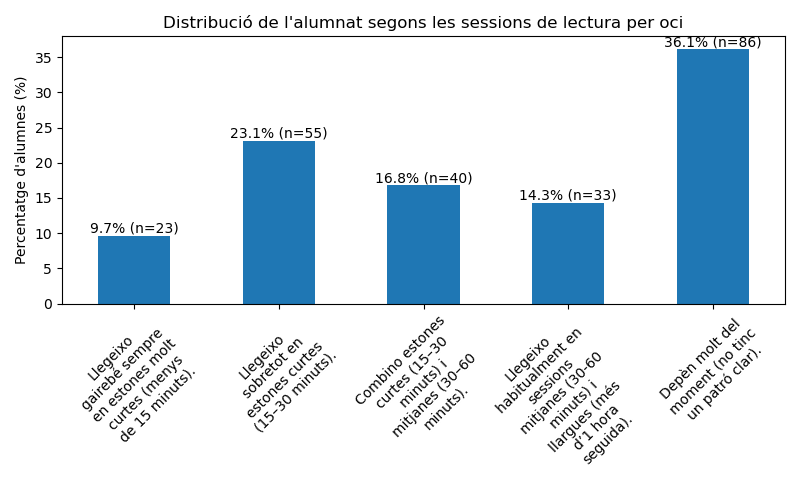
\includegraphics[width=0.85\textwidth]{pictures/6_sessions.png}
    \caption{Distribució de l'alumnat segons la durada de les sessions de lectura per oci.}
    \label{fig:tipologia_sessions}
\end{figure}

En funció de la classificació lectora (\autoref{fig:tipologia_sessions_class}), els no lectors o lectors molt ocasionals concentren percentatges més elevats en les categories de sessions curtes, mentre que els lectors ocasionals i, especialment, els lectors habituals presenten una proporció més elevada de sessions de lectura mitjanes i llargues.

\begin{figure}[H]
    \centering
    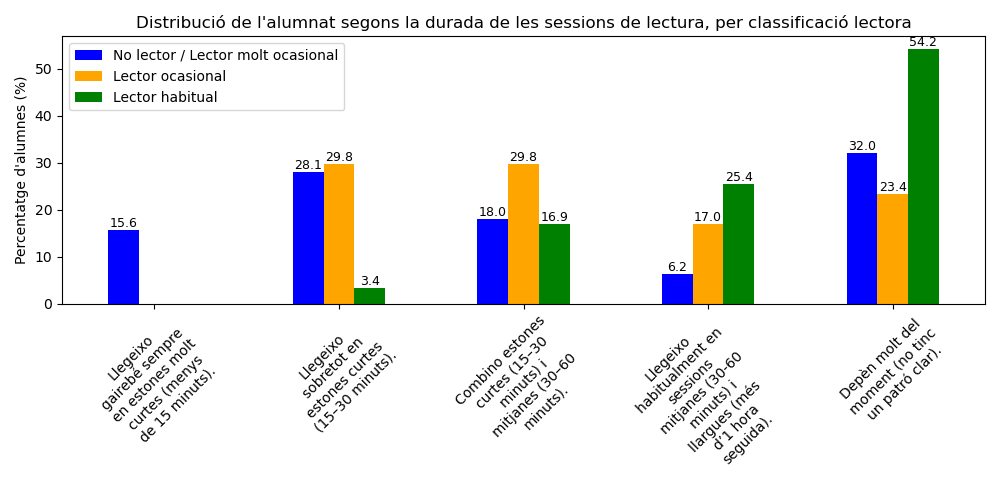
\includegraphics[width=\textwidth]{pictures/6_sessions_class.png}
    \caption{Distribució de l'alumnat segons la durada de les sessions de lectura per oci, per classificació lectora.}
    \label{fig:tipologia_sessions_class}
\end{figure}

Aquesta relació es veu reforçada per les correlacions positives moderades observades entre la durada de les sessions de lectura per oci, i, tant el temps mitjà setmanal dedicat a la lectura per oci ($\rho = .502$, $p < .001$), com el nombre de llibres llegits anualment per oci ($\rho = .491$, $p < .001$).

Cal esmentar que, aquestes correlacions s'han calculat excloent els casos que no segueixen un patró clar de lectura, ja que aquesta categoria no proporciona informació específica sobre la durada de les sessions i podria distorsionar la relació entre les variables.

\subsubsection{Resultats consulta de xarxes socials mentre llegeixen}
Pel que fa a la freqüència de consulta de xarxes socials durant la lectura (\autoref{fig:tipologia_consulta_xs}), destaca l'alt percentatge d'alumnes que afirma no consultar les xarxes socials mentre llegeix (35\%, $n = 120$), i l'alt percentatge que també afirma consultar-les aproximadament cada 15 minuts o menys (35\%, $n = 120$).

\begin{figure}[H]
    \centering
    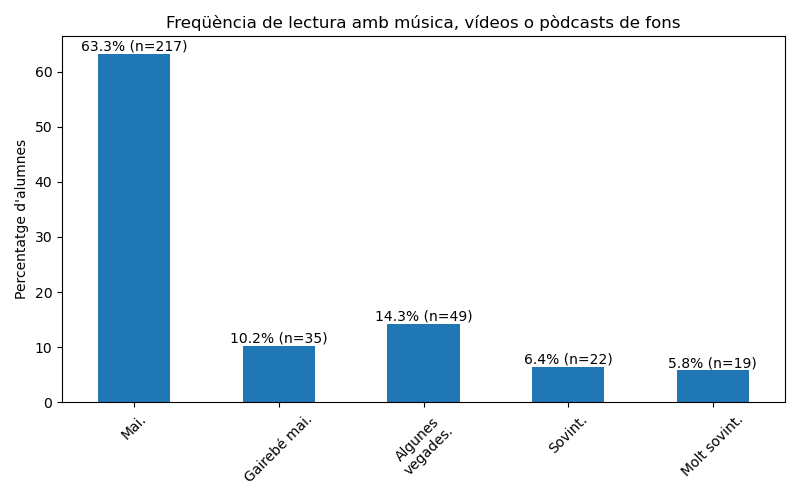
\includegraphics[width=0.85\textwidth]{pictures/6_consulta_xs.png}
    \caption{Distribució de l'alumnat segons la freqüència de consulta de xarxes socials durant la lectura.}
    \label{fig:tipologia_consulta_xs}
\end{figure}

Analitzant els resultats en funció de la classificació lectora (\autoref{fig:tipologia_consulta_xs_class}), es poden observar diferències rellevants entre els diferents perfils. En el cas dels no lectors o lectors molt ocasionals, una proporció més elevada consulta les xarxes socials mentre llegeix cada menys de 15 minuts (47.3\%), respecte al 14.9\% dels lectors ocasionals i al 1.7\% dels lectors habituals. D'altra banda, la proporció d’alumnes que no acostuma a consultar les xarxes socials durant la lectura és més baixa en el grup dels no lectors o lectors molt ocasionals (23.6\%) en comparació amb els lectors ocasionals (59.6\%) i els lectors habituals (61\%).

\begin{figure}[H]
    \centering
    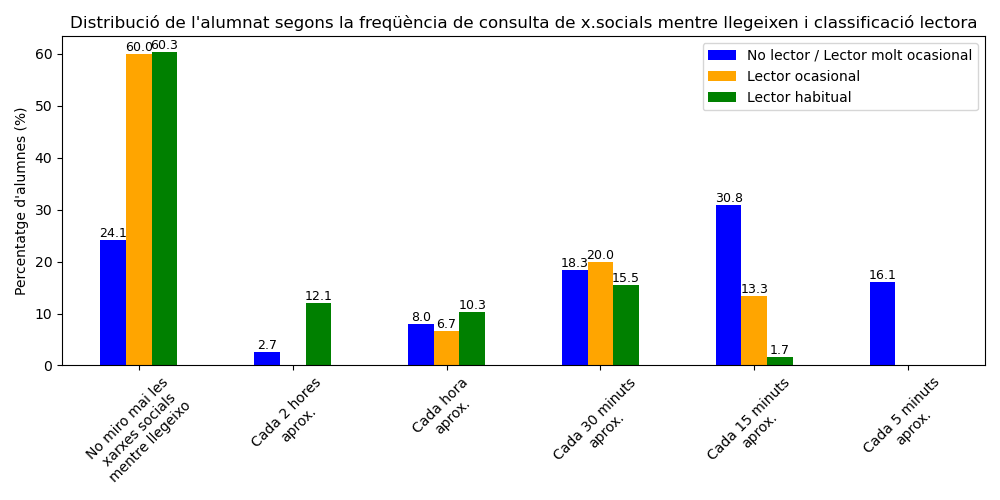
\includegraphics[width=\textwidth]{pictures/6_consulta_xs_class.png}
    \caption{Distribució de l'alumnat segons la freqüència de consulta de xarxes socials durant la lectura, per classificació lectora.}
    \label{fig:tipologia_consulta_xs_class}
\end{figure}

En sintonia, s’observen correlacions negatives moderades entre la consulta de xarxes socials durant la lectura i el temps mitjà de lectura setmanal per oci ($\rho = -.385$, $p < .001$), així com amb el nombre de llibres llegits anualment per oci ($\rho = -.416$, $p < .001$). De manera coherent, també es detecta una correlació negativa feble entre la freqüència de consulta de xarxes socials i la durada de les sessions de lectura ($\rho = -.312$, $p < .001$).

\subsubsection{Resultats escolta de música, vídeos o pòdcasts durant la lectura}
En relació amb la freqüència d'escoltar música, vídeos o pòdcasts de fons durant la lectura (\autoref{fig:tipologia_musica}), els resultats mostren que la major part de l’alumnat no acostuma a fer-ho (63.3\%), mentre que només una petita part afirma fer-ho sovint o molt sovint (12.2\%).

\begin{figure}[H]
    \centering
    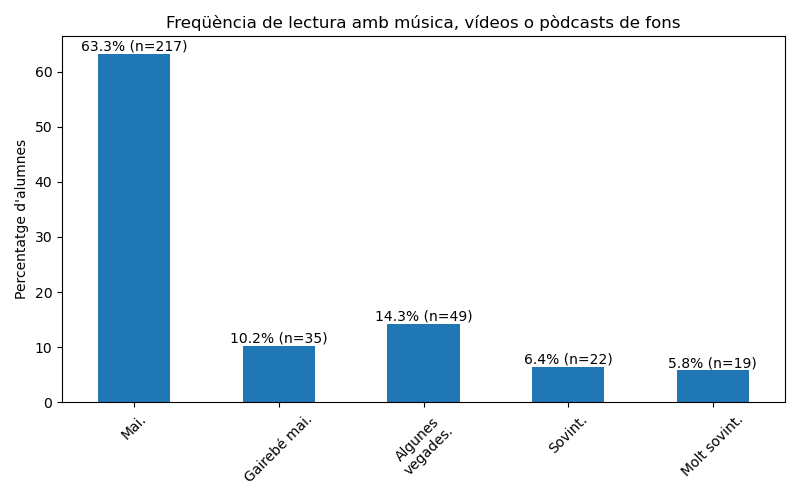
\includegraphics[width=0.85\textwidth]{pictures/6_musica.png}
    \caption{Distribució de l'alumnat segons la freqüència amb la que escolten música, vídeos o pòdcasts de fons mentre llegeixen.}
    \label{fig:tipologia_musica}
\end{figure}

Analitzant els resultats en funció de la classificació lectora (\autoref{fig:tipologia_musica_class}), inicialment s’observen correlacions positives molt febles amb el temps mitjà de lectura setmanal per oci ($\rho = .18$, $p < .001$) i el nombre de llibres llegits anualment per oci ($\rho = .177$, $p < .001$). Els lectors habituals presenten una subtil major proporció d’alumnes que escolta sovint o molt sovint música, vídeos o pòdcasts de fons mentre llegeix (18.7\%) respecte als lectors ocasionals (10.6\%) i als no lectors o lectors molt ocasionals (11\%).

Tanmateix, aquestes correlacions positives perden completament la significació estadística quan l’anàlisi es restringeix únicament a l’alumnat que llegeix per oci ($p = 0.093$ respecte al temps mitjà de lectura setmanal; $p = 0.119$ respecte al nombre de llibres llegits anualment).

\begin{figure}[H]
    \centering
    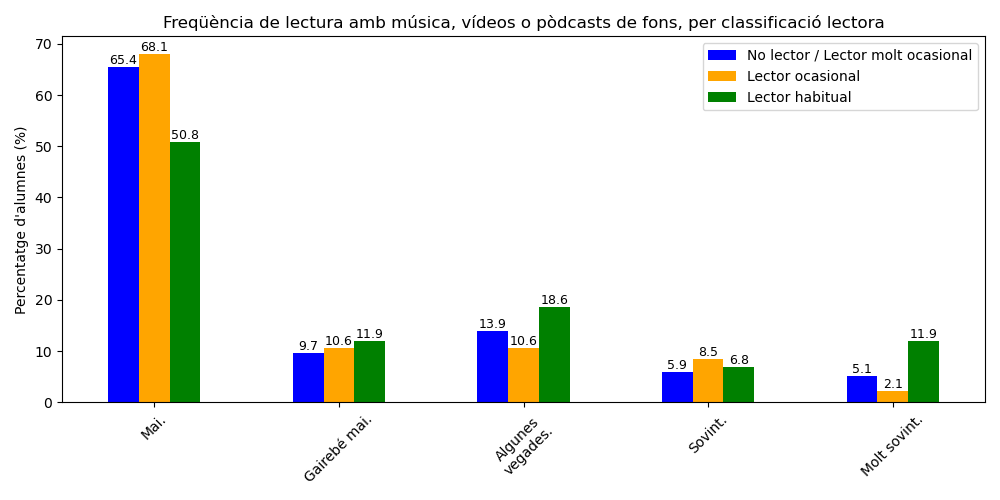
\includegraphics[width=\textwidth]{pictures/6_musica_class.png}
    \caption{Distribució de l'alumnat segons la freqüència amb la que escolten música, vídeos o pòdcasts de fons mentre llegeixen, per classificació lectora.}
    \label{fig:tipologia_musica_class}
\end{figure}

\subsection{Lectura per oci i visites a la biblioteca}
% ---------------------------------------------------
En relació amb les visites a la biblioteca per agafar llibres o còmics en préstec durant l’últim any (\autoref{fig:tipologia_biblio}), el 67.3\% de l'alumnat declara no haver anat cap vegada a la biblioteca amb aquesta finalitat durant l’últim any, mentre que només una petita proporció d’alumnes (11.7\%) hi ha anat més de tres vegades.

\begin{figure}[H]
    \centering
    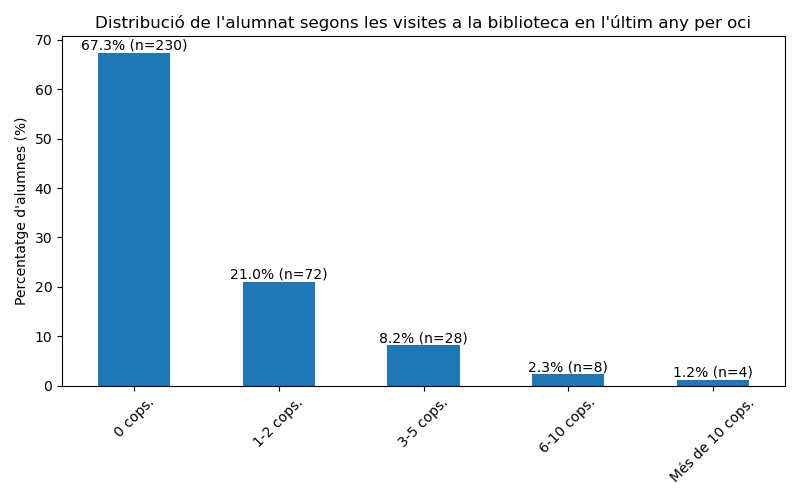
\includegraphics[width=0.85\textwidth]{pictures/7_biblio.png}
    \caption{Distribució de l'alumnat segons la freqüència amb la que han visitat la biblioteca l'últim any.}
    \label{fig:tipologia_biblio}
\end{figure}

Tanmateix, s’observen diferències rellevants en funció de la classificació lectora (\autoref{fig:tipologia_biblio_class}). Els lectors habituals presenten una proporció més elevada d’alumnes que ha visitat la biblioteca més de tres vegades durant l’últim any per agafar llibres o còmics en préstec (21.7\%), respecte als lectors ocasionals (17\%) i als no lectors o lectors molt ocasionals (6.8\%). D’altra banda, els no lectors o lectors molt ocasionals concentren la proporció més elevada d’alumnat que no ha visitat la biblioteca cap vegada durant l’últim any amb aquesta finalitat (75.9\%), davant del 48.9\% dels lectors ocasionals i del 47.5\% dels lectors habituals.

\begin{figure}[H]
    \centering
    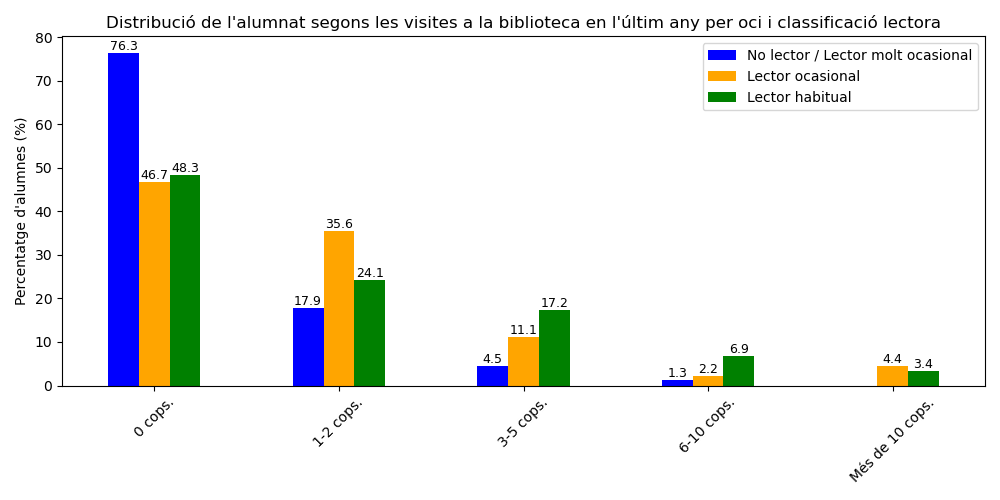
\includegraphics[width=\textwidth]{pictures/7_biblio_class.png}
    \caption{Distribució de l'alumnat segons la freqüència amb la que han visitat la biblioteca l'últim any, per classificació lectora.}
    \label{fig:tipologia_biblio_class}
\end{figure}

Aquest patró es veu reforçat per les correlacions positives febles-moderades observades entre la freqüència de visites a la biblioteca per agafar llibres o còmics en préstec durant l’últim any, i, tant el temps mitjà setmanal dedicat a la lectura per oci ($\rho = .367$, $p < .001$) com el nombre de llibres llegits anualment per oci ($\rho = .394$, $p < .001$).

En canvi, en relació amb la freqüència de visites a la biblioteca amb pares o tutors legals durant la infància i adolescència, les correlacions observades amb el temps mitjà setmanal dedicat a la lectura per oci i amb el nombre de llibres llegits anualment per oci són pràcticament negligibles ($\rho = .148$, $p = .006$ i $\rho = .117$, $p = .030$ respectivament). 

\subsection{Lectura per oci i lectures obligatories de l'escola}
% ---------------------------------------------------
Pel que fa a les lectures obligatòries, els resultats (\autoref{fig:obligatoria}) mostren que el 55.4\% de l’alumnat llegeix totes o gairebé totes les lectures obligatòries; el 21.8\% llegeix cap, poques o molt poques; i el 22.7\% llegeix aproximadament la meitat de les lectures obligatòries. 

\begin{figure}[H]
    \centering
    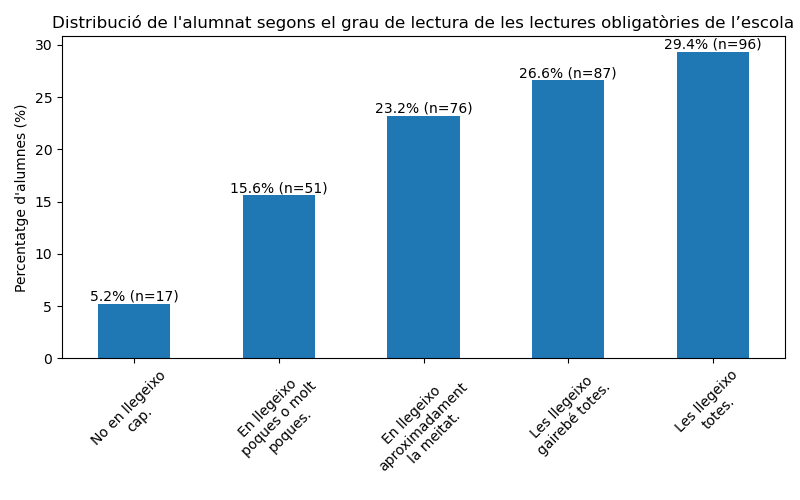
\includegraphics[width=0.85\textwidth]{pictures/8_obligatoria.png}
    \caption{Distribució de l'alumnat segons la freqüència amb la que llegeixen les lectures obligatòries.}
    \label{fig:obligatoria}
\end{figure}

Respecte a l’ús de resums d’internet o eines d’IA generativa per completar les proves associades a les lectures obligatòries (\autoref{fig:obligatoria_ia}), el 37.3\% declara utilitzar-ne sovint o molt sovint, mentre que el 31.5\% afirma no utilitzar-ne mai o gairebé mai.

\begin{figure}[H]
    \centering
    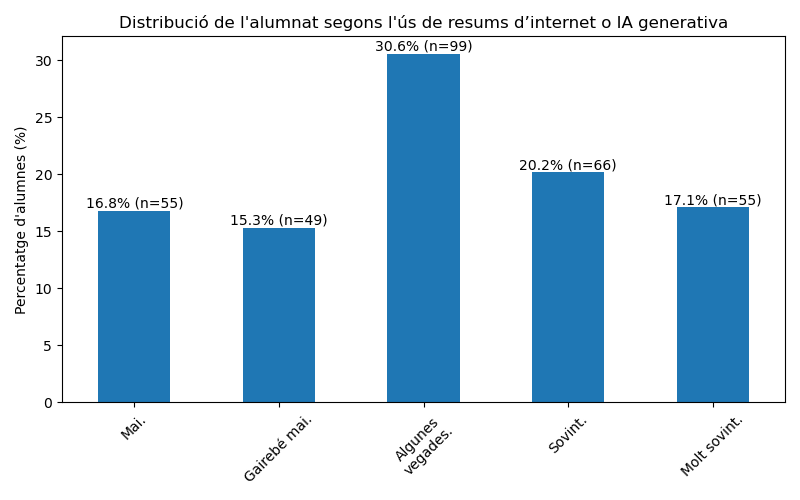
\includegraphics[width=0.85\textwidth]{pictures/8_obligatoria_ia.png}
    \caption{Distribució de l'alumnat segons la freqüència amb la que utilitzen resums d’internet o eines d’IA generativa per completar les proves associades a les lectures obligatòries.}
    \label{fig:obligatoria_ia}
\end{figure}

El grau de compromís amb les lectures obligatòries es relaciona positivament amb els hàbits lectors per oci. En concret, s’observen correlacions positives febles entre el grau de lectura de les lectures obligatòries, i, tant el temps mitjà setmanal dedicat a la lectura per oci ($\rho = .259$, $p < .001$), com el nombre de llibres llegits anualment per oci ($\rho = .299$, $p < .001$). 

Aquesta tendència també s’observa en funció de la classificació lectora (\autoref{fig:obligatoria_class}). Els lectors habituals i els lectors ocasionals presenten una proporció més elevada d’alumnes que llegeix totes les lectures obligatòries (47.5\% i 44.7\% respectivament), mentre que només el 20.7\% dels no lectors o lectors molt ocasionals afirma fer-ho. D’altra banda, els no lectors o lectors molt ocasionals concentren una major proporció d’alumnes que llegeix aproximadament la meitat o menys de les lectures obligatòries (52.4\%), respecte al 31.1\% dels lectors ocasionals i el 20.4\% dels lectors habituals.

\begin{figure}[H]
    \centering
    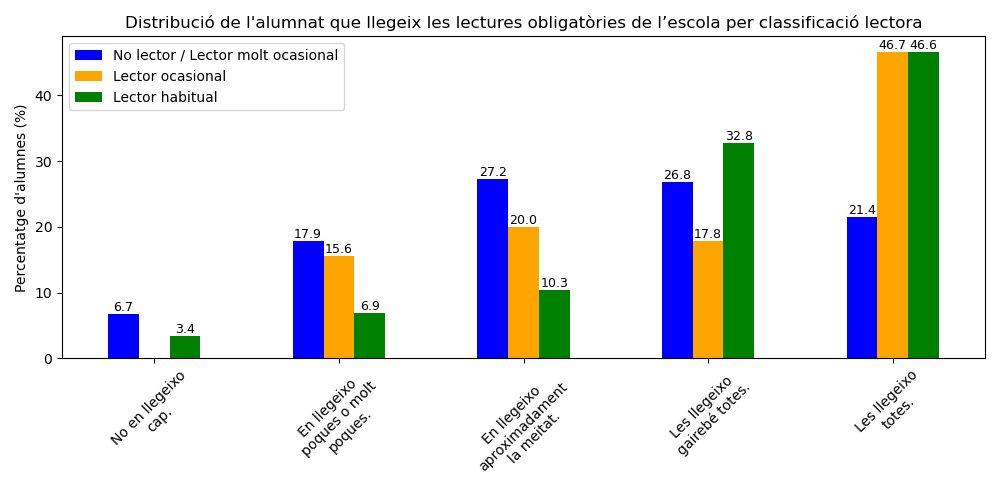
\includegraphics[width=\textwidth]{pictures/8_obligatoria_class.png}
    \caption{Distribució de l'alumnat segons la freqüència amb la que llegeixen les lectures obligatòries, per classificació lectora.}
    \label{fig:obligatoria_class}
\end{figure}

Tot i això, la valoració general de les lectures obligatòries és considerablement negativa (\autoref{fig:obligatoria_gust}). Més de la meitat de l’alumnat afirma que les lectures obligatòries els agraden ``poc'' o ``gens'' (51.3\%), mentre que només un 9.9\% declara que els agraden ``bastant'' o ``molt''. 

\begin{figure}[H]
    \centering
    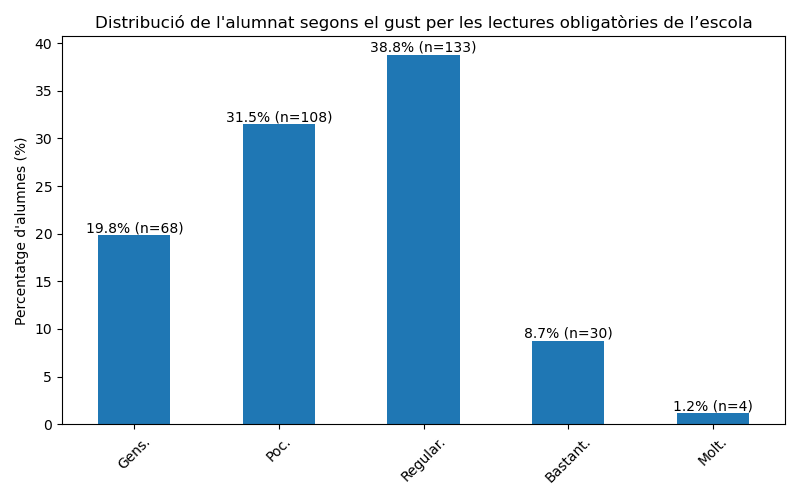
\includegraphics[width=0.85\textwidth]{pictures/8_obligatoria_gust.png}
    \caption{Distribució de l'alumnat segons el gust per les lectures obligatòries.}
    \label{fig:obligatoria_gust}
\end{figure}

De fet, el 68.8\% de l’alumnat es mostra bastant o molt d’acord amb l’afirmació que llegiria més les lectures obligatòries si aquestes s’adaptessin més als seus gustos (\autoref{fig:obligatoria_increment_gust}).

\begin{figure}[H]
    \centering
    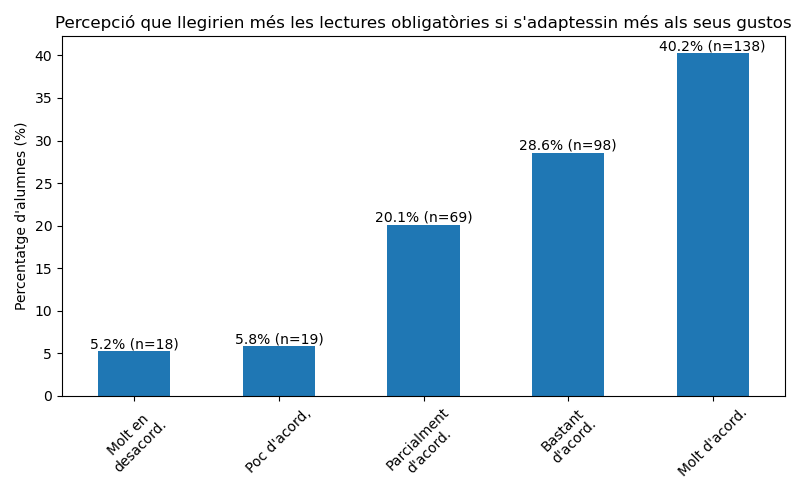
\includegraphics[width=0.85\textwidth]{pictures/8_obligatoria_increment_gust.png}
    \caption{Distribució de l'alumnat segons la percepció que llegirien més lectures obligatòries si els hi agradessin més.}
    \label{fig:obligatoria_increment_gust}
\end{figure}

En aquesta línia, s’observa una correlació positiva feble-moderada entre el gust per les lectures obligatòries i el grau de lectura d’aquestes ($\rho = .366$, $p < .001$).

% Els resultats indiquen que el gust per les lectures obligatòries presenta una relació positiva feble /molt feble amb els hàbits lectors per oci, tant pel que fa al temps mitjà setmanal dedicat a la lectura ($\rho = .237$, $p < .001$) com al nombre de llibres llegits anualment ($\rho = .175$, $p < .001$). Aquest fet suggereix que uns hàbits lectors per oci especialment consolidats no implica necessàriament una valoració més positiva de les lectures obligatòries.

% \begin{figure}[H]
%     \centering
%     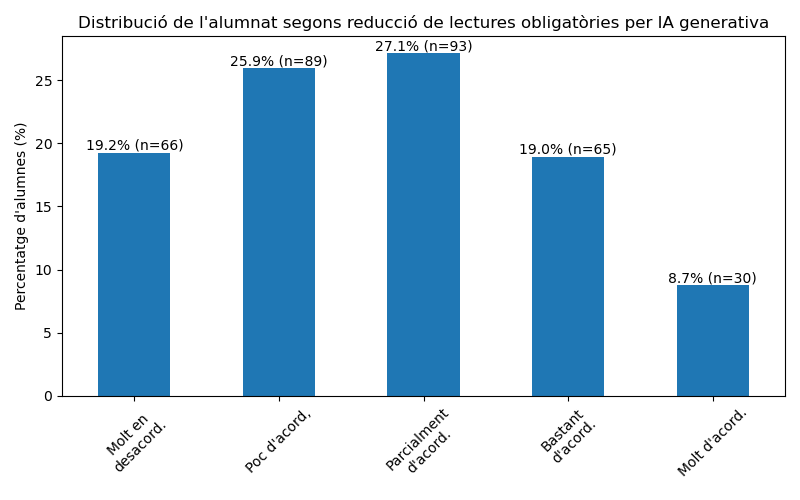
\includegraphics[width=0.85\textwidth]{pictures/8_obligatoria_reduccio.png}
%     \caption{Distribució de l'alumnat segons la reducció de lectures obligatories des que van començar a utilitzar eines d’IA generativa.}
%     \label{fig:obligatoria_reduccio}
% \end{figure}

\subsection{Lectura per oci, narrativa adolescent i percepcions personals sobre la lectura com activitat} \label{sec:narrativa}
% ---------------------------------------------------
Pel que fa a la percepció personal sobre la lectura, els resultats mostren una forta relació positiva amb els hàbits lectors per oci, tant pel que fa al temps de lectura setmanal ($\rho = .684$, $p < .001$), com al nombre de llibres llegits anualment ($\rho = .718$, $p < .001$).

Descriptivament, s'observa a la \autoref{fig:narrativa_personal_class} que els lectors habituals presenten una opinió personal sobre la lectura molt més positiva que els lectors ocasionals i els no lectors o lectors molt ocasionals. En concret, un 71.2\% dels lectors habituals percep la lectura com una activitat molt interessant i molt positiva, mentre que només el 17.0\% dels lectors ocasionals, i el 3.4\% del no lectors o lectors molt ocasionals comparteix aquesta percepció.

\begin{figure}[H]
    \centering
    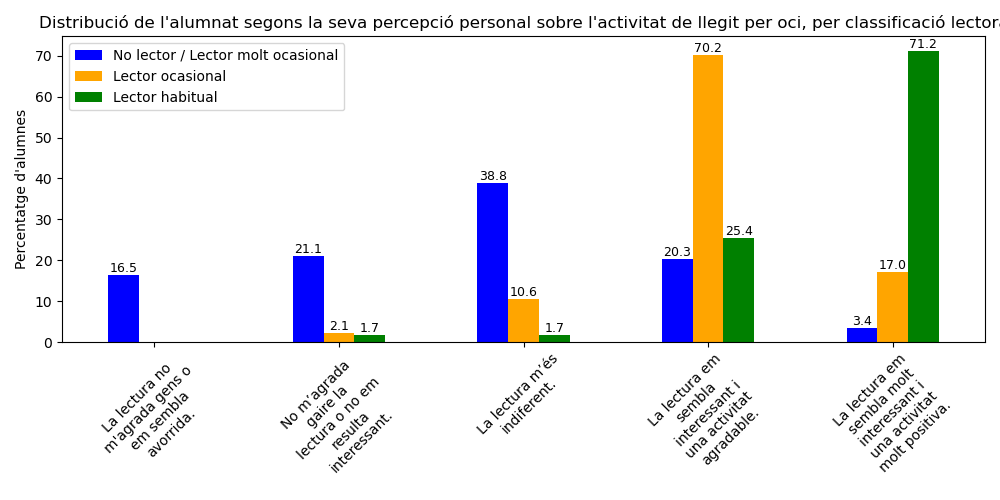
\includegraphics[width=\textwidth]{pictures/9_narrativa_personal_class.png}
    \caption{Distribució de l'alumnat segons la percepció personal sobre la lectura, per classificació lectora.}
    \label{fig:narrativa_personal_class}
\end{figure}

En canvi, la percepció social sobre la lectura no mostra cap associació amb els hàbits lectors per oci (percepció social sobre la lectura vs. temps de lectura: $p = .514$; percepció social respecte a la lectura vs. nombre de llibres: $p = .928$).

Descriptivament, s’observa a la \autoref{fig:narrativa_social} que la major part de l’alumnat considera que, socialment entre els seus iguals, la lectura és vista com una activitat neutra (51.0\%) o poc interessant o avorrida (43.1\%), mentre que només una petita proporció (5.8\%) percep que la lectura és considerada una activitat positiva entre els adolescents. 

\begin{figure}[H]
    \centering
    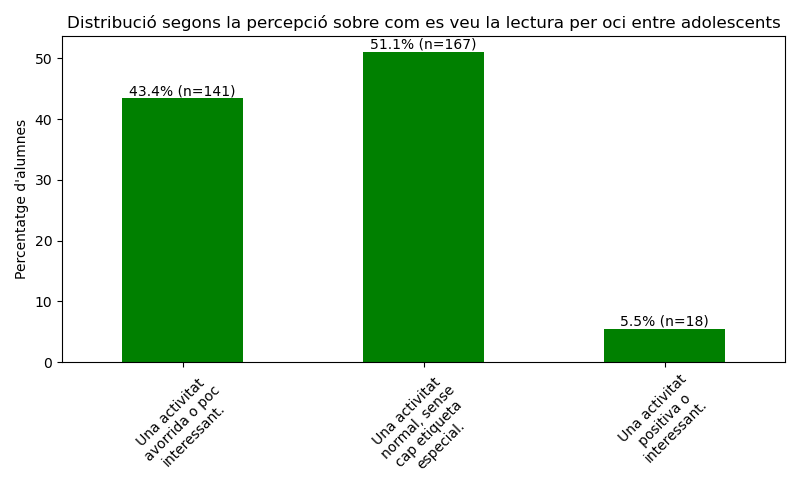
\includegraphics[width=0.85\textwidth]{pictures/9_narrativa_social.png}
    \caption{Distribució de l'alumnat segons la percepció de com es veu socialment la lectura entre els adolescents.}
    \label{fig:narrativa_social}
\end{figure}

Finalment, la freqüència amb què l’alumnat comparteix opinions sobre lectures presenta una associació moderada-forta positiva amb els hàbits lectors, tant amb temps mitjà de lectura setmanal ($\rho = .533$, $p < .001$) com amb el nombre de llibres llegits anualment ($\rho = .552$, $p < .001$).

Descriptivament, s'observa a la \autoref{fig:narrativa_compartir_class} com un 74.2\% dels alumnes no lectors o lectors molt ocasionals no comparteixen mai o quasi mai opinions sobre lectures, respecte al 36.1\% dels lectors ocasionals i al 23.7\% dels lectors habituals, que a més, aquests últims no tenen representació a la categoria ``Mai''. D’altra banda, només un 6.3\% dels no lectors o lectors molt ocasionals comparteixen opinions sobre lectures sovint o molt sovint, respecte al 17.0\% dels lectors ocasionals i al 49.2\% dels lectors habituals.

\begin{figure}[H]
    \centering
    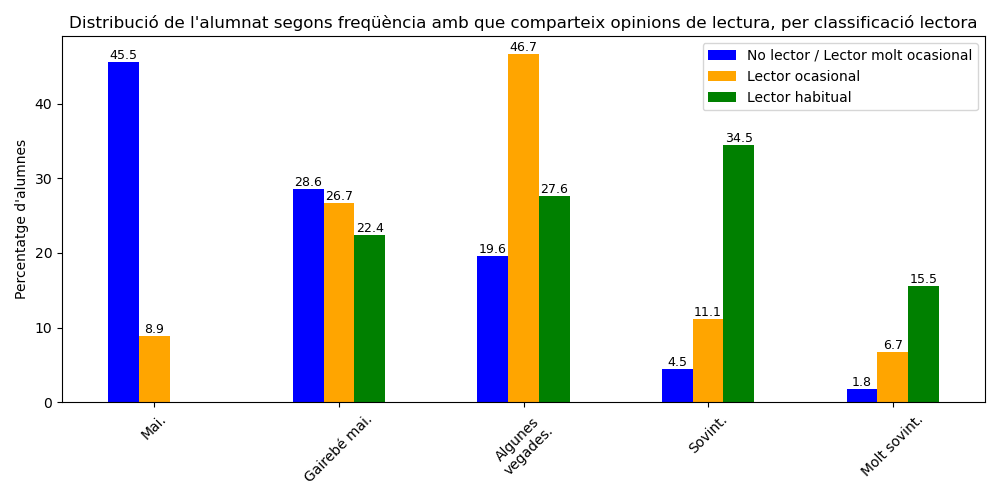
\includegraphics[width=\textwidth]{pictures/9_narrativa_compartir_class.png}
    \caption{Distribució de l'alumnat segons la freqüència amb què comparteixen opinions sobre lectures, per classificació lectora.}
    \label{fig:narrativa_compartir_class}
\end{figure}

\subsection{Lectura per oci, noves tecnologies i xarxes socials}
% ---------------------------------------------------
Pel que fa a la relació entre els hàbits lectors i el temps d’ús de les noves tecnologies, no s’observen associacions estadísticament significatives entre el temps diari dedicat a l’ús de dispositius digitals per a l’oci i els indicadors d’activitat lectora, tant pel que fa al temps de lectura setmanal per oci ($p = .272$), com al nombre de llibres llegits anualment per oci ($p = .805$).

Així mateix, no s'ha trobat cap correlació significativa entre els hàbits lectors i el temps diari mitjà dedicat a veure o sentir contingut audiovisual com sèries, pel·lícules o \emph{streamings} (vs. temps mitjà de lectura setmanal per oci: $p = .600$; vs. nombre de llibres anuals per oci: $p = .759$). D'igual manera, tampoc s'ha trobat cap correlació significativa entre el temps diari mitjà dedicat a jugar a videojocs i el temps mitjà de lectura setmanal per oci ($p = .659$), o el nombre de llibres anuals llegits per oci ($p = .378$).

D'altra banda, s’observen correlacions negatives febles tant amb el temps de lectura setmanal per oci ($\rho = -.163$, $p = .011$) com amb el nombre de llibres llegits anualment ($\rho = -.159$, $p = .013$). Els resultats descriptius (\autoref{fig:tric_time_class}) suggereixen que aquesta correlació feble podria estar relacionada amb una major presència d’alumnat que no llegeix o que llegeix molt ocasionalment entre els qui dediquen més de 3 hores diàries a l’ús de xarxes socials o plataformes de contingut audiovisual ràpid (34.2\%), en comparació amb els lectors ocasionals (25.5\%) i els lectors habituals (13.6\%).

\begin{figure}[H]
    \centering
    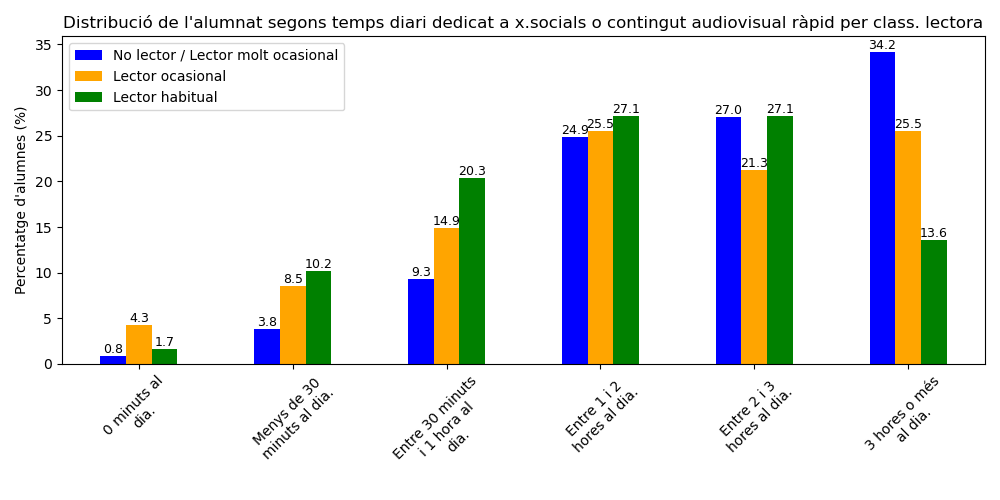
\includegraphics[width=\textwidth]{pictures/10_tric_time_class.png}
    \caption{Distribució de l'alumnat segons el temps diari dedicat a l'ús de xarxes socials o plataformes de contingut audiovisual ràpid, per classificació lectora.}
    \label{fig:tric_time_class}
\end{figure}

Finalment, s'ha estudiat la relació entre el consum de contingut audiovisual relacionat amb la lectura i els hàbits lectors per oci. En aquest sentit, s'han obtingut correlacions positives febles-moderades entre aquesta activitat i el temps de lectura setmanal per oci ($\rho = .319$, $p < .001$), i el nombre de llibres llegits anualment per oci ($\rho = .347$, $p < .001$).

Descriptivament (\autoref{fig:tric_lite_class}) s'observa com un 52.3\% dels no lectors o lectors molt ocasionals afirmen no consumir mai contingut audiovisual relacionat amb la lectura, respecte al 31.9\% dels lectors ocasionals i al 25.4\% dels lectors habituals. En canvi, només un 9.3\% dels no lectors o lectors molt ocasionals consumeix sovint o molt sovint aquest tipus de contingut, proporció que augmenta fins al 23.4\% en els lectors ocasionals i fins al 37.2\% en els lectors habituals.

\begin{figure}[H]
    \centering
    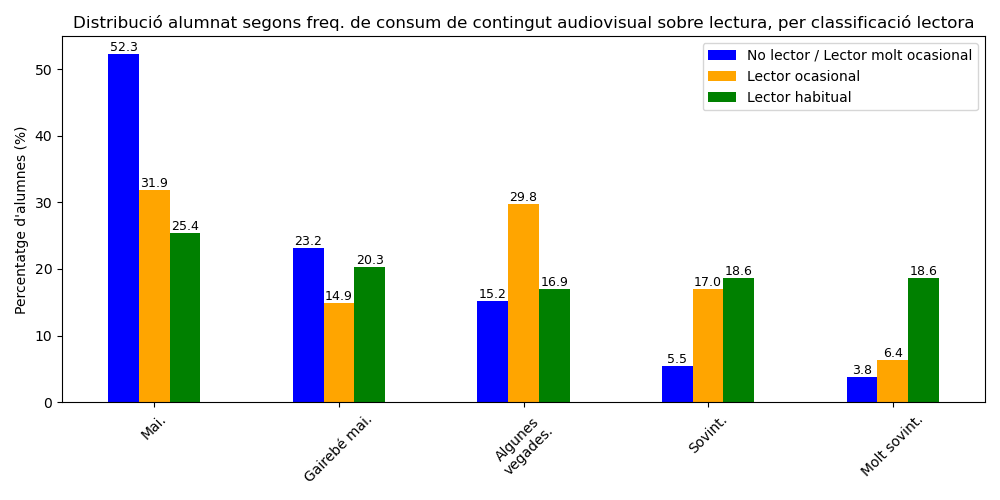
\includegraphics[width=\textwidth]{pictures/10_tric_lite_class.png}
    \caption{Distribució de l'alumnat segons la freqüència amb què consumeixen contingut audiovisual relacionat amb la lectura, per classificació lectora.}
    \label{fig:tric_lite_class}
\end{figure}

Les representacions gràfiques complementàries d’aquests resultats es poden consultar a \autoref{graf:tec}.

\subsection{Lectura per oci i altres activitats d'oci}
% ---------------------------------------------------
Pel que fa a la relació entre els hàbits lectors i altres activitats quotidianes dels estudiants, els resultats mostren patrons diferenciats segons el tipus d’activitat analitzada.

En primer lloc, no s’observa cap associació significativa entre el temps mitjà dedicat a l’estudi i tasques acadèmiques fora de l'horari escolar i els indicadors d’activitat lectora, tant pel que fa al temps mitjà de lectura setmanal ($p = .802$) com al nombre de llibres llegits anualment ($p = .802$). 

Aquest fet contrasta frontalment amb l'opinió de l'alumnat, ja que tal com s'observa a la \autoref{fig:altres_perc}, el 35\% de l’alumnat està molt d'acord amb l'afirmació ``llegiria més llibres o còmics si tingués menys càrrega acadèmica fora d'horari escolar (Exàmens, deures, treballs, etc.)''; i el 20.4\% bastant d'acord. 

\begin{figure}[H]
    \centering
    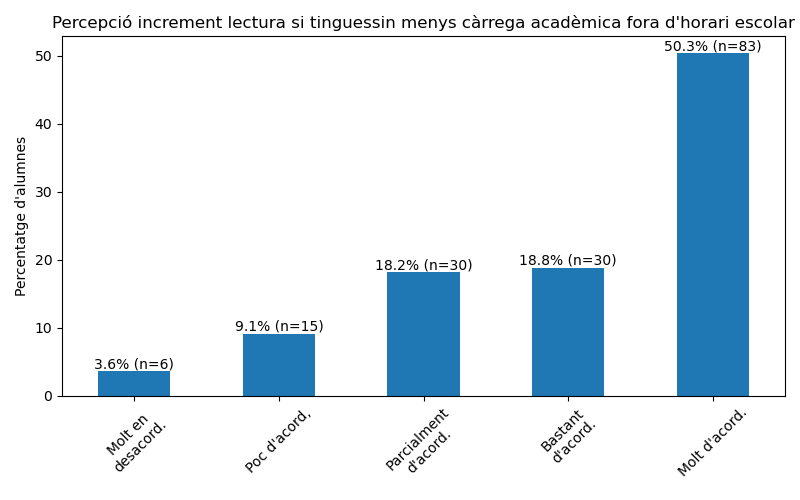
\includegraphics[width=0.85\textwidth]{pictures/11_altres_perc.png}
    \caption{Distribució de l'alumnat segons la percepció que llegirien més per oci si tinguessin menys càrrega acadèmica fora de l'horari escolar.}
    \label{fig:altres_perc}
\end{figure}

De manera similar, tampoc es detecta cap correlació significativa entre la pràctica d’esport i els hàbits lectors per oci (esport vs. temps mitjà setmanal de lectura per oci: $p = .439$; esport vs. nombre de llibres llegits anualment: $p = .443$).

D'altra banda, el temps mitjà dedicat a activitats culturals sí que presenta correlacions positives febles amb el temps de lectura setmanal ($\rho = .247$, $p < .001$) i amb el nombre de llibres llegits anualment ($\rho = .223$, $p < .001$).

L'anàlisi descriptiva (\autoref{fig:altres_cultura_class}) ens mostra que un 57\% dels no lectors o lectors molt ocasionals no dedica, de mitjana, temps setmanal a activitats culturals, envers el 38.3\% dels lectors ocasionals i el 28.8\% dels lectors habituals. En canvi, un 16.9\% dels no lectors o lectors molt ocasionals dedica 1 hora o més al dia a la realització d'activitats culturals, proporció que augmenta fins al 21.2\% en els lectors ocasionals i fins al 32.2\% en els lectors habituals.

\begin{figure}[H]
    \centering
    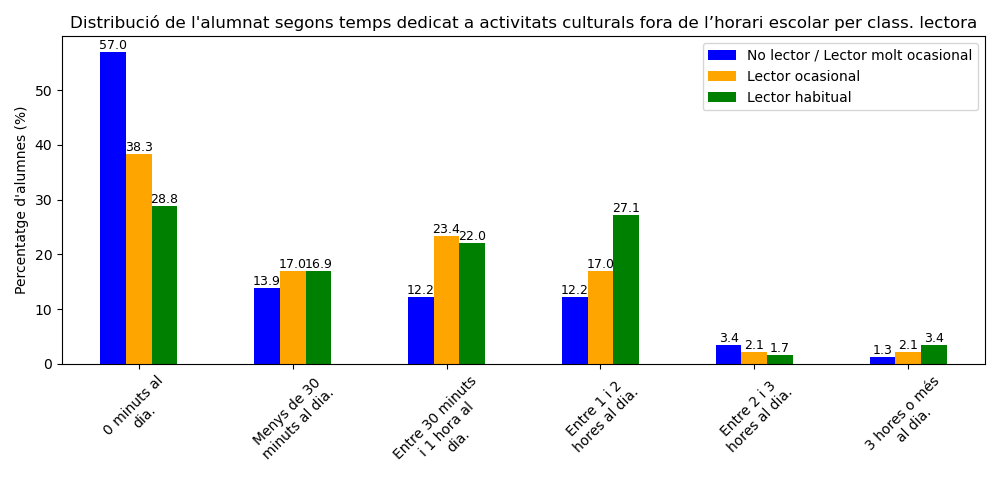
\includegraphics[width=\textwidth]{pictures/11_altres_cultura_class.png}
    \caption{Distribució de l'alumnat segons la freqüència amb què participen en activitats culturals, per classificació lectora.}
    \label{fig:altres_cultura_class}
\end{figure}

Finalment, s'observa que el temps mitjà dedicat a quedar amb amics, amigues o parella sentimental mostra correlacions negatives febles amb el temps mitjà de lectura setmanal ($\rho = -.205$, $p < .001$) i amb el nombre de llibres llegits anualment ($\rho = -.226$, $p < .001$).

Descriptivament, observem a la \autoref{fig:altres_hang_class} que un 24.9\% dels no lectors o lectors molt ocasionals dedica, de mitjana, menys de 30 minuts diaris a quedar amb amics, amigues o parella sentimental, respecte al 42.5\% dels lectors ocasionals i al 49.1\% dels lectors habituals.

\begin{figure}[H]
    \centering
    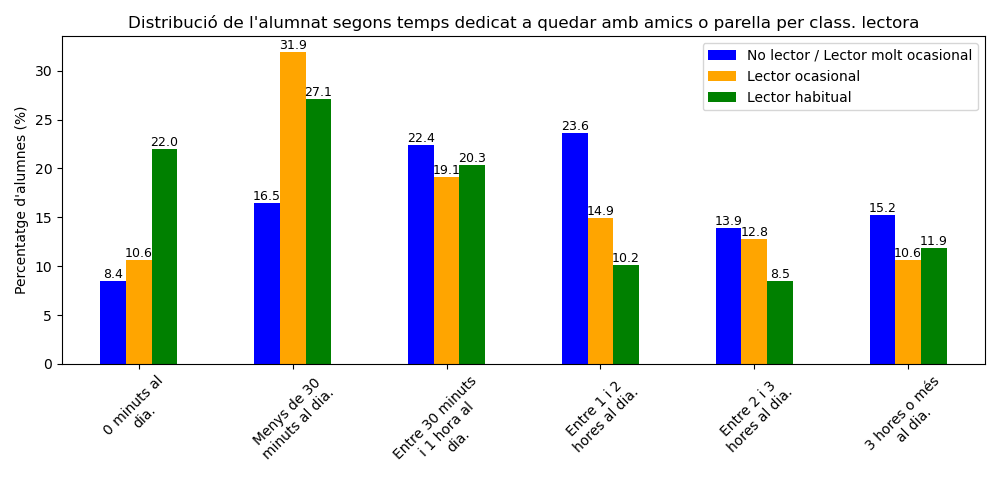
\includegraphics[width=\textwidth]{pictures/11_altres_hang_class.png}
    \caption{Distribució de l'alumnat segons la freqüència amb què surten amb amics, amigues o parella sentimental, per classificació lectora.}
    \label{fig:altres_hang_class}
\end{figure}

\subsection{Lectura per oci i entorn familiar pro-lector}
% ---------------------------------------------------
Pel que fa a l’entorn familiar pro-lector, ni el nivell d'estudis familiars ni la freqüència de veure els pares llegint presenten correlacions estadísticament significatives amb el temps mitjà setmanal dedicat a la lectura ni amb el nombre de llibres llegits anualment. De la mateixa manera, la freqüència de sessions de lectura conjunta amb els pares o tutors legals durant la infància tampoc mostra relacions significatives amb els indicadors de lectura per oci. 

D'altra banda, sí que s’observen correlacions positives febles però estadísticament significatives entre la freqüència de parlar amb les famílies sobre lectures, i, tant el temps de lectura setmanal ($\rho = .261$, $p < .001$) com el nombre de llibres llegits anualment ($\rho = .238$, $p < .001$). 

Descriptivament (\autoref{fig:familia_compartir}) s'observa com un 18.1\% dels no lectors o lectors molt ocasionals no comparteixen mai opinions sobre lectures amb les famílies, respecte al 12.8\% dels lectors ocasionals i al 6.8\% dels lectors habituals. D'altra banda, el 12.3\% dels no lectors o lectors molt ocasionals comparteixen opinions sobre lectures sovint o molt sovint amb les famílies, augmentant fins al 27.7\% en els lectors ocasionals i fins al 45.7\% en els lectors habituals.

\begin{figure}[H]
    \centering
    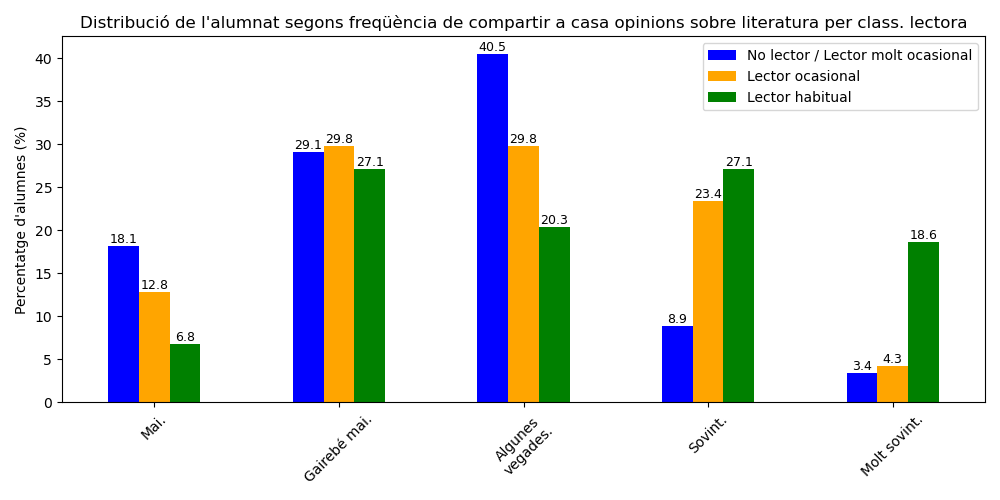
\includegraphics[width=\textwidth]{pictures/12_familia_compartir.png}
    \caption{Distribució de l'alumnat segons la freqüència amb què comparteixen opinions sobre lectures amb les famílies, per classificació lectora.}
    \label{fig:familia_compartir}
\end{figure}

Respecte a la presència de normes clares a casa sobre l'ús de pantalles, els resultats mostren que aquesta variable presenta una correlació positiva molt feble amb el temps de lectura setmanal per oci ($\rho = .195$, $p < .001$) i amb el nombre de llibres llegits anualment per oci ($\rho = .137$, $p = .011$).

Aquest fet s'observa també en l'anàlisi descriptiva (\autoref{fig:familia_normes_class}), on un 51.0\% dels no lectors o lectors molt ocasionals estan en desacord o molt en desacord amb l'afirmació de si tenen normes clares a casa sobre l'ús de pantalles, respecte al 48.9\% dels lectors ocasionals i al 30.5\% dels lectors habituals. D'altra banda, un 20.7\% dels no lectors o lectors molt ocasionals estan d'acord o molt d'acord amb aquesta afirmació, proporció que augmenta fins al 25.5\% en els lectors ocasionals i fins al 44.0\% en els lectors habituals.

\begin{figure}[H]
    \centering
    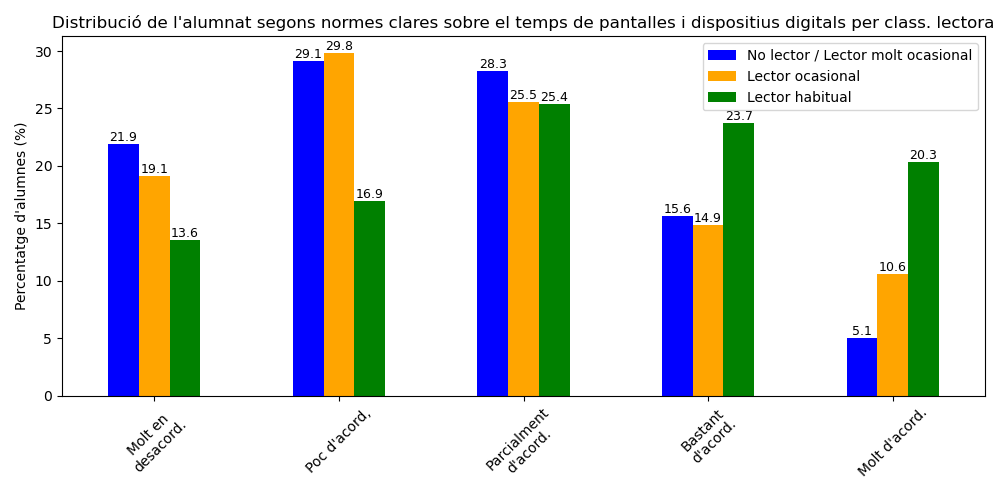
\includegraphics[width=\textwidth]{pictures/12_familia_normes.png}
    \caption{Distribució de l'alumnat segons el grau d'acord amb l'afirmació de si tenen normes clares a casa sobre l'ús de pantalles, per classificació lectora.}
    \label{fig:familia_normes_class}
\end{figure}

Finalment, el nombre de llibres que han tingut disponibles a casa durant la infància i l'adolescència mostra també una relació positiva amb els hàbits lectors per oci (\autoref{fig:familia_llibres}). Un 42.6\% dels no lectors o lectors molt ocasionals declaren haver tingut menys de 26 llibres a la llar, envers el 21.3\% dels lectors ocasionals i al 8.5\% dels lectors habituals. En canvi, un 11.0\% dels no lectors o lectors molt ocasionals afirmen haver tingut més de 200 llibres a la llar durant la seva infància i adolescència, xifra que s'incrementa fins al 10.6\% en els lectors ocasionals i assoleix el 28.8\% en els lectors habituals.

Les correlacions observades respecte d'aquesta qüestió són positives febles, tant amb el temps de lectura setmanal ($\rho = .295$, $p < .001$) com amb el nombre de llibres llegits anualment ($\rho = .300$, $p < .001$).

\begin{figure}[H]
    \centering
    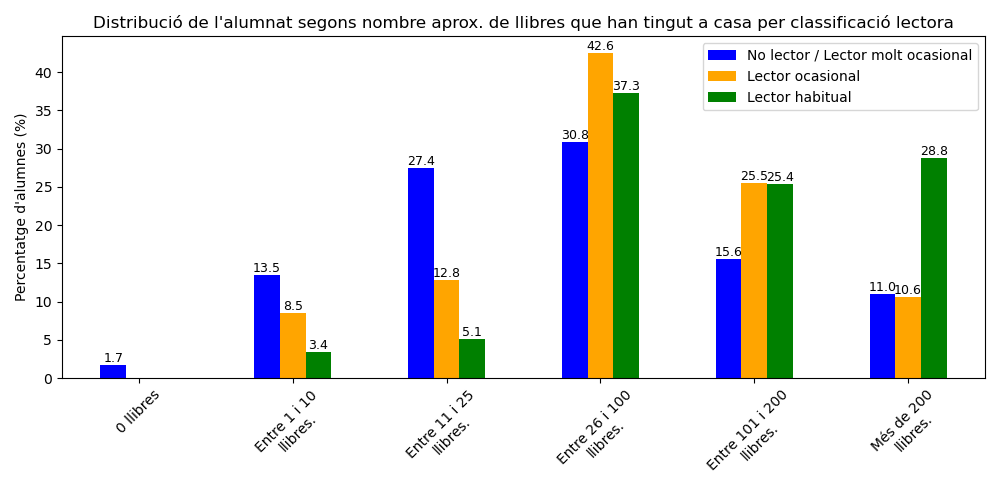
\includegraphics[width=\textwidth]{pictures/12_familia_llibres.png}
    \caption{Distribució de l'alumnat segons el nombre de llibres disponibles a casa durant la infància i l'adolescència, per classificació lectora.}
    \label{fig:familia_llibres}
\end{figure}

\newpage
\subsection{Heatmap de correlacions entre les variables indicadores d'hàbits lectors per oci i la resta de variables analitzades}
% ---------------------------------------------------
\begin{figure}[H]
    \centering
    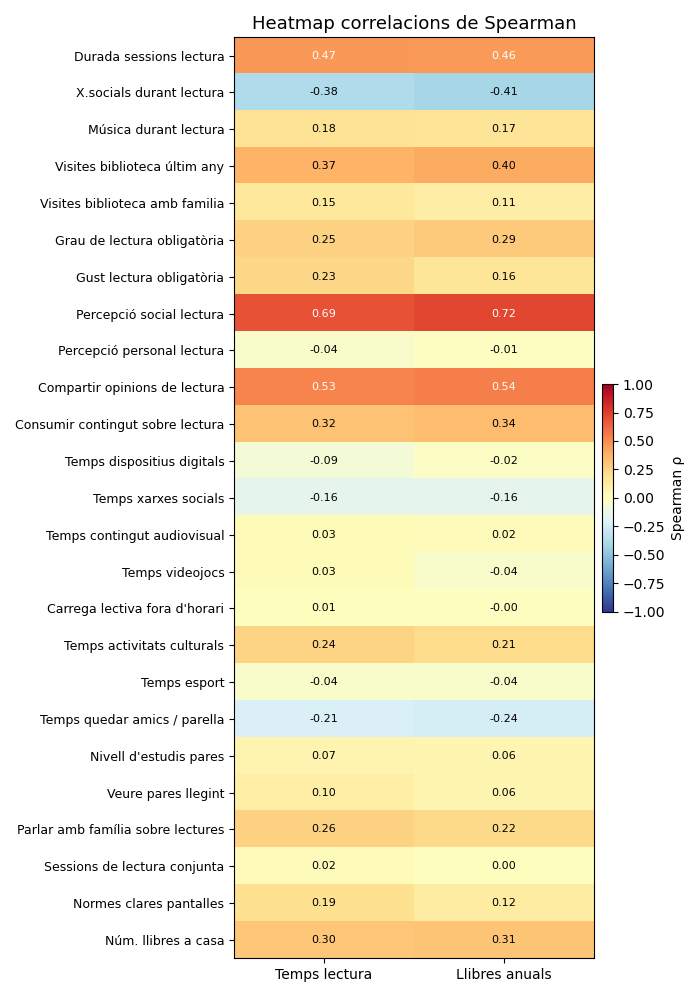
\includegraphics[width=0.9\textwidth]{pictures/13_heatmap.png}
    \caption{\emph{Heatmap} de correlacions entre les variables indicadores d'hàbits lectors per oci i la resta de variables analitzades.}
    \label{fig:heatmap_correlacions}
\end{figure}

\newpage
\section{Discussió dels resultats}
% =======================================================================

% En sintonia, els resultats mostren correlacions negatives moderades de la consulta de xarxes socials durant la lectura amb el temps mitjà de lectura setmanal per oci ($\rho = -.385$, $p < .001$), i també amb el nombre de llibres llegits anualment per oci ($\rho = -.416$, $p < .001$). Aquests resultats suggereixen que una freqüència més elevada de consulta de xarxes socials durant l'activitat lectora s’associa amb nivells més baixos d'hàbits lectors per oci.

% De manera coherent, també s’observa una correlació negativa feble entre la freqüència de consulta de xarxes socials i la durada de les sessions de lectura ($\rho = -.312$, $p < .001$), fet que apunta que una major interrupció de la lectura per l’ús de xarxes socials s’associa amb sessions lectores més curtes.

% Aquest resultat suggereix que la relació observada inicialment podria estar considerablement influenciada per la interpretació contextual de l’ítem dins del qüestionari. En aquest sentit, alguns alumnes van interpretar la pregunta sobre la freqüència d'escoltar música, vídeos o pòdcasts durant la lectura en relació exclusiva amb la lectura per oci, de manera que l’alumnat que no acostuma a llegir per oci ha respost ``mai'' de forma sistemàtica. Això probablement ha contribuït a generar una associació fictícia entre ambdues variables, que es reflecteix en les correlacions febles exposades.

% En relació amb les visites a la biblioteca per agafar llibres o còmics en préstec durant l’últim any (\autoref{fig:tipologia_biblio}), els resultats mostren una baixa freqüència general d’aquesta activitat per part de l’alumnat. En concret,

% Heterogeneitat lectures de l'escola

% Aquests resultats suggereixen que l’alumnat amb hàbits lectors més consolidats tendeix també a llegir en major grau les lectures obligatòries del centre.

%  Aquest fet posa de manifest que, tot i que cap d'ells és un factor clarament determinant, el gust per les lectures obligatòries es relaciona més positivament amb la lectura de les mateixes que el fet de tenir hàbits lectors consolidats per oci.

% Això manifesta que l’alumnat que percep la lectura com una activitat més positiva o interessant tendeix a presentar hàbits lectors per oci més consolidats.

% Aquestes dades contrasten sorprenentment amb la percepció personal sobre la lectura, que és majoritàriament positiva: a la major part de l'alumnat li agrada la lectura, considerant-la una activitat interessant, molt interessant, agradable o molt positiva (44.9\%); mentre que només a un 26.6\% no li agrada la lectura o la percep com una activitat poc interessant o avorrida.

% Podem concloure, per tant, que la percepció personal sobre la lectura presenta una associació positiva i significativa amb els hàbits lectors per oci, de manera que una valoració personal favorable de la lectura s’associa amb uns hàbits lectors més consolidats. En canvi, la percepció social de la lectura no mostra cap relació significativa amb els hàbits de lectura per oci, fet que posa de manifest que la valoració social percebuda entre iguals no constitueix un factor determinant per a l'establiment d'hàbits lectors per oci consolidats.

% Aquest resultat suggereix que els estudiants que participen més en interaccions socials relacionades amb la lectura tendeixen a presentar majors hàbits lectors per oci.

% WIPW: Pel que fa a la relació entre els hàbits lectors i el temps d'ús de les noves tecnologies, els resultats mostren una realitat més complexa que una simple oposició entre lectura i pantalles. En primer lloc, el temps diari mitjà dedicat a l’ús de dispositius digitals per a l’oci ---tot i ser aquest molt més elevat en el conjunt de la mostra que el temps dedicat a la lectura per oci--- no mostra associacions significatives amb els indicadors d’activitat lectora

% Aquests resultats suggereixen que, malgrat la digitalització actual de l’entorn juvenil, l'alumnat de l'escola continua preferint el format físic per a la lectura per oci.

% suggerint que les sessions més llargues tendeixen significativament a associar-se amb un hàbit lector més consistent. 

%  suggerint que una major vinculació amb la biblioteca s’associa amb hàbits lectors per oci més consolidats.

% encara que el temps diari mitjà dedicat a l’ús de xarxes socials o plataformes de contingut audiovisual ràpid és molt més elevat en el conjunt de la mostra (\autoref{fig:tric_time}) que el temps mitjà dedicat a la lectura per oci, la seva relació amb els hàbits lectors per oci és reduïda. 

% Per aquest motiu, tot i existir una lleugera tendència associada a una menor activitat lectora amb un ús més elevat de xarxes socials, no podem afirmar que el temps diari mitjà dedicat a l’ús de xarxes socials actuï com un factor determinant en els hàbits lectors de l’alumnat per oci.

% Aquest patró apunta que, si bé l’ús de xarxes socials no actua necessàriament com un competidor directe de la lectura per oci, un ús intensiu sí que podria associar-se a nivells lleugerament més baixos d’activitat lectora, tot i que la magnitud d’aquesta relació és reduïda.

% TOT I mols lectors habituals no tenir un patró clar de lectura, són els que més... Sembla que hi ha una tendencia de sessions mes llargues, mes habits de lectura.

% suggerint que la narrativa social adolescent de la lectura no està directament vinculada amb els hàbits lectors per oci dels alumnes.

% , assenyalant que un consum més elevat de contingut audiovisual relacionat amb la lectura s’associa de forma moderada amb hàbits lectors més consolidats.

% Aquest fet suggereix que el consum de contingut audiovisual relacionat amb la lectura podria estar actuant com un estimul que reforça els hàbits lectors per oci de l'alumnat del centre.

% Els resultats obtinguts suggereixen que, tot i que la percepció de la càrrega acadèmica com a factor limitant per a la lectura per oci està força generalitzada entre l’alumnat, aquesta no es tradueix en una relació significativa entre el temps dedicat a estudiar o realitzar tasques acadèmiques fora de l'horari escolar i els hàbits lectors per oci.

% Aquests resultats suggereixen que els alumnes que dediquen, de mitjana, més temps setmanal a activitats culturals tendeixen a llegir més habitualment per oci, formant ambdues activitats part d’un mateix perfil ampli d’interessos i preferències d’oci.

% determinant que aquests factors no influeixen de manera significativa en els hàbits lectors per oci de l’alumnat

% Aquests resultats suggereixen que parlar habitualment amb les famílies sobre lectura s'associa positivament amb hàbits lectors per oci més consolidats, i són coherents amb els resultats obtinguts a l’apartat \nameref{sec:narrativa}, on també es va observar una relació positiva entre el fet de compartir opinions sobre lectures amb amistats i els hàbits lectors per oci.

% Tanmateix, compartir opinions amb amics i amigues presenta una associació més forta amb els hàbits lectors que compartir opinions amb les famílies, suggerint que les interaccions socials entre iguals al voltant de la lectura podrien tenir un paper més rellevant en la consolidació dels hàbits lectors per oci que les interaccions familiars.

% , suggerint que la presència de normes clares a casa sobre l'ús de pantalles podria estar lleugerament associada amb hàbits lectors per oci més consolidats, tot i que la magnitud d’aquesta relació és reduïda. 

%  reforçant la idea que disposar d’un entorn familiar amb més accés a llibres durant el desenvolupament podria afavorir, parcialment, el desenvolupament d’hàbits lectors.

\subsection{Hàbits lectors per oci baixos en el conjunt de la mostra}
% ---------------------------------------------------
Els resultats obtinguts mostren que els hàbits lectors de llibres o còmics per oci de l'alumnat del centre són baixos en termes generals. La major part de la mostra es concentra en les categories de 0 o menys de 30 minuts de temps mitjà dedicat a la setmana a la lectura de llibres o còmics per oci (67.9\%, $n = 233$), i de cap o 1-2 llibres o còmics llegits anualment per oci (61.2\%, $n = 210$ ). Una dada reveladora és que més de la meitat de l'alumnat (51.3\%, $n = 176$) dedica 0 minuts, de mitjana en una setmana habitual, a la lectura de llibres o còmics per oci.

De manera coherent, el nombre de pàgines estimades llegides per oci de llibres o còmics durant l'últim any és, en general, també molt baix; amb una mitjana de 1191 pàgines i una mediana de 300 pàgines. Aquests estadístics tan baixos i la gran diferència entre mitjana i mediana ens indiquen una asimetria positiva en la distribució: la major part de l'alumnat ha llegit molt poques pàgines estimades de llibres o còmics per oci aquest últim any, mentre que una minoria de lectors habituals n'ha llegit una quantitat considerable, elevant així la mitjana i la desviació típica de la distribució.

En consonància, la classificació lectora construïda a partir dels indicadors de temps mitjà setmanal de lectura de llibres o còmics per oci, i del nombre de llibres o còmics llegits l'últim any per oci, situa la majoria dels participants (69.1\%, $n = 236$) en la categoria de \emph{no lector / lector molt ocasional}.

// WIP: Relacionar con literatura existente

// WIP: Relacionar con las entrevistas semiestructuradas

Tal com s'ha esmentat, malgrat la baixa freqüència general de lectura de llibres o còmics per oci, també s’observa l’existència d’un grup reduït però clarament consolidat de lectors habituals, amb volums de lectura molt superiors a la resta de la mostra. Aquest fet, com hem vist, és el que provoca una que la distribució sigui fortament asimètrica, suggerint una elevada polarització dels hàbits lectors de llibres o còmics per oci dins l’alumnat.

\subsection{Diferències de gènere en els hàbits lectors per oci}
% ---------------------------------------------------
Quant al gènere, les noies presenten nivells de lectura de llibres o còmics per oci clarament superiors als dels nois en pràcticament tots els indicadors analitzats: temps mitjà de lectura setmanal (\autoref{fig:temps_genere}), nombre de llibres o còmics llegits l'últim any (\autoref{fig:llibres_genere}), volum estimat de pàgines llegides l'últim any (\autoref{fig:pagines_boxplot_genere}) i classificació lectora (\autoref{fig:classificacio_genere}).

Tanmateix, els resultats també mostren que existeix heterogeneïtat dins dels dos grups. Tot i la menor activitat lectora general dels nois, també n'hi ha amb hàbits lectors per oci consolidats, de la mateixa manera que una part considerable de les noies presenta nivells baixos de lectura habitual per oci. Aquest fet s'observa clarament en el \emph{boxplot} de la \autoref{fig:pagines_boxplot_genere} i a la \autoref{tab:estadistics_pagines_genere}.

En consonància, els marcadors estadístics utilitzats per mesurar la influència del gènere en els hàbits lectors indiquen que, tot i existir diferències estadísticament significatives entre nois i noies, la magnitud d’aquestes associacions és baixa. Això suggereix que el gènere es relaciona amb els hàbits lectors per oci, però que existeixen altres factors amb un paper més rellevant en la configuració dels hàbits lectors de l’alumnat.  

Per concloure aquest apartat, cal destacar les diferències observades en les preferències temàtiques de lectura per oci segons el gènere. Les noies mostren una preferència especialment marcada per la novel·la romàntica i la novel·la fantàstica, mentre que els nois la mostren principalment pels còmics i, en grau més baix, també per la novel·la fantàstica.

\subsection{Diferències en els hàbits lectors per oci en funció del curs i l'itinerari del batxillerat}
% ---------------------------------------------------
Quant al curs acadèmic i a l’itinerari de batxillerat, no s’observen diferències clares ni consistents en els hàbits de lectura per oci. En el cas del curs, no es detecta una tendència evolutiva entre nivells educatius que permeti afirmar que els hàbits lectors augmentin o disminueixin de manera consistent a mesura que l’alumnat avança en l’etapa educativa; tot i que 4t d'ESO destaca especialment per presentar indicadors de lectura més baixos que la resta de cursos. 

De la mateixa manera, l'itinerari del batxillerat ---Ciències Socials o Ciències i Tecnologia--- no sembla exercir una influència destacable sobre els hàbits lectors per oci de l’alumnat del centre.

\subsection{Lectura per oci i lectures obligatòries de l'escola}
% ---------------------------------------------------
Els resultats obtinguts mostren que la relació entre el grau de lectura de les lectures obligatòries del centre i els hàbits lectors de llibres o còmics per oci és limitada. Tot i que s’observa una tendència a un major compliment de les lectures obligatòries entre l’alumnat amb hàbits lectors més consolidats, les correlacions són febles, la qual cosa suggereix que la lectura acadèmica i la lectura per oci no constitueixen dimensions fortament associades.

En general, la valoració de les lectures obligatòries és considerablement negativa, ja que només un 9.9\% ($n = 34$) de l’alumnat declara que li agraden bastant o molt. Tanmateix, una part significativa de l’alumnat indica que llegiria més aquestes lectures si s’ajustessin millor als seus interessos personals. En aquest sentit, els resultats estadístics mostren una relació moderada entre el gust per les lectures obligatòries i el grau en què aquestes es llegeixen; suggerint que, en aquest cas, potser tenen raó. 

En conjunt, els resultats apunten a una certa desconnexió entre les preferències lectores de l’alumnat i les lectures proposades en l’àmbit escolar, fet que podria incidir en el nivell de lectura d’aquestes. D’aquesta manera, les lectures obligatòries del centre, almenys tal com són percebudes per una part rellevant de l’alumnat, no actuen com un factor clar de promoció dels hàbits lectors per oci.

\subsection{Lectura per oci, una activitat social}
% ---------------------------------------------------
Un dels resultats més rellevants de la investigació és la importància de la percepció personal sobre la lectura i les interaccions socials al voltant d'aquesta en la configuració dels hàbits lectors per oci de l'alumnat del centre. En aquest sentit, els resultats mostren que tenir una percepció personal positiva sobre la lectura s'associa amb hàbits lectors per oci més consolidats.

D'altra banda, la percepció social sobre la lectura entre els adolescents no mostra una associació significativa amb els hàbits lectors per oci, suggerint que aquesta variable no té rellevància en els hàbits lectors de l’alumnat del centre. Descriptivament, la major part de l’alumnat considera que la lectura és socialment percebuda com una activitat neutra o negativa, mentre que només una proporció reduïda considera que es percep socialment com a positiva. Aquest fet contrasta fortament amb la percepció personal sobre la lectura, que és majoritàriament positiva entre l’alumnat. 

Pel que fa a la interacció social al voltant de la lectura, els alumnes que comparteixen més sovint opinions sobre lectures amb amistats o entorns propers també presenten hàbits lectors més consolidats. Això reforça la idea que la lectura no és exclusivament una activitat individual, sinó que funciona com una pràctica social vinculada a la interacció, la recomanació, l’intercanvi d’experiències lectores i el sentit de pertinença a un grup lector.

De manera coherent, els resultats relacionats amb el consum de contingut audiovisual sobre llibres o lectura també apunten en aquesta direcció. Lluny d’actuar com a competidor de la lectura, dedicar temps a veure o sentir aquest tipus de contingut sembla funcionar com un espai de socialització lectora, on els adolescents poden descobrir nous llibres, compartir recomanacions i sentir-se part d’una comunitat lectora.

\subsection{Lectura per oci, noves tecnologies i xarxes socials}
% ---------------------------------------------------
Els resultats obtinguts qüestionen la idea generalitzada que les noves tecnologies i les xarxes socials afecten directament i de manera significativa als hàbits de lectura de llibres o còmics per oci de l'alumnat. Ni el temps dedicat a dispositius digitals en general, ni el dedicat a veure sèries, pel·lícules, \emph{streamings} o jugar a videojocs mostren relacions significatives amb els hàbits lectors per oci. Aquest fet suggereix que aquestes activitats no actuen com a competidores directes de la lectura per oci, i que, per tant, es descarta que un ús més intensiu de les noves tecnologies impliqui necessàriament una menor activitat lectora de llibres o còmics per oci en l'alumnat del centre.

Tanmateix, sí que s’observa una relació negativa feble entre els hàbits lectors i l’ús intensiu de xarxes socials o plataformes de contingut audiovisual ràpid. Tot i la baixa magnitud de les correlacions, els resultats descriptius mostren una presència més elevada de no lectors entre l’alumnat que dedica moltes hores diàries a aquest tipus de consum digital.

// WIP: Relacionar amb entrevistes semi: J.R. Mont. i amb treball sobre adolescència i xarxes socials que vas fer a psico.

En aquesta línia, els resultats sobre la consulta freqüent de xarxes socials durant la lectura reforcen aquesta interpretació. L’alumnat que interromp més sovint la lectura per consultar xarxes socials tendeix a presentar sessions lectores més curtes i uns hàbits lectors menys consolidats.

Potser per aquest motiu, el format àmpliament preferit per l’alumnat per a la lectura de llibres o còmics per oci continua sent el format físic o en paper tradicional (88.4\%, $n = 205$). Els formats digitals, com els \emph{ebooks}, les plataformes de lectura digital, els audiollibres o els arxius PDF, tenen una presència molt minoritària com a formats preferents per a la lectura de llibres o còmics per oci en la mostra. Aquest resultat suggereix que, malgrat la digitalització creixent de l’entorn juvenil, i la gran quantitat d'hores dedicades a l'ús de tecnologies digitals per a l'oci (\autoref{fig:tec_time}), la lectura per oci continua essent una activitat vinculada principalment al suport físic tradicional per a l'alumnat del centre.

\subsection{Lectura per oci i entorn familiar pro-lector}
% ---------------------------------------------------
L'anàlisi dels resultats obtinguts sobre aquesta qüestió determinen una influència moderada de l'entorn familiar pro-lector en els hàbits lectors de llibres o còmics per oci de l'alumnat del centre. Factors tradicionalment associats a un increment de l'interès per la lectura com el nivell d'estudis familiars, la freqüència de veure els pares llegint o la freqüència amb què s'han realitzat sessions de lectura conjunta amb les famílies durant la infància i adolescència, no presenten relacions estadísticament significatives amb els hàbits lectors per oci dels estudiants. 

D'altra banda, el nombre de llibres disponibles a la llar durant la infància i adolescència i la freqüència de parlar o compartir opinions sobre lectures amb les famílies sí que mostren associacions positives significatives amb els hàbits de lectura de llibres o còmics per oci, encara que de magnitud feble.

Especialment rellevant és la relació observada entre compartir opinions sobre lectures amb la família i els hàbits lectors per oci...

// WIP: Relacionar amb Berger y Arnett. Y un poco con lo que tambien aparece en el apartado social

Un altre aspecte interessant és que la presència de normes clares a casa sobre l’ús de pantalles mostra una relació estadísticament significativa amb els hàbits lectors per oci, però de magnitud molt feble. Tenint en compte aquesta intensitat reduïda, així com el fet que l’ús de xarxes socials encara presenta una associació més feble, aquest resultat sembla indicar que la influència d’aquestes normes podria estar vinculada a altres factors més amplis ---com més implicació familiar en l'educació dels fills i filles---, els quals sí que podrien tenir un efecte lleuger sobre la lectura per oci.

\newpage
\section{Conclusions}
% =======================================================================
L'objectiu d'aquesta recerca era realitzar una anàlisi descriptiva complerta sobre els hàbits de lectura per oci de l'alumnat del centre, així com sobre la relació d'aquests amb diferents factors personals, socials, contextuals i familiars. 

Els resultats obtinguts han permès la consecució d'aquests objectius, construint una fotografia global i exhaustiva dels hàbits de lectura per oci de l'alumnat del centre i dels diferents factors que es troben associats al seu desenvolupament.

En termes generals, s’observa que la lectura de llibres o còmics per oci és una activitat poc freqüent en la major part de l'alumnat, amb una distribució clarament asimètrica. La majoria dels estudiants presenta nivells inexistents o molt baixos de lectura habitual de llibres o còmics per oci, mentre que un grup reduït, però clarament consolidat de lectors habituals presenta nivells de lectura de llibres o còmics molt superiors a la resta de la mostra.

Pel que fa als factors analitzats, el gènere es confirma com una variable significativa associada als hàbits lectors, amb nivells de lectura més elevats en les noies que en els nois. Tanmateix, aquesta relació presenta una magnitud baixa, fet que indica que, tot i la seva significació estadística, el gènere no constitueix per si sol un factor determinant dels hàbits lectors.

En canvi, altres variables tradicionalment considerades rellevants, com el temps dedicat a tecnologies digitals, sèries, pel·lícules, videojocs o plataformes de \emph{streaming}, no mostren una relació significativa amb la lectura per oci. Això suggereix que l’ús de pantalles, en si mateix, no desplaça necessàriament l’activitat lectora.

D'altra banda, el temps dedicat a xarxes socials o a plataformes de contingut audiovisual ràpid mostra una associació negativa feble amb els hàbits lectors per oci, així com el fet de consultar-les amb freqüència durant les sessions de lectura. Aquestes relacions, tot i la seva baixa magnitud i limitada incidència global sobre els hàbits lectors, podrien suggerir que un ús intensiu d’aquest tipus de plataformes s’associa lleugerament amb uns hàbits lectors menys consolidats, o bé amb un perfil d’alumnat que prioritza aquest tipus de consum digital en detriment de la lectura per oci.

Un altre resultat rellevant de la recerca és el paper combinat de la dimensió personal i relacional en els hàbits de lectura per oci de l'alumnat del centre. En aquest sentit, la percepció personal de la lectura com una activitat positiva s’associa de manera significativa amb uns hàbits lectors per oci més consolidats, mentre que la percepció social general de la lectura entre iguals no mostra una relació significativa amb aquests hàbits. En canvi, la interacció social directa al voltant de la lectura ---com ara compartir opinions, recomanacions o contingut audiovisual relacionat--- sí que presenta una associació positiva amb els hàbits lectors per oci, suggerint que la lectura es veu reforçada quan es vincula a processos de reconeixement i pertinença a un grup o comunitat lectora.

// WIP añadir relacion con entrevistas semiestructuradas y Berger o Arnett.

Pel que fa a l’àmbit familiar, els resultats mostren una influència parcial. Mentre que alguns indicadors, com la disponibilitat de llibres a la llar o la comunicació al voltant de la lectura, presenten associacions positives; altres factors tradicionalment considerats rellevants, com el nivell d'estudis dels pares, les visites a la biblioteca durant la infància, veure els pares llegir o realitzar activitats de lectura conjuntes, no mostren relacions significatives amb els hàbits lectors per oci. En conjunt, la influència familiar sobre els hàbits de lectura de llibres i còmics per oci en els alumnes del centre existeix, però és més limitada i indirecta del que sovint es considera.

//WIP: Meter el caso de M.J. con sus hijos, o que quizás en el futuro, tener en cuenta que son adolescentes, etc.

Finalment, els resultats indiquen una relació limitada entre les lectures obligatòries del centre i els hàbits lectors per oci. Tot i que es detecta una tendència a un major compliment de les lectures obligatòries entre l’alumnat amb hàbits lectors més consolidats, aquesta associació és feble, i la valoració general de les lectures obligatòries és negativa. Aquest fet suggereix que les lectures obligatòries no estan actuant com un factor clar de promoció dels hàbits lectors per oci, i que la desconnexió entre les preferències lectores de l’alumnat i les lectures proposades en l’àmbit escolar podria incidir, tant en el grau de compromís amb aquestes, com en els hàbits lectors per oci dels alumnes del centre.

En síntesi, els resultats apunten que els hàbits lectors per oci de l’alumnat del centre s’expliquen a partir d’una combinació de factors personals i socioculturals, amb un pes especialment rellevant de la dimensió perceptiva i de la interacció social directa al voltant de la lectura. En aquest sentit, la percepció personal positiva de la lectura apareix com un dels principals factors associats als hàbits lectors, mentre que la dimensió social no opera a través de la valoració general de la lectura entre iguals, sinó mitjançant la participació en pràctiques compartides, com ara comentar, recomanar o intercanviar experiències lectores, que contribueixen a reforçar una identitat vinculada a la pertinença a un grup o comunitat lectora.

D'altra banda, variables com el gènere, la dedicació de temps setmanal a activitats culturals, el nombre de llibres disponibles a la llar durant la infància, el grau en què es llegeixen les lectures obligatòries del centre, les visites realitzades a biblioteques durant l'últim any per agafar llibres o còmics en préstec i l'ús de xarxes socials o plataformes de contingut audiovisual ràpid, també es relacionen amb els hàbits lectors de l'alumnat de l'institut, però de manera més limitada. 

Els altres factors analitzats no mostren relacions estadísticament significatives amb els hàbits lectors per oci, suggerint que no tenen un paper rellevant en la configuració d'aquests hàbits en els alumnes del centre.

% =======================================================================
\ifstartwithtitle
  \newpage
\fi
\printbibliography

% =======================================================================
\newpage
\appendix

\section{Gràfics i taules complementaries}
% =======================================================================

\subsection{Gràfics complementaris descriptius de la mostra}
\label{graf:descript_mostra}

La distribució per cursos és la següent: el 32.1\% ($n =$ 110) dels alumnes pertany a 3r d'ESO, el 21.6\% ($n =$ 74) dels alumnes són de 4t d'ESO, el 25.1\% ($n =$ 86) dels alumnes cursa 1r de Batxillerat i el 21.3\% ($n =$ 73) dels alumnes està acabant 2n de Batxillerat.   

\begin{figure}[H]
    \centering
    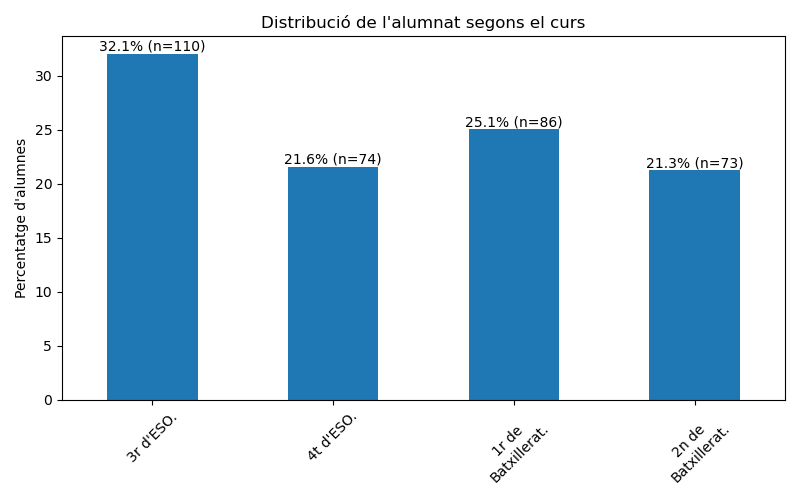
\includegraphics[width=0.85\textwidth]{pictures/1_descriptive_curs.png}
    \caption{Distribució de l'alumnat segons el curs.}
    \label{fig:descriptive_curs}
\end{figure}

Quant a l’itinerari de Batxillerat, el 32.7\% ($n =$ 56) de l’alumnat cursa la modalitat de Ciències Socials, mentre que el 67.3\% ($n =$ 115) cursa la modalitat de Ciències i Tecnologia. El centre no disposa de cap altra modalitat de Batxillerat.

\begin{figure}[H]
    \centering
    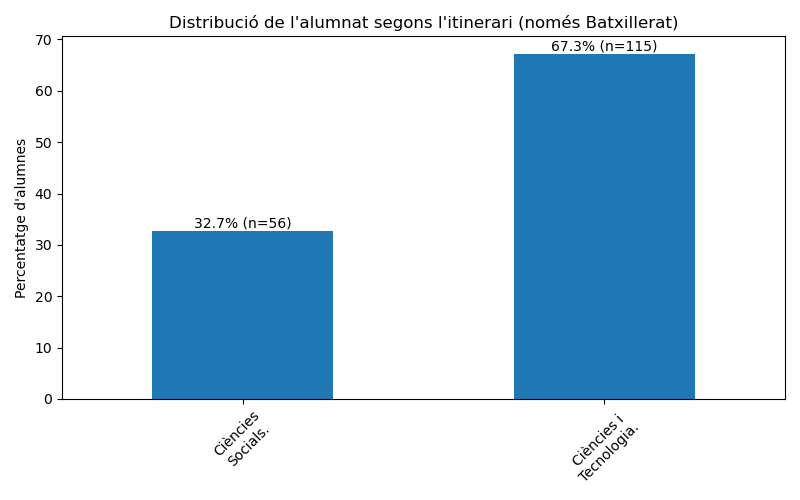
\includegraphics[width=0.85\textwidth]{pictures/1_descriptive_itinerari.png}
    \caption{Distribució de l'alumnat segons la modalitat del Batxillerat.}
    \label{fig:descriptive_itinerari}
\end{figure}

\subsection{Gràfics complementaris de temps mitjà de lectura setmanal i llibres o còmics llegits en els últims 12 mesos per oci}
\label{graf:descript_llibres_temps}

\begin{figure}[H]
    \centering
    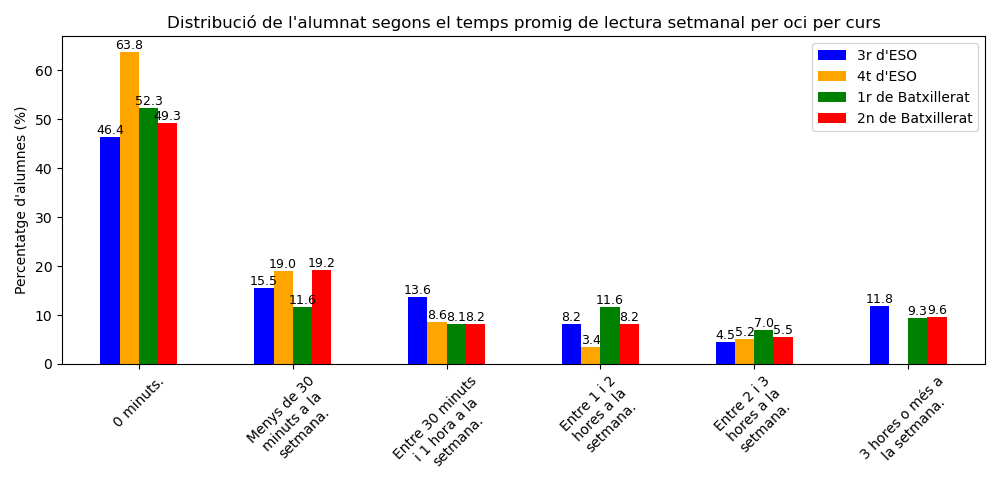
\includegraphics[width=\textwidth]{pictures/2_temps_curs.png}
    \caption{Distribució de l'alumnat segons el temps mitjà setmanal dedicat a la lectura de llibres o còmics per oci per curs.}
    \label{fig:temps_curs}
\end{figure}

\begin{figure}[H]
    \centering
    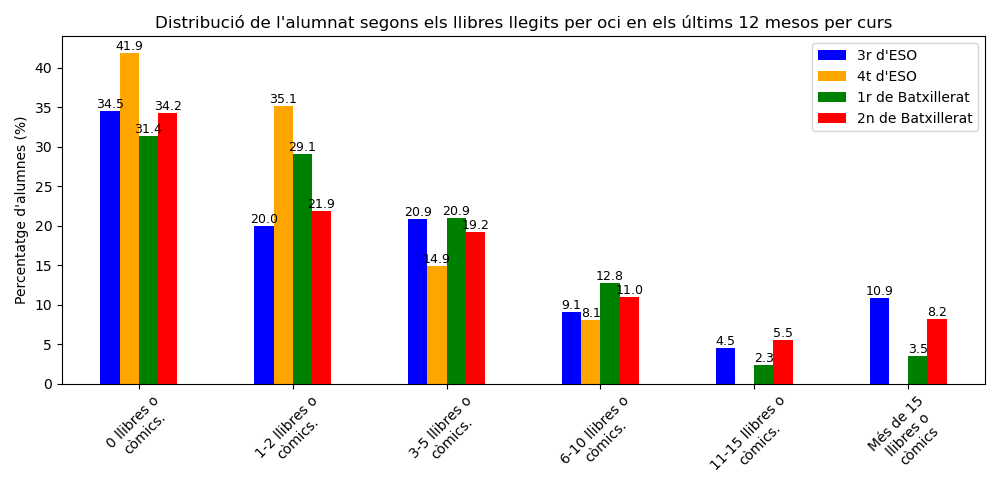
\includegraphics[width=\textwidth]{pictures/2_llibres_curs.png}
    \caption{Distribució de l'alumnat segons el nombre de llibres o còmics llegits en els últims 12 mesos per oci per curs.}
    \label{fig:llibres_curs}
\end{figure}

\begin{figure}[H]
    \centering
    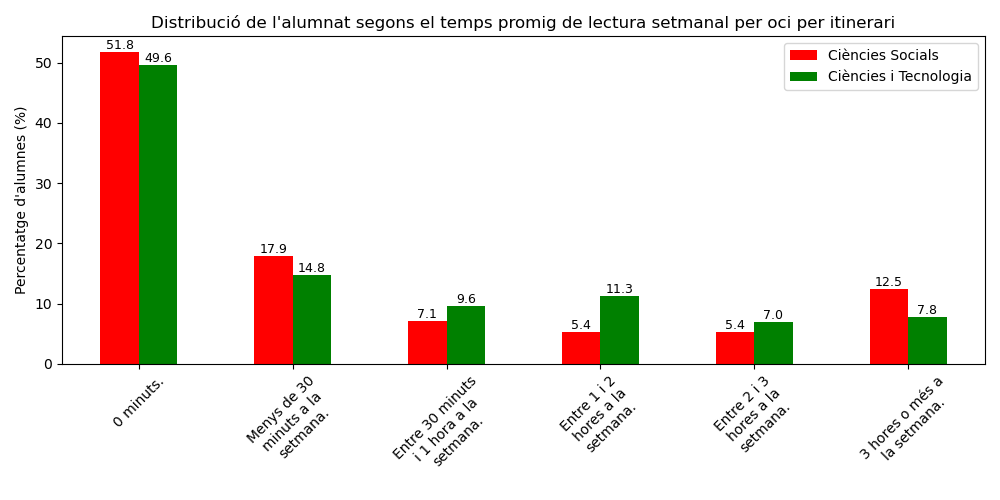
\includegraphics[width=\textwidth]{pictures/2_temps_itinerari.png}
    \caption{Distribució de l'alumnat segons el temps mitjà de lectura setmanal de llibres o còmics per oci per modalitat de Batxillerat.}
    \label{fig:temps_itinerari}
\end{figure}

\begin{figure}[H]
    \centering
    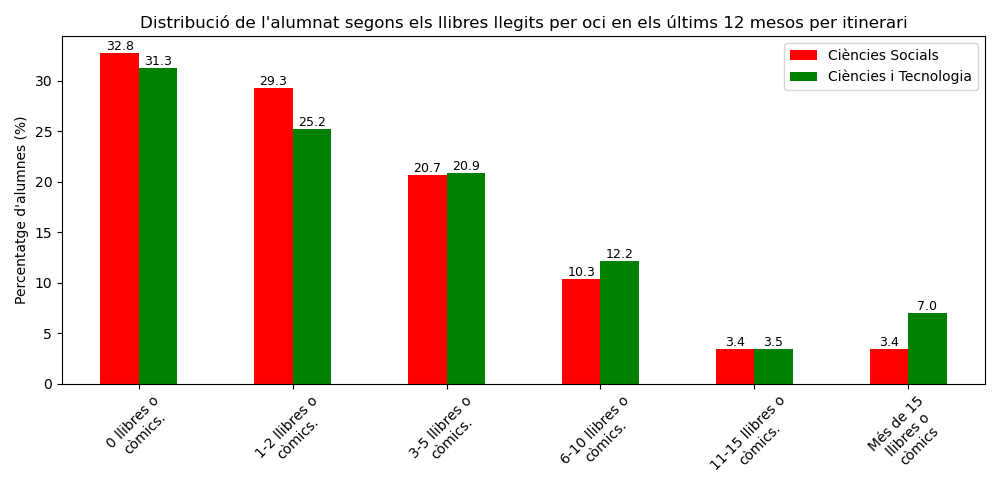
\includegraphics[width=\textwidth]{pictures/2_llibres_itinerari.png}
    \caption{Distribució de l'alumnat segons el nombre de llibres o còmics llegits en els últims 12 mesos per oci per modalitat de Batxillerat.}
    \label{fig:llibres_itinerari}
\end{figure}

\subsection{Taules complementaries nombre de pàgines llegides per oci en els últims 12 mesos}
\label{graf:descript_pag}

\begin{table}[H]
\centering
\begin{tabular}{lrr}
\hline
\textbf{Estadístics} & \textbf{Ciències Socials} & \textbf{Ciències i Tecnologia} \\
\hline
$n$ & 58 & 115 \\
$\bar{x}$ & 1078.45 & 1343.70 \\
$s$ & 1741.25 & 2191.36 \\
$\min(x)$ & 0 & 0 \\
$Q_1$ & 0 & 0 \\
$Q_2$ (mediana) & 300 & 300 \\
$Q_3$ & 1400 & 1600 \\
$\max(x)$ & 8100 & 12600 \\
\hline
\end{tabular}
\vspace{0.5em}
\caption{Estadístics descriptius de la variable pàgines estimades llegides anualment per oci en funció de la modalitat de batxillerat.}
\label{tab:estadistics_pagines_modalitat}
\end{table}

\subsection{Gràfics complementaris de lectura per oci, narrativa adolescent i percepcions personals sobre la lectura com activitat}

\begin{figure}[H]
    \centering
    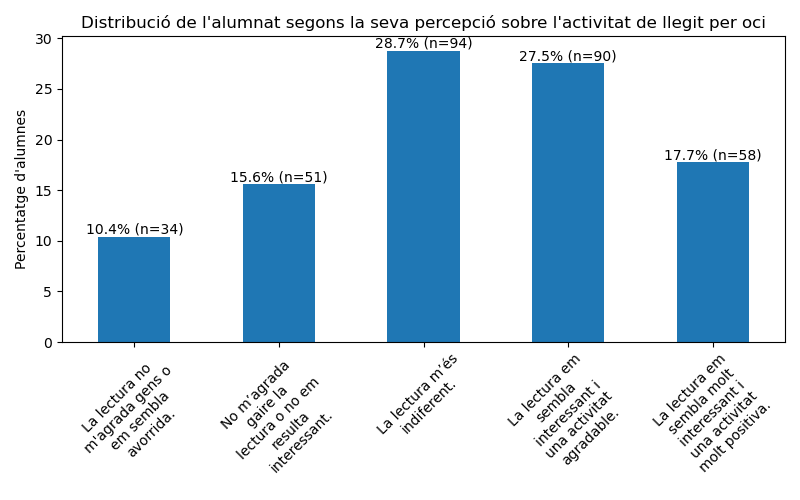
\includegraphics[width=0.85\textwidth]{pictures/9_narrativa_personal.png}
    \caption{Distribució de l'alumnat segons la percepció personal sobre la lectura.}
    \label{fig:narrativa_personal}
\end{figure}

\begin{figure}[H]
    \centering
    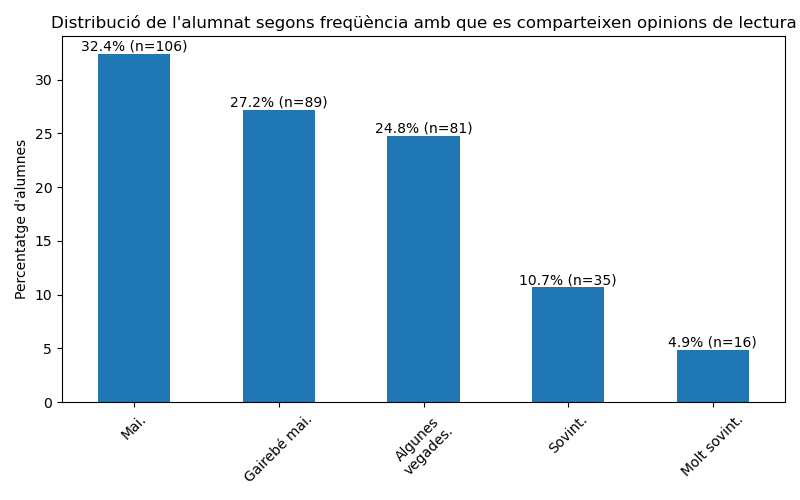
\includegraphics[width=0.85\textwidth]{pictures/9_narrativa_compartir.png}
    \caption{Distribució de l'alumnat segons la freqüència amb què comparteixen opinions sobre lectures.}
    \label{fig:narrativa_compartir}
\end{figure}

\subsection{Gràfics complementaris de lectura per oci i temps dedicat a les noves tecnologies}
\label{graf:tec}

\begin{figure}[H]
    \centering
    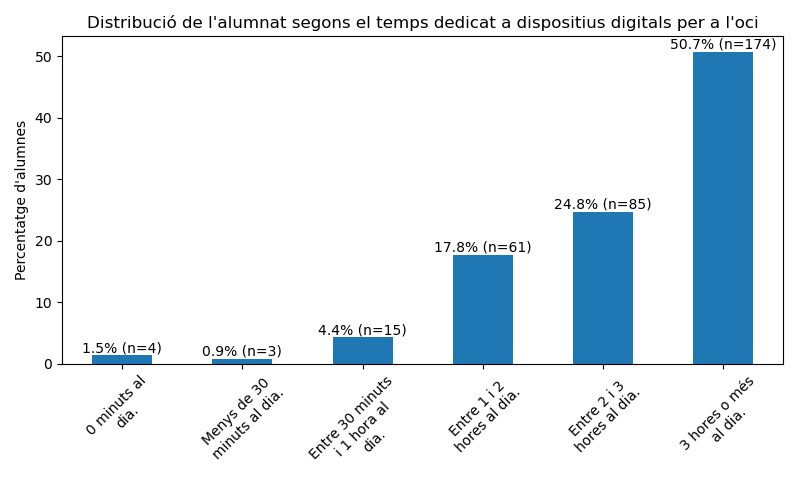
\includegraphics[width=0.85\textwidth]{pictures/10_tec_time.png}
    \caption{Distribució de l'alumnat segons el temps diari dedicat a l'ús de dispositius digitals per a l'oci.}
    \label{fig:tec_time}
\end{figure}

\begin{figure}[H]
    \centering
    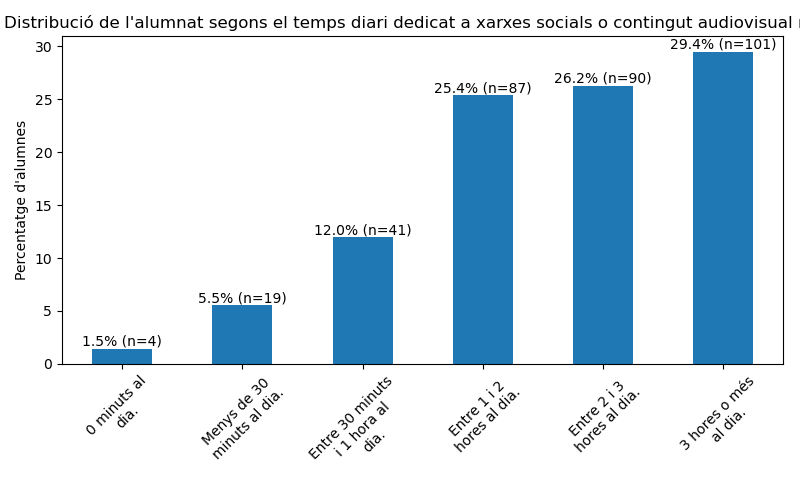
\includegraphics[width=0.85\textwidth]{pictures/10_tric_time.png}
    \caption{Distribució de l'alumnat segons el temps diari dedicat a l'ús de xarxes socials o plataformes de contingut audiovisual ràpid.}
    \label{fig:tric_time}
\end{figure}

\begin{figure}[H]
    \centering
    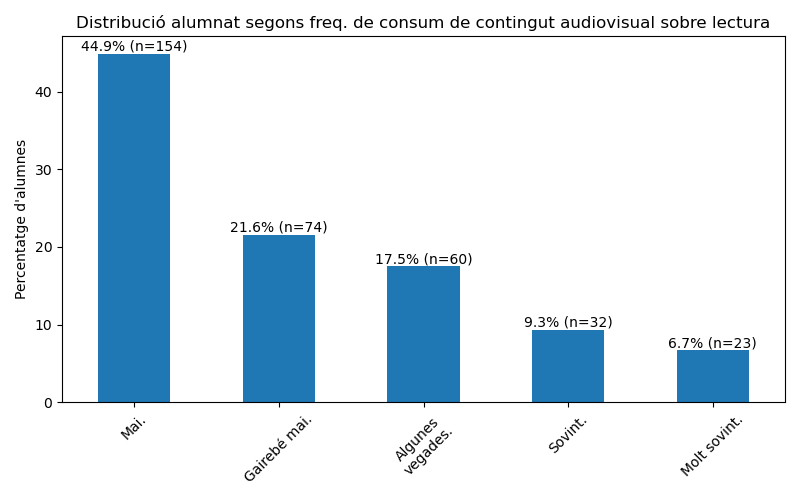
\includegraphics[width=0.85\textwidth]{pictures/10_tric_lite.png}
    \caption{Distribució de l'alumnat segons la freqüència amb què consumeixen contingut audiovisual relacionat amb la lectura.}
    \label{fig:tric_lite}
\end{figure}

\section{Entrevista Semiestructurada Docents}
% =======================================================================
\begin{enumerate}
    \item[] \hspace{-\leftmargin}\textbf{Bloc 0: Experiència docent}
    \item Quines matèries imparteixes actualment?
    \item Llegeixes per oci habitualment? [Llegeix per oci xxxx?]
    \item [] \hspace{-\leftmargin}\textbf{Bloc 1: Hàbits de lectura per oci de l’alumnat}
    \item Creus que els alumnes del centre llegeixen habitualment per oci? Com creus que són els seus hàbits lectors?
    \item Que creus que influeix més en els hàbits lectors dels alumnes del centre?
    \item Quina és la teva percepció sobre la tendència dels hàbits lectors?
    \item Quins factors consideres que estan afavorint més aquesta tendència?
    \item [] \hspace{-\leftmargin}\textbf{Bloc 2: Hàbits de lectura obligatòria de l’alumnat}
    \item En quin grau perceps que es llegeixen les lectures obligatòries de l’escola? Quins factors consideres que afavoreixen aquest fet?
    \item Quina incidència creus que té l’ús de resums d’internet o IA generativa en la realització de treballs o exàmens associats a les lectures obligatòries?
    \item En quin grau perceps que les lectures obligatòries de l’escola són interessants pels alumnes? Creus que s’adapten als seus gustos?
    \item [] \hspace{-\leftmargin}\textbf{Bloc 3: Percepció de la narrativa social de l’alumnat sobre la lectura}
    \item Quina percepció creus que tenen els alumnes sobre la lectura? Per què?
    \item Quins estereotips i prejudicis creus que tenen els adolescents sobre la lectura? Per què?
    \item Creus que els alumnes parlen o comparteixen sovint opinions sobre lectura entre ells?
    \item Quina influència creus que tenen les narratives, els discursos, els estereotips i els prejudicis en els hàbits de lectura dels alumnes?
    \item [] \hspace{-\leftmargin}\textbf{Bloc 4: Influència de les TRIC en els hàbits de lectura de l’alumnat}
    \item Quines oportunitats i quins riscos consideres que aporten les noves tecnologies als hàbits de lectura?
    \item Creus que l’ús de xarxes socials, plataformes de vídeos curts i plataformes de contingut audiovisual competeixen amb el temps que dediquen els alumnes a llegir?
    \item [] \hspace{-\leftmargin}\textbf{Bloc 5: Entorn familiar pro-lector}
    \item Quina influència creus que té un entorn familiar en els hàbits de lectura dels alumnes?
    \item Quan habitualment creus que les famílies durant la infància i l’adolescència dels alumnes creen un entorn que afavoreix els hàbits de lectura?
    \item [] \hspace{-\leftmargin}\textbf{Bloc 6: Hàbits de lectura de l’alumnat i centre}
    \item Com creus que, a nivell de centre, dintre dels marges del sistema educatiu, es podria treballar per afavorir els hàbits de lectura durant la infància i l’adolescència?
\end{enumerate}

Moltes gràcies per participar.

\section{Entrevista Semiestructurada Alumnes}

\begin{enumerate}
    \item [] \hspace{-\leftmargin}\textbf{Bloc 0: Introducció}
    \item Quin curs estàs estudiant actualment?
    \item [] \hspace{-\leftmargin}\textbf{Bloc 1: Hàbits de lectura per oci de l’alumnat}
    \item T’agrada llegir?
    \item Llegeixes habitualment per oci?
    \item Quant llegeixes habitualment?
    \item Què t’agrada llegir?
    \item [] \hspace{-\leftmargin}\textbf{Bloc 2: Hàbits de lectura obligatòria de l’alumnat}
    \item T’agraden les lectures obligatòries de l’escola? Per què?
    \item Creus que, en general, agraden les lectures obligatòries de l’escola als alumnes?
    \item Com acostumes a preparar les lectures obligatòries (llegir-les, resums, vídeos, IA…)?
    \item Han influït les eines d’IA generativa en com et prepares els exàmens o treballs relacionats amb les lectures obligatòries?
    \item [] \hspace{-\leftmargin}\textbf{Bloc 3: Percepció de la narrativa social de l’alumnat sobre la lectura}
    \item Quina percepció creus que tenen els nois i noies de la teva edat sobre la lectura? Per què?
    \item Creus que la percepció, els estereotips i els prejudicis al voltant de la lectura en nois i noies de la teva edat afecten al temps que dediques habitualment a llegir?
    \item Comparteixes opinions sobre lectura amb els teus amics i amigues? Creus que això afecta al temps que dediques habitualment a llegir?
    \item [] \hspace{-\leftmargin}\textbf{Bloc 4: Influència de les TRIC en els hàbits de lectura de l’alumnat}
    \item Creus que les noves tecnologies influeixen positivament o negativament en el temps que dediques habitualment a la lectura per oci?
    \item Quantes hores aproximadament passes al dia en xarxes socials o plataformes com YouTube, TikTok, Netflix, Twitch o similars?
    \item Creus que aquestes plataformes influeixen en el temps que dediques a llegir?
    \item[] \hspace{-\leftmargin}\textbf{Bloc 5: Hàbits de lectura de l’alumnat i sistema educatiu}
    \item Com creus que es podria fomentar la lectura des de l’escola?
\end{enumerate}

Moltes gràcies per participar.

\section{Qüestionari}

\subsectiononumber{Bloc 0: Dades Generals}
Aquest bloc recull dades generals sobre el perfil de l'alumnat.

\begin{enumerate}
    \item \textbf{Curs}
    \begin{itemize}
        \item[$\square$] 3r d'ESO.
        \item[$\square$] 4t d'ESO.
        \item[$\square$] 1r de Batxillerat.
        \item[$\square$] 2n de Batxillerat.
    \end{itemize}

    \item \textbf{Gènere}
    \begin{itemize}
        \item[$\square$] Masculí.
        \item[$\square$] Femení.
        \item[$\square$] Prefereixo no respondre.
    \end{itemize}

    \item \textbf{Itinerari (només si estàs cursant Batxillerat)}
    \begin{itemize}
        \item[$\square$] Ciències i Tecnologia.
        \item[$\square$] Ciències Socials.
    \end{itemize}
\end{enumerate}

% --- BLOC 1 ---
\subsectiononumber{Bloc 1: Hàbits i percepcions de lectura per oci}
Aquest bloc recull dades sobre els hàbits i les percepcions de lectura per oci.

\begin{enumerate}
    \item \textbf{Quant temps a la setmana dediques, de mitjana, a la lectura de llibres o còmics per oci? (Ja sigui en format físic o digital).}
    \begin{itemize}
        \item[$\square$] 0 minuts.
        \item[$\square$] Menys de 30 minuts a la setmana.
        \item[$\square$] Entre 30 minuts i 1 hora a la setmana.
        \item[$\square$] Entre 1 i 2 hores a la setmana.
        \item[$\square$] Entre 2 i 3 hores a la setmana.
        \item[$\square$] 3 hores o més a la setmana.
    \end{itemize}

    \item \textbf{Quants llibres o còmics t'has llegit aproximadament en els últims 12 mesos per oci? (Ja sigui en format físic o digital). Alerta!: Els llibres de lectura obligatòria de l'escola no compten.}
    \begin{itemize}
        \item[$\square$] 0 llibres o còmics.
        \item[$\square$] 1-2 llibres o còmics.
        \item[$\square$] 3-5 llibres o còmics.
        \item[$\square$] 6-10 llibres o còmics.
        \item[$\square$] 11-15 llibres o còmics.
        \item[$\square$] Més de 15 llibres o còmics.
    \end{itemize}

    \item \textbf{En cas que la resposta hagi estat diferent de 0 llibres o còmics, quantes pàgines, de mitjana, tenien aproximadament aquests llibres o còmics?}
    \begin{itemize}
        \item[$\square$] 1-99 pàgines.
        \item[$\square$] 100-299 pàgines.
        \item[$\square$] 300-599 pàgines.
        \item[$\square$] Més de 600 pàgines.
    \end{itemize}

    \item \textbf{Actualment estàs llegint algun llibre o còmic per oci?}
    \begin{itemize}
        \item[$\square$] No.
        \item[$\square$] Sí.
    \end{itemize}

    \item \textbf{Marca ordenadament els 3 gèneres literaris que més llegeixes per oci. Si no llegeixes per oci, no en marquis cap.}
    \begin{itemize}
        \item[$\_$] Novel·la fantàstica.
        \item[$\_$] Novel·la romàntica.
        \item[$\_$] Novel·la de terror.
        \item[$\_$] Novel·la negra.
        \item[$\_$] Novel·la històrica.
        \item[$\_$] Ciència-ficció.
        \item[$\_$] Còmic.
        \item[$\_$] Clàssics.
        \item[$\_$] Poesia.
        \item[$\_$] Assaig (Filosofia, divulgació científica, etc.).
        \item[$\_$] Teatre.
    \end{itemize}
    
    \item \textbf{Quin format de lectura utilitzes més habitualment per a la lectura de llibres o còmics per oci?}
    \begin{itemize}
        \item[$\square$] Físic / en paper.
        \item[$\square$] Digital (ebook).
        \item[$\square$] Digital (llibre Web o PDF en dispositiu electrònic).
        \item[$\square$] No llegeixo per oci.
        \item[$\square$] Altres.
    \end{itemize}

    \item \textbf{Quants cops aproximadament has visitat una biblioteca per llegir o agafar llibres en préstec en els últims 12 mesos per oci?}
    \begin{itemize}
        \item[$\square$] 0 cops.
        \item[$\square$] 1-2 cops.
        \item[$\square$] 3-5 cops.
        \item[$\square$] 6-10 cops.
        \item[$\square$] Més de 10 cops.
    \end{itemize}

    \item \textbf{Quan llegeixes, com acostumen a ser les teves sessions de lectura?}
    \begin{itemize}
        \item[$\square$] Llegeixo gairebé sempre en estones molt curtes (menys de 15 minuts).
        \item[$\square$] Llegeixo sobretot en estones curtes (15-30 minuts).
        \item[$\square$] Combino estones curtes (15-30 minuts) i mitjanes (30-60 minuts).
        \item[$\square$] Llegeixo habitualment en sessions mitjanes (30-60 minuts) i llargues (més d'1 hora seguida).
        \item[$\square$] Depèn molt del moment (no tinc un patró clar).
        \item[$\square$] No llegeixo per oci.
    \end{itemize}

    \item \textbf{Comparteixes opinions de lectura sobre llibres o còmics que has llegit o estàs llegint amb altres persones? (Amics, família, companys de classe, extraescolars, etc.).}
    \begin{itemize}
        \item[$\square$] Mai.
        \item[$\square$] Gairebé mai.
        \item[$\square$] Algunes vegades.
        \item[$\square$] Sovint.
        \item[$\square$] Molt sovint.
    \end{itemize}

    \item \textbf{Veus o escoltes continguts audiovisuals relacionats amb literatura, llibres o còmics per oci? (Veure live-actions, animes o adaptacions no compta; es refereix a recomanacions, reviews, opinions, etc.).}
    \begin{itemize}
        \item[$\square$] Mai.
        \item[$\square$] Gairebé mai.
        \item[$\square$] Algunes vegades.
        \item[$\square$] Sovint.
        \item[$\square$] Molt sovint.
    \end{itemize}
\end{enumerate}

% --- BLOC 2 ---
\subsectiononumber{Bloc 2: Hàbits i percepcions de la lectura acadèmica obligatòria}
Aquest bloc recull dades sobre els hàbits i les percepcions de lectura obligatòria acadèmica.

\begin{enumerate}
    \item \textbf{T'agraden les lectures obligatòries de l'escola?}
    \begin{itemize}
        \item[$\square$] Gens.
        \item[$\square$] Poc.
        \item[$\square$] Regular.
        \item[$\square$] Bastant.
        \item[$\square$] Molt.
    \end{itemize}

    \item \textbf{Amb quina freqüència utilitzes resums d'internet o eines digitals (com IA generativa) per consultar el contingut de les lectures obligatòries de l'escola? (Sigues sincer, aquí no jutgem ni avaluem!).}
    \begin{itemize}
        \item[$\square$] Mai.
        \item[$\square$] Gairebé mai.
        \item[$\square$] Algunes vegades.
        \item[$\square$] Sovint.
        \item[$\square$] Molt sovint.
    \end{itemize}

    \item \textbf{En quin grau llegeixes les lectures obligatòries de l'escola? (Sigues honest, llegir resums d'internet o d'IA generativa no compta).}
    \begin{itemize}
        \item[$\square$] No en llegeixo cap.
        \item[$\square$] En llegeixo poques o molt poques.
        \item[$\square$] En llegeixo aproximadament la meitat.
        \item[$\square$] Les llegeixo gairebé totes.
        \item[$\square$] Les llegeixo totes.
    \end{itemize}

    \item \textbf{Fins a quin punt estàs d'acord amb la següent afirmació: \textit{«Des que utilitzo eines d'IA generativa (ChatGPT, Gemini, Copilot, Claude, etc.), he reduït la lectura de les lectures obligatòries de l'escola»}.}
    \begin{itemize}
        \item[$\square$] Molt en desacord.
        \item[$\square$] Poc d'acord.
        \item[$\square$] Parcialment d'acord.
        \item[$\square$] Bastant d'acord.
        \item[$\square$] Molt d'acord.
    \end{itemize}

    \item \textbf{Fins a quin punt estàs d'acord amb la següent afirmació: \textit{«Llegiria més lectures obligatòries de l'escola si s'adaptessin més als meus gustos»}.}
    \begin{itemize}
        \item[$\square$] Molt en desacord.
        \item[$\square$] Poc d'acord.
        \item[$\square$] Parcialment d'acord.
        \item[$\square$] Bastant d'acord.
        \item[$\square$] Molt d'acord.
    \end{itemize}
\end{enumerate}

% --- BLOC 3 ---
\subsectiononumber{Bloc 3: Discurs i narrativa social adolescent sobre la lectura}
Aquest bloc recull dades sobre el discurs i la narrativa social adolescent al voltant de la lectura.

\begin{enumerate}
    \item \textbf{Amb quina de les següents afirmacions t'identifiques més? (Sigues sincer, aquí no jutgem!).}
    \begin{itemize}
        \item[$\square$] La lectura no m'agrada gens o em sembla avorrida.
        \item[$\square$] No m'agrada gaire la lectura o no em resulta interessant.
        \item[$\square$] La lectura m'és indiferent.
        \item[$\square$] La lectura em sembla interessant i una activitat agradable.
        \item[$\square$] La lectura em sembla molt interessant i una activitat molt positiva.
    \end{itemize}

    \item \textbf{En general, creus que llegir per oci entre els nois i noies de la teva edat és vist com:}
    \begin{itemize}
        \item[$\square$] Una activitat avorrida o poc interessant.
        \item[$\square$] Una activitat normal, sense cap etiqueta especial.
        \item[$\square$] Una activitat positiva o interessant.
    \end{itemize}

    \item \textbf{Quan veus un noi o noia de la teva edat llegint per oci, la teva primera impressió és:}
    \begin{itemize}
        \item[$\square$] Negativa: l'associo amb estrany/estranya, avorrit/avorrida o poc social.
        \item[$\square$] Neutra.
        \item[$\square$] Positiva: l'associo amb intel·ligent o interessant.
    \end{itemize}

    \item \textbf{Fins a quin punt estàs d'acord amb la següent afirmació: \textit{«Si els meus amics o companys de classe llegissin habitualment i parlessin sovint de llibres o còmics, jo també llegiria més»}.}
    \begin{itemize}
        \item[$\square$] Molt en desacord.
        \item[$\square$] Poc d'acord.
        \item[$\square$] Parcialment d'acord.
        \item[$\square$] Bastant d'acord.
        \item[$\square$] Molt d'acord.
    \end{itemize}
\end{enumerate}

% --- BLOC 4 ---
\subsectiononumber{Bloc 4: Ús de les TRIC (Tecnologies per a les Relacions, la Informació i les Comunicacions)}
Aquest bloc recull dades sobre l'ús de les TRIC.

\begin{enumerate}
    \item \textbf{Quant temps al dia dediques, de mitjana, a l'ús de dispositius digitals per a l'oci? (Mòbil, Ordinador, Tablet, Televisió, Smart-watch, etc.).}
    \begin{itemize}
        \item[$\square$] 0 minuts al dia.
        \item[$\square$] Menys de 30 minuts al dia.
        \item[$\square$] Entre 30 minuts i 1 hora al dia.
        \item[$\square$] Entre 1 i 2 hores al dia.
        \item[$\square$] Entre 2 i 3 hores al dia.
        \item[$\square$] 3 hores o més al dia.
    \end{itemize}

    \item \textbf{Quant temps al dia dediques, de mitjana, a utilitzar xarxes socials o veure contingut audiovisual ràpid? (Instagram, TikTok, WhatsApp, X, Telegram, Facebook, Shorts de YouTube).}
    \begin{itemize}
        \item[$\square$] 0 minuts al dia.
        \item[$\square$] Menys de 30 minuts al dia.
        \item[$\square$] Entre 30 minuts i 1 hora al dia.
        \item[$\square$] Entre 1 i 2 hores al dia.
        \item[$\square$] Entre 2 i 3 hores al dia.
        \item[$\square$] 3 hores o més al dia.
    \end{itemize}

    \item \textbf{Quant temps al dia dediques, de mitjana, a veure o sentir contingut audiovisual en Plataformes com Netflix, YouTube, Twitch, Canals de Televisió, Amazon Prime, Spotify, Movistar +, DAZN? (Ja sigui en format vídeo gravat, vídeo en streaming o pòdcast).}
    \begin{itemize}
        \item[$\square$] 0 minuts al dia.
        \item[$\square$] Menys de 30 minuts al dia.
        \item[$\square$] Entre 30 minuts i 1 hora al dia.
        \item[$\square$] Entre 1 i 2 hores al dia.
        \item[$\square$] Entre 2 i 3 hores al dia.
        \item[$\square$] 3 hores o més al dia.
    \end{itemize}

    \item \textbf{Quant temps al dia dediques, de mitjana, a jugar a videojocs? (Ja sigui en PlayStation, Xbox, PC, mòbil, Nintendo Switch, etc.).}
    \begin{itemize}
        \item[$\square$] 0 minuts al dia.
        \item[$\square$] Menys de 30 minuts al dia.
        \item[$\square$] Entre 30 minuts i 1 hora al dia.
        \item[$\square$] Entre 1 i 2 hores al dia.
        \item[$\square$] Entre 2 i 3 hores al dia.
        \item[$\square$] 3 hores o més al dia.
    \end{itemize}

    \item \textbf{Quan llegeixes, acostumes a fer-ho amb música, vídeos o pòdcasts de fons?}
    \begin{itemize}
        \item[$\square$] Mai.
        \item[$\square$] Gairebé mai.
        \item[$\square$] Algunes vegades.
        \item[$\square$] Sovint.
        \item[$\square$] Molt sovint.
    \end{itemize}

    \item \textbf{Amb quina freqüència consultes xarxes socials habitualment mentre llegeixes?}
    \begin{itemize}
        \item[$\square$] Cada 5 minuts aprox.
        \item[$\square$] Cada 15 minuts aprox.
        \item[$\square$] Cada 30 minuts aprox.
        \item[$\square$] Cada hora aprox.
        \item[$\square$] Cada 2 hores aprox.
        \item[$\square$] No miro mai les xarxes socials mentre llegeixo.
    \end{itemize}

    \item \textbf{Fins a quin punt estàs d'acord amb la següent afirmació: \textit{<<Llegiria més llibres o còmics si dediqués menys temps a les xarxes socials i plataformes de vídeos curts (Instagram, TikTok, WhatsApp, X, Shorts, etc.)>>}.}
    \begin{itemize}
        \item[$\square$] Molt en desacord.
        \item[$\square$] Poc d'acord.
        \item[$\square$] Parcialment d'acord.
        \item[$\square$] Bastant d'acord.
        \item[$\square$] Molt d'acord.
    \end{itemize}

    \item \textbf{Fins a quin punt estàs d'acord amb la següent afirmació: \textit{«Llegiria més llibres o còmics si dediqués menys temps a videojocs i/o plataformes de contingut audiovisual (Netflix, YouTube, Twitch, etc.)»}.}
    \begin{itemize}
        \item[$\square$] Molt en desacord.
        \item[$\square$] Poc d'acord.
        \item[$\square$] Parcialment d'acord.
        \item[$\square$] Bastant d'acord.
        \item[$\square$] Molt d'acord.
    \end{itemize}
\end{enumerate}

% --- BLOC 5 ---
\subsectiononumber{Bloc 5: Altres activitats}
Aquest bloc recull dades sobre el discurs i la narrativa social adolescent al voltant de la lectura en relació amb altres activitats.

\begin{enumerate}
    \item \textbf{Quant temps al dia dediques, de mitjana, a l'estudi i la realització de tasques acadèmiques fora de l'horari escolar? (Exàmens, deures, treballs, etc.).}
    \begin{itemize}
        \item[$\square$] 0 minuts al dia.
        \item[$\square$] Menys de 30 minuts al dia.
        \item[$\square$] Entre 30 minuts i 1 hora al dia.
        \item[$\square$] Entre 1 i 2 hores al dia.
        \item[$\square$] Entre 2 i 3 hores al dia.
        \item[$\square$] 3 hores o més al dia.
    \end{itemize}

    \item \textbf{Quant temps al dia dediques, de mitjana, a realitzar activitats relacionades amb la cultura fora de l'horari escolar? (Música, dansa, teatre, pintura, escriptura, visites a museus, etc.).}
    \begin{itemize}
        \item[$\square$] 0 minuts.
        \item[$\square$] Menys de 30 minuts al dia.
        \item[$\square$] Entre 30 minuts i 1 hora al dia.
        \item[$\square$] Entre 1 i 2 hores al dia.
        \item[$\square$] Entre 2 i 3 hores al dia.
        \item[$\square$] 3 hores o més al dia.
    \end{itemize}

    \item \textbf{Quant temps al dia dediques, de mitjana, a la pràctica d'esport fora de l'horari escolar? (Futbol, bàsquet, atletisme, natació, gym, pàdel, etc.).}
    \begin{itemize}
        \item[$\square$] 0 minuts.
        \item[$\square$] Menys de 30 minuts al dia.
        \item[$\square$] Entre 30 minuts i 1 hora al dia.
        \item[$\square$] Entre 1 i 2 hores al dia.
        \item[$\square$] Entre 2 i 3 hores al dia.
        \item[$\square$] 3 hores o més al dia.
    \end{itemize}

    \item \textbf{Quant temps al dia dediques, de mitjana, a quedar amb amics/amigues o parella sentimental fora de l'horari escolar?}
    \begin{itemize}
        \item[$\square$] 0 minuts al dia.
        \item[$\square$] Menys de 30 minuts al dia.
        \item[$\square$] Entre 30 minuts i 1 hora al dia.
        \item[$\square$] Entre 1 i 2 hores al dia.
        \item[$\square$] Entre 2 i 3 hores al dia.
        \item[$\square$] 3 hores o més al dia.
    \end{itemize}

    \item \textbf{Fins a quin punt estàs d'acord amb la següent afirmació: \textit{«Llegiria més llibres o còmics si tingués menys càrrega acadèmica fora d'horari escolar (exàmens, deures, treballs, etc.)»}.}
    \begin{itemize}
        \item[$\square$] Molt en desacord.
        \item[$\square$] Poc d'acord.
        \item[$\square$] Parcialment d'acord.
        \item[$\square$] Bastant d'acord.
        \item[$\square$] Molt d'acord.
    \end{itemize}
\end{enumerate}

% --- BLOC 6 ---
\subsectiononumber{Bloc 6: Entorn familiar pro-lector}
Aquest bloc recull dades sobre l'entorn familiar pro-lector.

\begin{enumerate}
    \item \textbf{Quin és el nivell d'estudis més alt dels teus pares o tutors legals?}
    \begin{itemize}
        \item[$\square$] Educació Primària.
        \item[$\square$] Educació Secundària.
        \item[$\square$] Batxillerat o Cicles Formatius de Grau Mitjà o Superior.
        \item[$\square$] Estudis Universitaris.
        \item[$\square$] No ho sé / Prefereixo no respondre.
    \end{itemize}

    \item \textbf{Durant la teva infància i adolescència, amb quina freqüència has vist als teus pares o tutors legals llegint llibres o còmics per oci?}
    \begin{itemize}
        \item[$\square$] Mai.
        \item[$\square$] Gairebé mai.
        \item[$\square$] Algunes vegades.
        \item[$\square$] Sovint.
        \item[$\square$] Molt sovint.
    \end{itemize}

    \item \textbf{Durant la teva infància i adolescència, amb quina freqüència has parlat amb els teus pares o tutors legals sobre literatura, llibres o còmics?}
    \begin{itemize}
        \item[$\square$] Mai.
        \item[$\square$] Gairebé mai.
        \item[$\square$] Algunes vegades.
        \item[$\square$] Sovint.
        \item[$\square$] Molt sovint.
    \end{itemize}

    \item \textbf{Durant la teva infància i adolescència, amb quina freqüència heu realitzat sessions de lectura conjunta a casa?}
    \begin{itemize}
        \item[$\square$] Mai.
        \item[$\square$] Gairebé mai.
        \item[$\square$] Algunes vegades.
        \item[$\square$] Sovint.
        \item[$\square$] Molt sovint.
    \end{itemize}

    \item \textbf{Durant la teva infància i adolescència, amb quina freqüència aproximadament has anat a la biblioteca amb els teus pares o tutors legals a llegir o agafar llibres en préstec?}
    \begin{itemize}
        \item[$\square$] Mai.
        \item[$\square$] Gairebé mai.
        \item[$\square$] Algunes vegades.
        \item[$\square$] Sovint.
        \item[$\square$] Molt sovint.
    \end{itemize}

    \item \textbf{Fins a quin punt estàs d'acord amb la següent afirmació: \textit{«A casa meva hi ha normes clares sobre el temps que puc dedicar a les pantalles i dispositius digitals»}.}
    \begin{itemize}
        \item[$\square$] Molt en desacord.
        \item[$\square$] Poc d'acord.
        \item[$\square$] Parcialment d'acord.
        \item[$\square$] Bastant d'acord.
        \item[$\square$] Molt d'acord.
    \end{itemize}

    \item \textbf{Quants llibres aproximadament heu tingut a casa durant la teva infància i adolescència?}
    \begin{itemize}
        \item[$\square$] 0 llibres.
        \item[$\square$] Entre 1 i 10 llibres.
        \item[$\square$] Entre 11 i 25 llibres.
        \item[$\square$] Entre 26 i 100 llibres.
        \item[$\square$] Entre 101 i 200 llibres.
        \item[$\square$] Més de 200 llibres.
    \end{itemize}
\end{enumerate}
\end{document}

% =======================================================================
% / Document
% =======================================================================